% Documentation for University of Washington thesis LaTeX document class
% by Jim Fox
% fox@washington.edu
%
%    Revised for version 2015/03/03 of uwthesis.cls
%
%    Printed in twoside style now that that's allowed
%
\documentclass [11pt, proquest] {uwthesis}[2015/03/03] 
 
%
% ==========   Local defs and mods
%

% The following line would print the thesis in a postscript font 
% \usepackage{natbib}
% \def\bibpreamble{\protect\addcontentsline{toc}{chapter}{Bibliography}}

\setcounter{tocdepth}{1}  % Print the chapter and sections to the toc
\usepackage{listings}
\usepackage{url}
\usepackage{amsmath}
\usepackage{amsfonts}
\usepackage{amssymb}
\usepackage{graphicx}
\usepackage{braket}
\usepackage{algorithmicx}
\usepackage{algpseudocode}
\usepackage{algorithm}
\usepackage{textcomp}
\usepackage{gensymb}
\usepackage[T1]{fontenc}
\usepackage{multirow}
\usepackage{longtable}
\usepackage[caption=false]{subfig}

\newcommand{\overbar}[1]{\mkern 1.5mu\overline{\mkern-1.5mu#1\mkern-1.5mu}\mkern 1.5mu}

\begin{document}

%
% ==========   Preliminary pages
%
\prelimpages
 
%
% ----- copyright and title pages
%
\Title{The Suitability of the \LaTeX\ Text Formatter\\
  for Thesis Preparation by Technical and\\
  Non-technical Degree Candidates}
\Author{Nicholas Kullman}
\Year{2013-2016}
\Program{Quantitative Ecology and Resource Management}

\Chair{Sandor F. Toth}{Title of Chair}{School of Environmental and Forest Sciences}
\Signature{David Butman}
\Signature{W. Art Chaovalitwongse}

\copyrightpage

\titlepage  

%
% ----- abstract
%


\setcounter{page}{-1}
\abstract{%
This sample dissertation is an aid to students who are attempting
to format their theses with \LaTeX, a sophisticated
text formatter widely used by mathematicians and scientists everywhere.
 
\begin{itemize}
\item It describes the use of a specialized
macro package developed specifically for thesis production
at the University.
The macros customize \LaTeX\ for the correct thesis style,
allowing the student to concentrate on the substance of
his or her text.%
\footnote{See Appendix A to obtain the source to this
 thesis and the class file.}
\item It demonstrates the solutions to a variety of
formatting challenges found in thesis production.
\item It serves as a template for a real dissertation.
\end{itemize}
}
 
%
% ----- contents & etc.
%
\tableofcontents
\listoffigures
%\listoftables  % I have no tables
 
%
% ----- glossary 
%
\chapter*{Glossary}      % starred form omits the `chapter x'
\addcontentsline{toc}{chapter}{Glossary}
\thispagestyle{plain}
%
\begin{glossary}
\item[argument] replacement text which customizes a \LaTeX\ macro for
each particular usage.
\item[back-up] a copy of a file to be used when catastrophe strikes
the original.  People who make no back-ups deserve
no sympathy.
\item[control sequence] the normal form of a command to \LaTeX.
\item[delimiter] something, often a character, that indicates
the beginning and ending of an argument.
More generally, a delimiter is a field separator.
\item[document class] a file of macros that tailors \LaTeX\ for
a particular document.  The macros described by this thesis
constitute a document class.
\item[document option] a macro or file of macros
that further modifies \LaTeX\ for
a particular document.  The option {\tt[chapternotes]}
constitutes a document option.
\item[figure] illustrated material, including graphs,
diagrams, drawings and photographs.
\item[font] a character set (the alphabet plus digits
and special symbols) of a particular size and style.  A couple of fonts
used in this thesis are twelve point roman and {\sl twelve point roman
slanted}.
\item[footnote] a note placed at the bottom of a page, end of a chapter,
or end of a thesis that comments on or cites a reference
for a designated part of the text.
\item[formatter] (as opposed to a word-processor) arranges printed
material according to instructions embedded in the text.
A word-processor, on the other hand, is normally controlled
by keyboard strokes that move text about on a display.
\item[\LaTeX] simply the ultimate in computerized typesetting.
\item[macro]  a complex control sequence composed of 
other control sequences.
\item[pica] an archaic unit of length.  One pica is twelve points and
six picas is about an inch.
\item[point] a unit of length.  72.27 points equals one inch.
\item[roman]  a conventional printing typestyle using serifs.
the decorations on the ends of letter strokes.
This thesis is set in roman type.
\item[rule] a straight printed line; e.g., \hrulefill.
\item[serif] the decoration at the ends of letter strokes.
\item[table] information placed in a columnar arrangement.
\item[thesis] either a master's thesis or a doctoral dissertation.
This document also refers to itself as a thesis, although it
really is not one.
 
\end{glossary}
 
%
% ----- acknowledgments
%
\acknowledgments{% \vskip2pc
  % {\narrower\noindent
  The author wishes to express sincere appreciation to
  University of Washington, where he has had the opportunity
  to work with the \TeX\ formatting system,
  and to the author of \TeX, Donald Knuth, {\it il miglior fabbro}.
  % \par}
}

%
% ----- dedication
%
\dedication{\begin{center}to my dear wife, Joanna\end{center}}

%
% end of the preliminary pages

%
% ==========      Text pages
%
\textpages
% ======== Introduction to Deschutes National Forest case study

\section{Introduction}
\label{sec:intro}

% Many problems are multi-objective
Many tasks in resource allocation are multi-objective. The design of aircraft involves balancing cost and efficiency \cite{wang2014multi}. Hospitals seek to manage personnel and equipment in order to maximize patient throughput while minimizing cost and required back-up \cite{hutzschenreuter2009evolutionary}. Food production balances processing time with nutrient retention \cite{sendin2010efficient}. Forest managers aim to provide carbon sequestration and wildlife habitat while also maximizing timber revenues \cite{toth2013ecosel}.

% Objs in these problems may conflict
Given a set of solutions to one of these resource allocation problems, a decision maker chooses one to enact. Often, no one solution simultaneously optimizes all objectives, and the decision maker must therefore choose a solution that represents a preferred compromise among them. In such cases, there is some amount of conflict among the objectives. This is in contrast to compatible or harmonious objective relationships in which the objectives improve simultaneously.

% This is what conflict looks like
In the case of aircraft design, cost and efficiency conflict with one another, since more efficient design details tend to cost more. Similarly, hospitals may increase patient throughput by increasing the number of doctors available, but this decision would increase costs. Food production engineers can maximize nutrient retention by reducing the temperature at which processing occurs, but this would lengthen the time required to reach acceptable microbiological levels. Forest managers can maximize timber revenue by removing large old-growth timber, but this would reduce the available wildlife habitat.

% We need to understand conflict so we can make good decisions
While the preferred solution may vary by decision maker, a rational decision maker will prefer one which is Pareto efficient; that is, a solution in which no objective can be improved without compromising another. Multi-objective optimization affords the knowledge of such solutions and can help guide the decision maker by revealing where objectives can be achieved simultaneously and where they conflict. Having access to the set of Pareto efficient solutions may also help the decision maker locate solutions where compromises in one objective allow outweighing improvements in another. For instance the forest manager may discover that forgoing small amounts of timber revenues allows for the sequestration of significantly more carbon. Or the hospital may be able to increase patient throughput substantially if they hire one additional oncologist.
Regardless of whether a decision maker selects a solution providing such gains, the awareness of these relationships enables more informed decision making.

% How might conflict compare across multi-objective systems?
In addition to studying conflict within a system, we may further study it at the super-system level. Consider the situation in which a decision maker oversees multiple systems, each with its own set of Pareto efficient solutions. This could be the case for a manager overseeing multiple hospitals or multiple food processing facilities. Alternatively, each system may correspond to a different regulatory or environmental scenario, such as a forest manager analyzing resource allocation under various realizations of climate change. In such instances, understanding the differences in the conflict relationships between systems may benefit the decision maker, allowing them to ask questions such as: How does the relationship between carbon sequestration and timber revenues vary under different climate change scenarios? Do all hospitals require the same increase in staffing costs to improve patient throughput?

% We don't know, bc no one has asked this question. We're going to, and here's how. Requires a new metric
To date, the multi-objective optimization literature has not addressed conflict at the super-system level. We do so for the first time here, laying a foundation for quantitative conflict analysis. To perform this investigation, we draw on Pareto set indicators and correlation measures commonly used in the field of evolutionary multi-objective optimization (EMO). In EMO, the Pareto set indicators are generally used to assess the performance of algorithms that approximate the Pareto set \cite{zitzler2003performance}, and the correlation measures are used as an aid to increase the computational tractability of the problems encountered in EMO \cite{brockhoff2006all}.

Here we adapt these measures for real-world application, using them to study conflicting management objectives across systems. To further our insight into the origin of conflict within a system, we also propose a new metric for quantifying the conflict between pairs of objectives. The new pairwise conflict metric developed here improves on other commonly used pairwise conflict metrics such as the Pearson and Spearman coefficients. Unlike any current metric, the one we propose simultaneously captures mutual objective achievement and accurately identifies the absence of conflict between objectives. We demonstrate the novel utility of the existing and proposed conflict metrics on a multi-objective scenario-based case study in the Deschutes National Forest.

% Ask the new conflict questions RE system-level conflict and demonstrate how 
In the upcoming sections, we define terminology and the measures of conflict. Then we describe the case study and present its results, including the application of the new and existing conflict metrics. We conclude with discussion, summary, and suggestions for future research.
\section{Methods}
\label{sec:methods}
To analyze conflict across systems and demonstrate a novel application of new and existing conflict metrics we perform a case study on the impacts of climate change on forest management in the Deschutes National Forest. Prior to describing the case study, we first define the terminology used here and describe the methods used to measure conflict.

\subsection{Terminology}
\label{subsec:terminology}
  
\paragraph{The multi-objective problem}
Consider the $M$-objective optimization problem
\begin{align}
\text{Maximize}& \notag \\
& \mathbf{f} = [f_1(\mathbf{x}), f_2(\mathbf{x}), \ldots, f_M(\mathbf{x}) ] \label{eqn:generalObj}\\
\text{subject to}& \notag \\
& \mathbf{x} \in X \label{eqn:generalConstraint}
\end{align}
with \textit{objective functions} $f_i(\mathbf{x}), i \in \{1,\ldots,M\}$ and feasible \textit{decision vectors} (or \textit{solutions}) $\mathbf{x} \in \mathbb{R}^n$ where $n$ is the number of decision variables in the optimization problem. A set of equality and inequality constraints determine the \textit{feasible decision space} $X$. Solutions in $X$ are referenced by a superscript: $X = \{\mathbf{x}^1,\mathbf{x}^2,\ldots,\mathbf{x}^{|X|}\}$. Each objective function $f_i : \mathbb{R}^n \mapsto \mathbb{R}$ maps decision vectors to scalars in $\mathbb{R}$. The vector objective function $\mathbf{f} : X \mapsto \mathbb{R}^M$ maps the feasible decision space to the \textit{objective space} $\mathbb{R}^M$. The set of all objective functions is the \textit{objective set} $\mathcal{M} = \{f_1,\ldots,f_M\}$.

\paragraph{Dominance and frontiers}
A solution $\mathbf{x}^1$ is said to \textit{dominate} another solution $\mathbf{x}^2$ ($\mathbf{x}^1 \succ \mathbf{x}^2$) if
\begin{align}
\exists f_i \in \mathcal{M} : f_i(\mathbf{x}^1) > f_i(\mathbf{x}^2) \text{ and } \forall f_i \in \mathcal{M} \; f_i(\mathbf{x}^1) \ge f_i(\mathbf{x}^2)
\end{align}
A solution $\mathbf{x}^1 \in X$ is \textit{non-dominated} if
\begin{align}
\nexists \mathbf{x}^2 \in X : \mathbf{x}^2 \succ \mathbf{x}^1
\end{align}
The set of non-dominated solutions to the multi-objective problem \eqref{eqn:generalObj} and \eqref{eqn:generalConstraint} is referred to as the \textit{Pareto-optimal set} $P = \{\mathbf{x} \in X | \nexists \mathbf{y} \in X : \mathbf{y} \succ \mathbf{x} \}$.

The \textit{Pareto-optimal frontier}, the \textit{efficient frontier} or, simply, the \textit{frontier} $Z$ is the corresponding set of $M$-dimensional \textit{objective vectors} $\mathbf{z} = [f_1(\mathbf{x}),f_2(\mathbf{x}),\ldots,f_M(\mathbf{x})]$. That is,
\begin{align}
Z = \{\mathbf{z} = [f_1(\mathbf{x}),\ldots,f_M(\mathbf{x})] \:|\: \mathbf{x} \in P\}
\end{align}
Objective vectors' components are referred to in subscripts:
\begin{align}
\mathbf{z} = [z_1, z_2, \ldots, z_M]
\end{align}

\paragraph{Ideal and nadir objective vectors}
The \textit{ideal objective vector} is defined as the vector
\begin{align}
\mathbf{z}^{\text{ideal}} = \max_{\mathbf{x} \in X}\{f_i(\mathbf{x})\} \quad \forall i \in \mathcal{M}.
\end{align}
Analogously, define the nadir solution as the vector
\begin{align}
\mathbf{z}^{\text{nadir}} = \min_{\mathbf{x} \in X}\{f_i(\mathbf{x})\} \quad \forall i \in \mathcal{M}.
\end{align}


\paragraph{Sub-dimensions}
Define the \textit{sub-dimensional objective set} $\mathcal{L} \subset \mathcal{M}$ as a subset of the objective functions $f_i \in \mathcal{M}$. Call the cardinality of this set $L$. The \textit{sub-dimensional objective vector} (specifically, the $L$-dimensional objective vector) for the solution $\mathbf{x}^i$ is the vector denoted $\mathbf{z}^i_\mathcal{L}$ whose components are $z^i_\ell = f_\ell(\mathbf{x}^i)$, $\forall \ell \in \mathcal{L}$. That is, they are the components of $\mathbf{z}^i$ that correspond to the objectives in $\mathcal{L}$.

\paragraph{Trade-offs}
The \textit{trade-off} between two objective vectors $\mathbf{z}^1$ and $\mathbf{z}^2$ is the vector of differences in their objective achievements:
\begin{align}
\mathbf{\tau}^{1,2} = [z^2_1 - z^1_1, z^2_2 - z^1_2, \ldots, z^2_M - z^1_M]
\end{align}
Note that $\mathbf{\tau}^{1,2} = - \mathbf{\tau}^{2,1}$.

Given a sub-dimensional objective set $\mathcal{L}$, define the \textit{sub-dimensional trade-off} $\tau^{1,^2}_\mathcal{L}$ as the vector with components $\tau^{1,2}_\ell$, $\forall \ell \in \mathcal{L}$.

\paragraph{Relative objective achievements, relative objective vectors, and relative trade-offs}
For an objective vector $\mathbf{z}$, its \textit{relative achievement in objective }$i$ is
\begin{align}
\overbar{z_i} = \frac{z_i - z^\text{nadir}_i}{z^\text{ideal}_i - z^\text{nadir}_i},
\end{align}
and the corresponding \textit{relative objective vector} is
\begin{align}
\overbar{\mathbf{z}} = [\overbar{z_1},\overbar{z_2},\ldots,\overbar{z_M}].
\end{align}
For two objective vectors $\mathbf{z}^1$ and $\mathbf{z}^2$, the corresponding \textit{relative trade-off} is
\begin{align}
\overbar{\mathbf{\tau}}^{1,2} = \left[\overbar{z^2_1} - \overbar{z^1_1}, \overbar{z^2_2} - \overbar{z^1_2}, \ldots, \overbar{z^2_M} - \overbar{z^1_M}\right]
\end{align}

\paragraph{Conflict, monotonicity, bundles and stacks}
Objectives in an objective set $\mathcal{L}$ \textit{do not conflict} if the objectives improve simultaneously:
$\forall \mathbf{z}^1, \mathbf{z}^2 \in Z, i \in \mathcal{L}$
\begin{align}
(z^1_i \ge z^2_i) \Rightarrow (z^1_j \ge z^2_j) \quad \forall j \in \mathcal{L}, j \neq i \label{eqn:objPairHarmony}
\end{align}
If \eqref{eqn:objPairHarmony} does not hold, then the objectives conflict. Any pair of objectives $i,j \in \mathcal{M}$ such that equation \eqref{eqn:objPairHarmony} holds are said to \textit{increase monotonically}. Conversely, if 
\begin{align}
(z^1_i \ge z^2_i) \Rightarrow (z^1_j \le z^2_j) \quad \forall \mathbf{z}^1, \mathbf{z}^2 \in Z, j \neq i \label{eqn:objPairMonoDec}
\end{align}
holds, then objectives $i$ and $j$ are said to \textit{decrease monotonically}.

When the objectives represent goods or services, a set of objectives that conflict is defined as a \textit{bundle} and a set of objectives that do not conflict is defined as a \textit{stack}.

Equation \eqref{eqn:objPairHarmony} checks for monotonically increasing relationships among objectives. This means of detecting conflict is functionally equivalent to that used by many studies, such as Brockhoff and Zitzler (2009) \cite{brockhoff2009objective} and Purshouse and Fleming (2003) \cite{purshouse2003conflict}.

\subsection{Conflict and other frontier qualities}
\label{sec:waysToMeasureFrontiers}
% given a system, here's what we're going to measure and how we'll measure it.
Qualities of an efficient frontier that may be of interest to a decision maker include the number of solutions and the spacing of the solutions but especially the conflict among the objectives. To measure conflict over the entire objective set $\mathcal{M}$ we use the hypervolume indicator (see equation \eqref{eqn:hypervol}). The hypervolume indicator measures the proportional volume of the objective space bounded by the frontier. A hypervolume indicator value of $I_{H1} < 1$ indicates conflict among the objectives. We developed a custom algorithm to compute the hypervolume indicator, which is described in detail in \S \ref{chap:appAHypervolumeAlgo}. The unary epsilon indicator also provides a measure of conflict over the entire objective set, representing the distance by which the frontier must be translated in order to cover the ideal solution (see equation \eqref{eqn:unaryEpsIndicator}). If the unary epsilon indicator $I_{\epsilon+} > 0$ the objectives in $\mathcal{M}$ conflict. In the case of multiple frontiers, we use the binary epsilon and binary hypervolume indicators to compare them and determine any dominance relationships (see Table \ref{tab:dominanceRelations}). Details on the computation of all of these metrics can be found in \S \ref{chap:appCComparisonMetrics}.

After concluding that conflict exists (equation \eqref{eqn:objPairHarmony}), another metric is needed to determine which objective pairs contribute to the conflict. Here we propose a new conflict metric created specifically for this purpose.

\subsection{A new measure of pairwise conflict}
\label{sec:newConflictMetric}
% This is our cool new way of drilling down into an objective pair to assess conflict
Consider the frontiers in Figure \ref{fig:ConflictVariesExample}. The conflict between maximization objectives $i$ and $j$ is greatest in Frontier C and least in Frontier A.
\begin{figure}[ht]
\centering
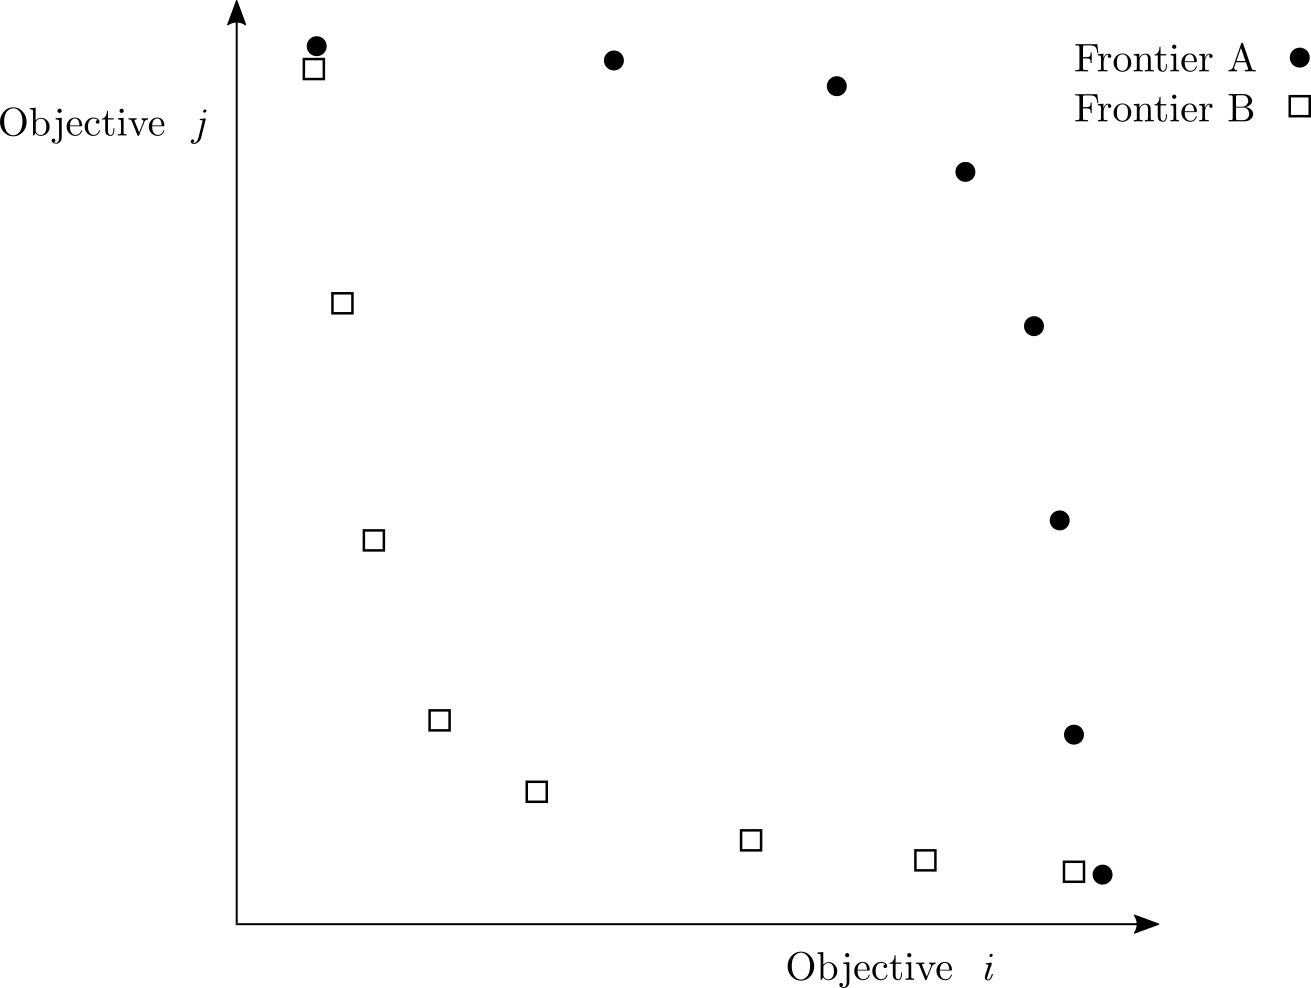
\includegraphics[width=.6\textwidth]{../images/ConflictVariesExample}
\caption[Example of varying conflict between objectives]{Varying conflict between objectives. The conflict between maximization objectives $i$ and $j$ increases from Frontier A to Frontier B to Frontier C.}
\label{fig:ConflictVariesExample}
\end{figure}

Many authors have previously measured conflict between objectives \cite{brockhoff2009objective}\cite{purshouse2003conflict}\cite{gal1977redundant}, with most commonly used metrics deriving from measures of linear correlation (such as the Pearson correlation coefficient \cite{deb2006searching}) or rank correlation (such as Kendall's Tau \cite{kanoulas2009empirical} or Spearman's rho \cite{karande2012application}%, and Zitzler's $\delta$-error \cite{brockhoff2006all}).
). The intended use of these metrics is often the removal of redundant objectives from a many-objective optimization problem. In such cases, measures of monotonicity or correlation alone are adequate. However, the current metrics fall short of providing a quantification of conflict between a pair of objectives. Metrics for linear correlation are limited in their ability to capture the montonicity between objectives, which is the fundamental principle that determines if objectives conflict. Furthermore, both linear and rank correlation metrics fail to capture solutions' objective achievement. Thus, for a more nuanced understanding of the relationship between the objectives, a different metric is required.

Let $\mathbf{z}_{ij}$ be the sub-dimensional objective vector comprised of only the components corresponding to the $i$th and $j$th objectives $\mathbf{z}_{ij} = [z_i,z_j]$. I define the following measure of conflict between objectives $i$ and $j$:
\begin{align}
C_{ij} = \frac{(1-\rho_{ij})\overbar{d}_{ij}}{2 d_{\max,ij}} \label{eqn:defConflict}
\end{align}
where $\overbar{d}_{ij}$ is the average sub-dimensional distance from objective vectors to the ideal solution:
\begin{align}
\overbar{d}_{ij} = \frac{1}{|Z|} \sum_{\mathbf{z} \in Z} ||\mathbf{z}^{\text{ideal}}_{ij} - \mathbf{z}_{ij}||
\end{align}
and
\begin{align}
d_{\max,ij} = ||\mathbf{z}^{\text{ideal}}_{ij} - \mathbf{z}^{\text{nadir}}_{ij}||
\end{align}
and $\rho_{ij}$ is Spearman's rank-correlation coefficient for the solutions' achievements in objectives $i$ and $j$. Note that $C_{ij} \in [0,1)$, taking smaller values when there is less conflict between objectives $i$ and $j$ and larger values when there is more.

The conflict metric proposed here (equation \eqref{eqn:defConflict}) addresses two major issues:
\begin{enumerate}
\item \textbf{Indifference to non-conflicting relationships}. Per equation \eqref{eqn:objPairHarmony}, when an objective $i$ increases monotonically with another objective $j$, the objectives do not conflict. Accordingly, $C_{ij}$ should equal 0 in all such cases. This is true for the new metric, since for monotonically increasing objectives $\rho_{ij} = 1$, so $1-\rho_{ij} = 0$.
\item \textbf{Consideration of objective achievement}. Recall Figure \ref{fig:ConflictVariesExample} and the intuitive notion that the conflict between objectives $i$ and $j$ is stronger in Frontier C than it is in Frontier B than it is in Frontier A. This notion is guided by the idea that the closer objective vectors are to the sub-dimensional ideal solution on average, the less the conflict between the objectives; that is, that greater simultaneous objective provision is indicative of less conflict. The proposed metric accounts for this, while correlation measures do not. In the extreme case of monotonically decreasing objectives, $\frac{(1-\rho_{ij})}{2} = 1$, so $C_{ij} = \frac{\overbar{d}{ij}}{d_{\max,ij}}$. See Figure \ref{fig:WhyOursIsBetter} for an example.
\end{enumerate}
\begin{figure}[ht]
\centering
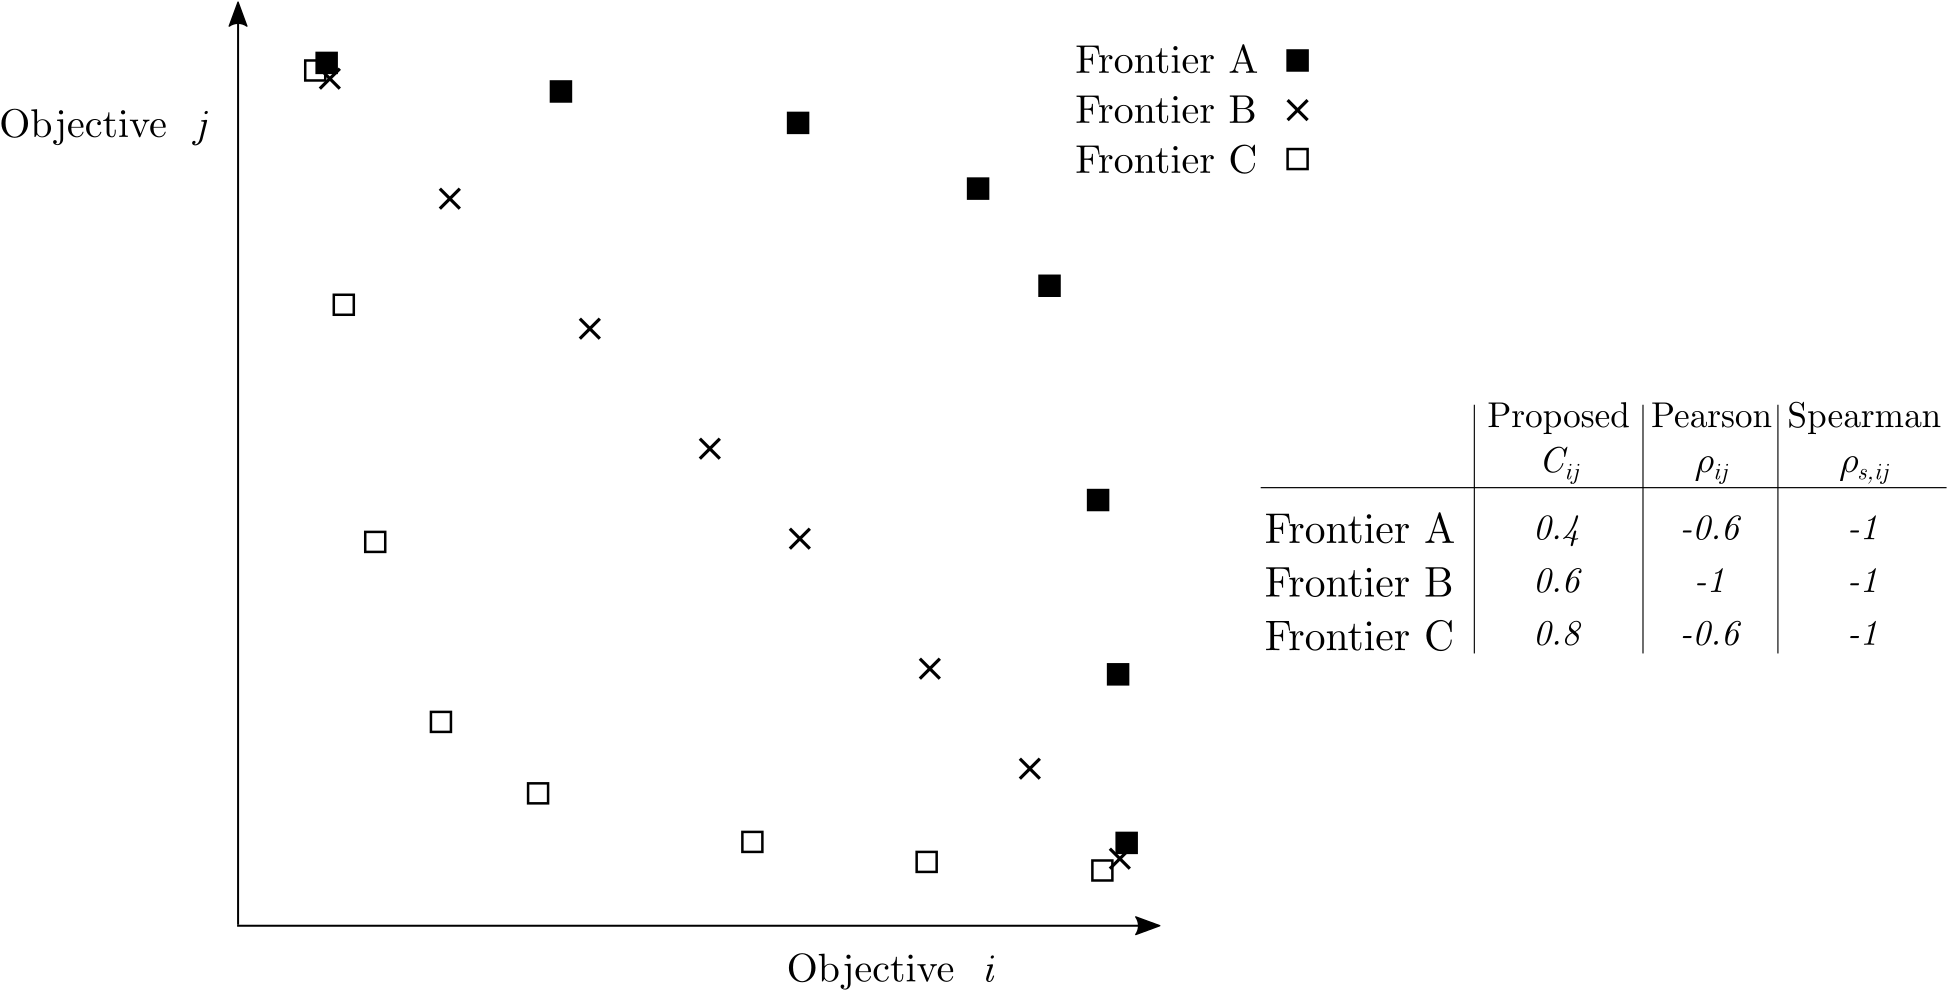
\includegraphics[width=.9\textwidth]{../images/WhyOursIsBetter}
\caption[Comparing the proposed conflict metric to others used in multi-objective optimization]{Comparing the proposed metric for conflict $C_{ij}$ against the Pearson product-moment and the Spearman rank correlation coefficients ($\rho_{ij}$ and $\rho_{s,ij}$, respectively). While the latter two are identical for frontiers A and C, the proposed metric is greater for frontier C than it is for A. This is because it accounts for the average relative distance to the sub-dimensional ideal objective vector.}
\label{fig:WhyOursIsBetter}
\end{figure}

\subsection{Case Study}
\label{sec:caseStudy}
We demonstrate the novel utility of the existing and proposed conflict metrics on a multi-objective scenario-based case study on forest management in the Deschutes National Forest. In the case study, we seek to minimize fire hazard and sediment delivery while maximizing habitat for the northern spotted owl. We compare conflict and objective achievement under multiple climate change scenarios.

\subsubsection{Study system}
\label{subsec:studyArea}
We study the joint provision of forest ecosystem services under multiple climate change scenarios in the Drink Planning Area, located in the Deschutes National Forest. The Drink Area is a 7056 ha area on the east slopes of the Cascade Mountain Range (see Figure \ref{fig:drinkOverview}). Like many forests, the Drink Area is managed for the simultaneous provision of multiple ecosystem services. For this case study, we selected the maximization of habitat for the northern spotted owl, the minimization of fire hazard, and the minimization of sediment delivery. The Forest Service seeks to ensure the sustained provision of these ecosystem services, which may require an understanding of how these ecosystem services are impacted by climate change.

\begin{figure}[ht]
\centering
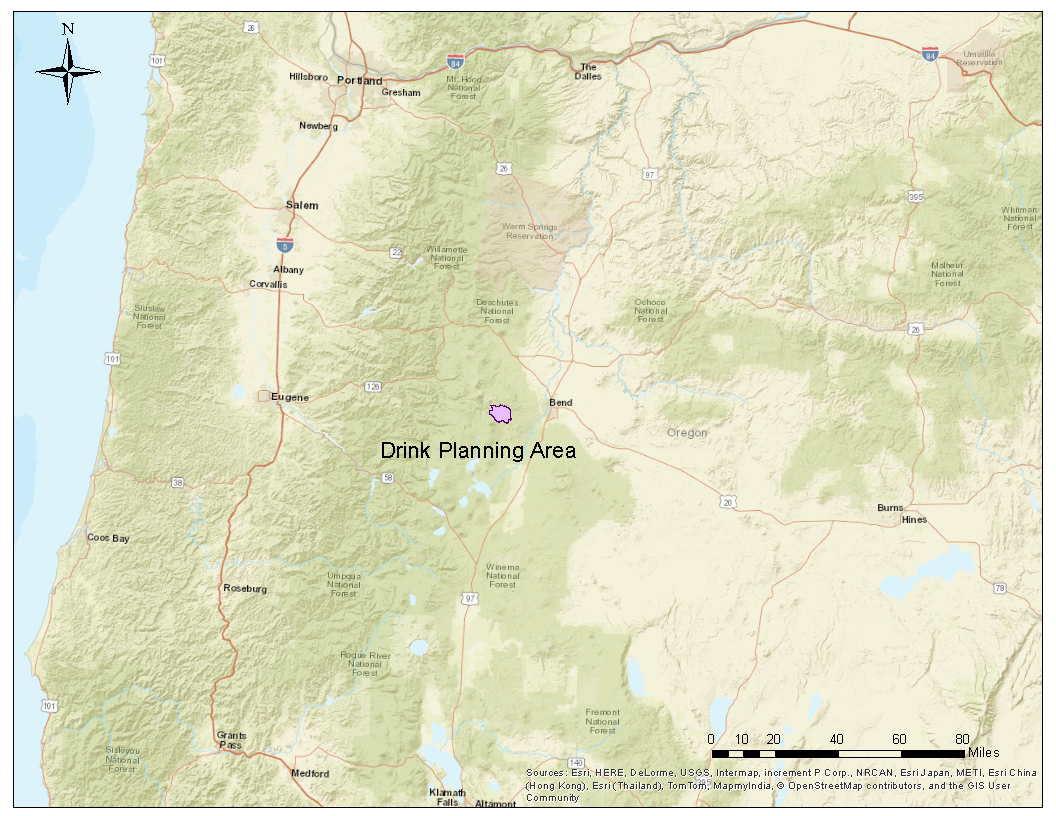
\includegraphics[width=.85\textwidth]{../images/DrinkMap_Overview}
\caption[Overview of the study system, the Drink Planning Area]{Overview of the study system, the Drink Planning Area (in purple), consisting of 7056 ha in the Deschutes National Forest.}
\label{fig:drinkOverview}
\end{figure}

The first ecosystem service is the provision of habitat for the northern spotted owl (NSO) (\textit{Strix occidentalis caurina}). The NSO is a common, if controversial, indicator species in Pacific Northwest forests. Because of the availability of dense old growth forest in the Drink Area, approximately 43\% of the area serves as habitat for the NSO (see Figure \ref{fig:drinkOwlAndWatershed}). The USFS is required to protect this species, because it is listed as threatened and therefore protected by the Endangered Species Act of 1973 \cite{congress1973endangered}.

The second ecosystem service is protection from high severity wildfire. This protection is achieved by applying silvicultural treatments to designated treatment areas (forest stands) throughout the Drink Area. The types of treatments assigned to stands are defined in the appendix, \S \ref{chap:appBTreatmentSpec}. We measure the fire hazard rating of a stand before and after treatment to assess the treatment's efficacy. The fire hazard rating used here is described in more detail later and is summarized in Table \ref{tab:firehazards}. The USFS implements silvicultural treatments to reduce the fire hazard rating in order to protect the habitat of the NSO and also to protect the municipal watershed for the cities of Bend, OR and Sisters, OR which lies largely within the boundaries of the Drink Area (see Figure \ref{fig:drinkOwlAndWatershed}). Wildfires pose a threat to these cities' water supply, because wildfires can cause soil water repellency, surface runoff, and debris torrents \cite{ice2004effects} which would degrade the quality of the watershed. In addition, the Drink Area has never before undergone silvicultural treatments, which increases the expected severity of a fire should one occur. 
\begin{figure}
\centering
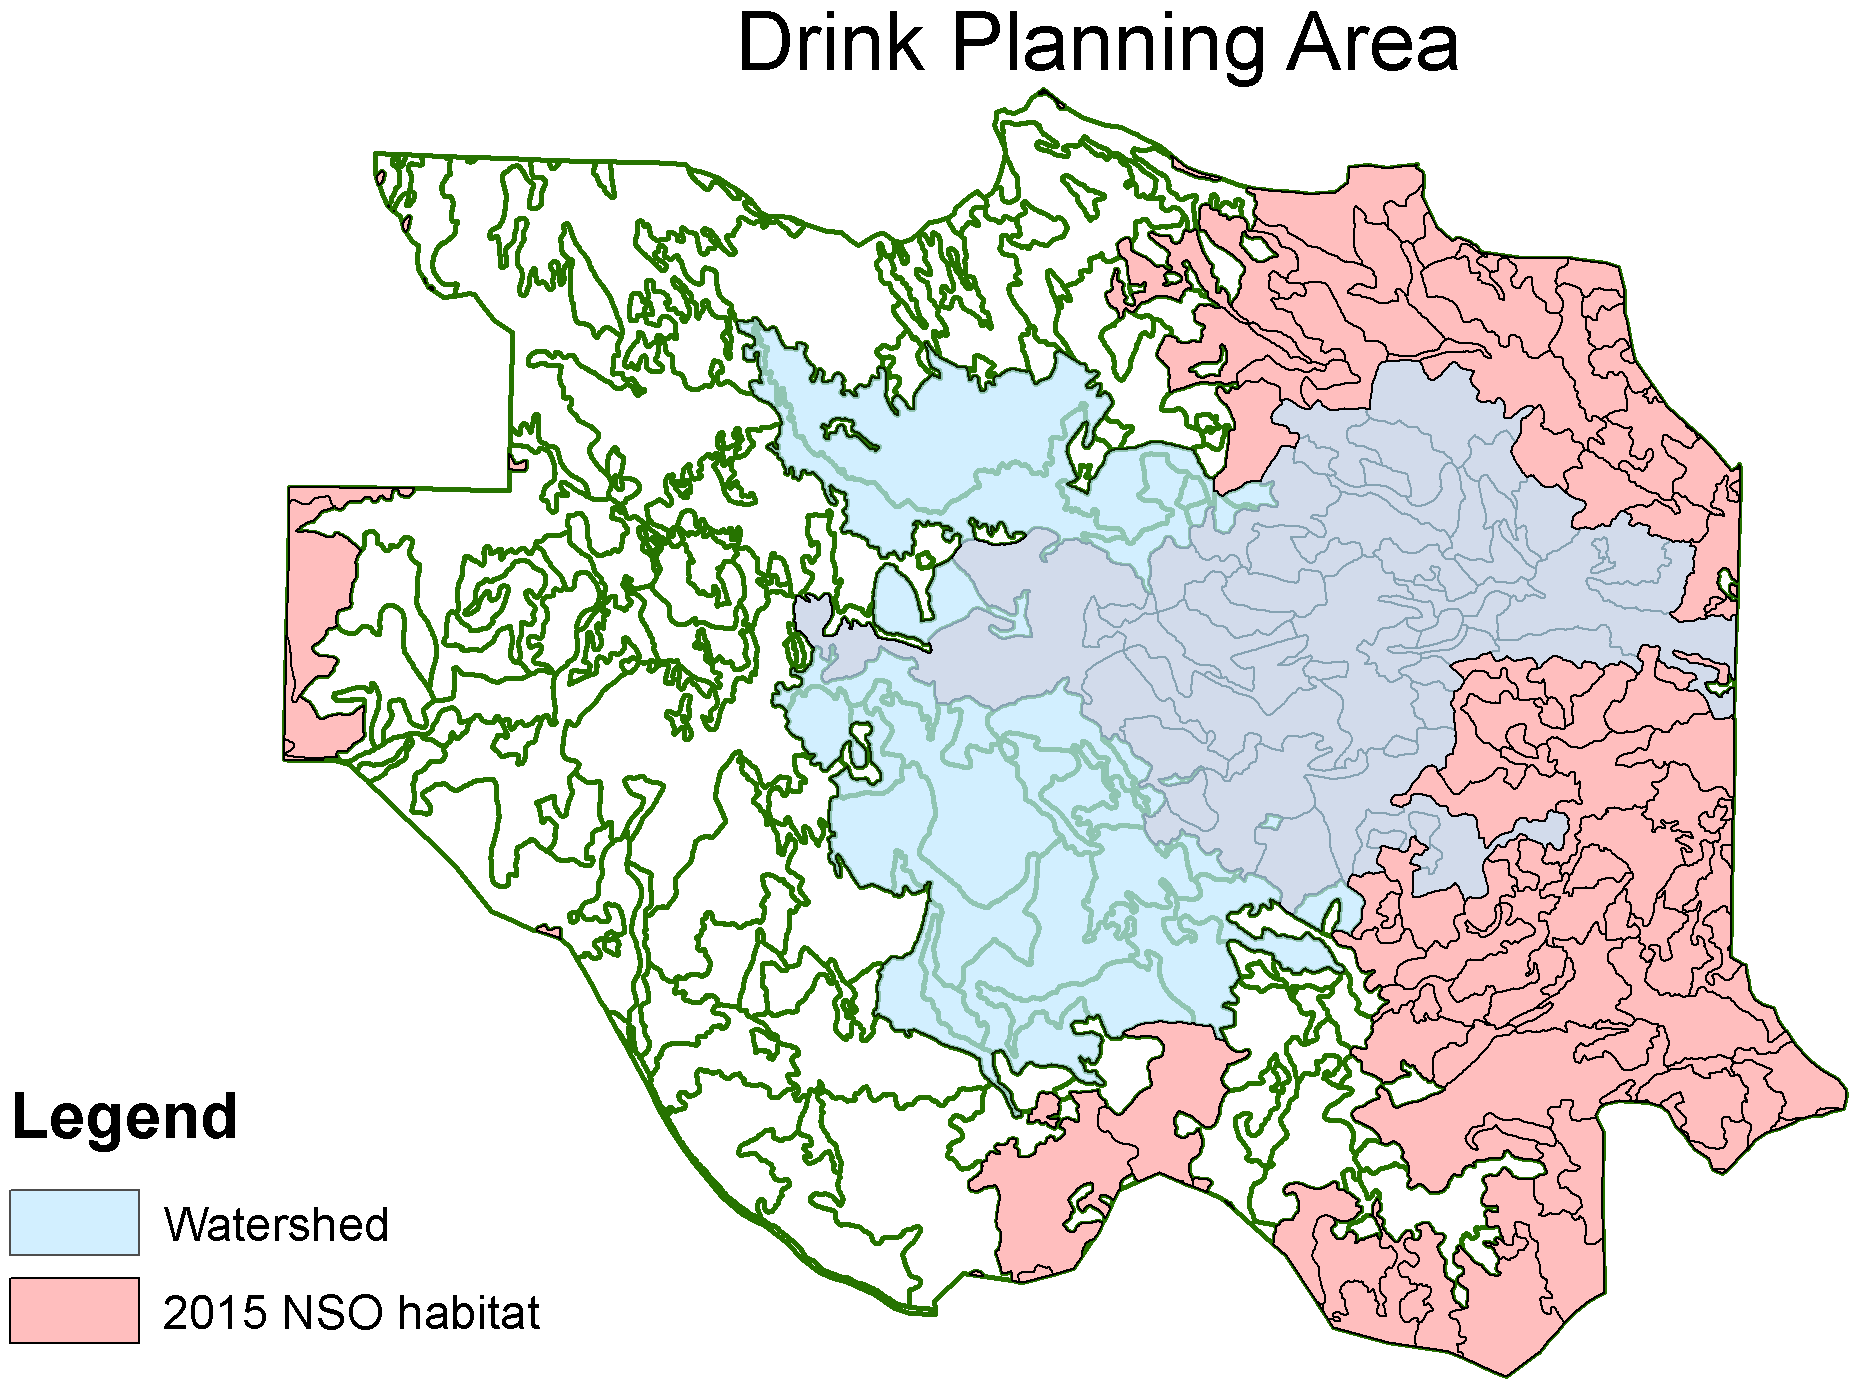
\includegraphics[width=.5\textwidth]{../images/DrinkMap_NSOAndWatershed}
\caption[NSO Habitat and municipal watershed in the Drink Planning Area]{Location of the municipal watershed and the suitable NSO habitat in the Drink area at the beginning of the planning horizon (2015). Interior polygons are the 303 management units.}
\label{fig:drinkOwlAndWatershed}
\end{figure}

Finally, we seek to minimize sediment delivery into the watershed. While the silvicultural treatments intend to provide long-term protection of the watershed, the disturbance caused by implementing the treatments has the potential to induce short-term increases in sediment delivery \cite{o2005conceptual}. This is expected to be especially true in the Drink Area, where local Forest Service staff have noted that the watershed is unusually susceptible to spikes in sediment delivery as a result of foot traffic and other activities that occur within the watershed.

These ecosystem services and their relationships with one another will likely be altered by the changing climate. The extent of these changes will depend on the severity of the realized climate change. Thus, to understand the potential impacts, multiple climate change scenarios representing a range of severities must be considered. The following section describes the climate scenarios considered in this case study.

\subsubsection{Climate Scenarios Considered}
In their assessments on the changing climate, the Intergovernmental Panel on Climate Change (IPCC) uses a scenario-based approach, considering many models of future climates from research groups around the world. They make no attempt to predict which of the future climates is most likely or to quantify the probability of realization of any one scenario. This same scenario-based approach is employed here in studying the potential impacts of climate change on trade-off relationships among bundled ecosystem services. Each scenario considered here results in a distinct multi-objective model and efficient frontier. We choose three climate scenarios for analysis. They were chosen from the set of climate models used by first working group (WG1) in the IPCC's Fifth Assessment (AR5) \cite{ipcc2013climate}. The scenarios will henceforth be referred to as ``None'', ``Ensemble RCP 4.5'' (or ``E45''), and ``Ensemble RCP 8.5'' (or ``E85'').

The first scenario, ``None'', is the assumption of no climate change. While the number of studies incorporating climate change is increasing, this is still the assumption used for many modern studies such as Schroder \textit{et al}. (2013) \cite{schroder2016multi}. Because it has served as the basis for many studies and assumes a static climate resembling today's, the ``None'' climate scenario serves as a control against which to compare the other two climate scenarios.

As their names suggest, the second and third scenarios are ensembles. Each ensemble is an assembly of 17 global circulation models (GCMs) used in IPCC AR5. The selection of component GCMs in the ensembles was performed by the USFS's Climate-Forest Vegetation Simulator (FVS) \cite{dixon2002essential} team. The list of the 17 scenarios included in the ensemble can be found in Crookston (2016) \cite{ClimateModelsInFVSEnsemble}. Each component GCM has a corresponding climate surface which contains a vector of 35 climate parameters at over 11,000 global locations for three time periods (2035, 2065, and 2095). The climate surfaces for the ensembles were created by averaging the values of all component GCMs for each climate parameter and each time period for each location. The result is a climate surface that, while temporally sparse, is spatially robust. Such a configuration is well-suited for use in the Drink Area given the area's variance in elevation and slow vegetation growth.

The two ensembles are comprised of the same 17 GCMs, but the assumed representative concentration pathway (RCP) in the component GCMs differ. The RCP indicates the additional radiative forcing in $W/m^2$ above pre-industrial levels, with higher values of forcing indicative of more severe climate change. The GCMs in the Ensemble RCP 4.5 scenario assume 4.5 $W/m^2$ of additional radiative forcing, and the GCMs in the Ensemble RCP 8.5 scenario assume 8.5 $W/m^2$ of additional radiative forcing.

These three chosen scenarios represent a range of predicted climate change severity, from a $0 \degree C$ warming by the year 2100 under the ``None'' scenario to a $2.6-4.8 \degree C$ warming under RCP 8.5 \cite{ipcc2013climate}. Using a range of climate change severities should produce efficient frontiers and conflict relationships among the objectives that allow for the demonstration of the methods proposed in sections \ref{sec:waysToMeasureFrontiers} and \ref{sec:newConflictMetric}.

\subsection{The Multi-objective Optimization Model}
\label{sec:model}
In order to determine trade-off relationships among ecosystem services under each climate scenario, I employ multi-objective spatial optimization. This section describes the multi-objective zero-one mathematical program to optimize the joint provision of ecosystem services in the Drink Area. The model operates over an 80-year planning horizon (2015-2095) in which it assigns silvicultural treatments to forest stands that will be performed in the first or second 20 year period (2015-2035 or 2035-2055). Determining which treatment type to apply to a stand was done \textit{a priori} and is entirely dependent on silvicultural characteristics; the rules governing this assignment of treatment type can be found in the appendix, \S \ref{chap:appBTreatmentSpec}.

\begin{figure}
\centering
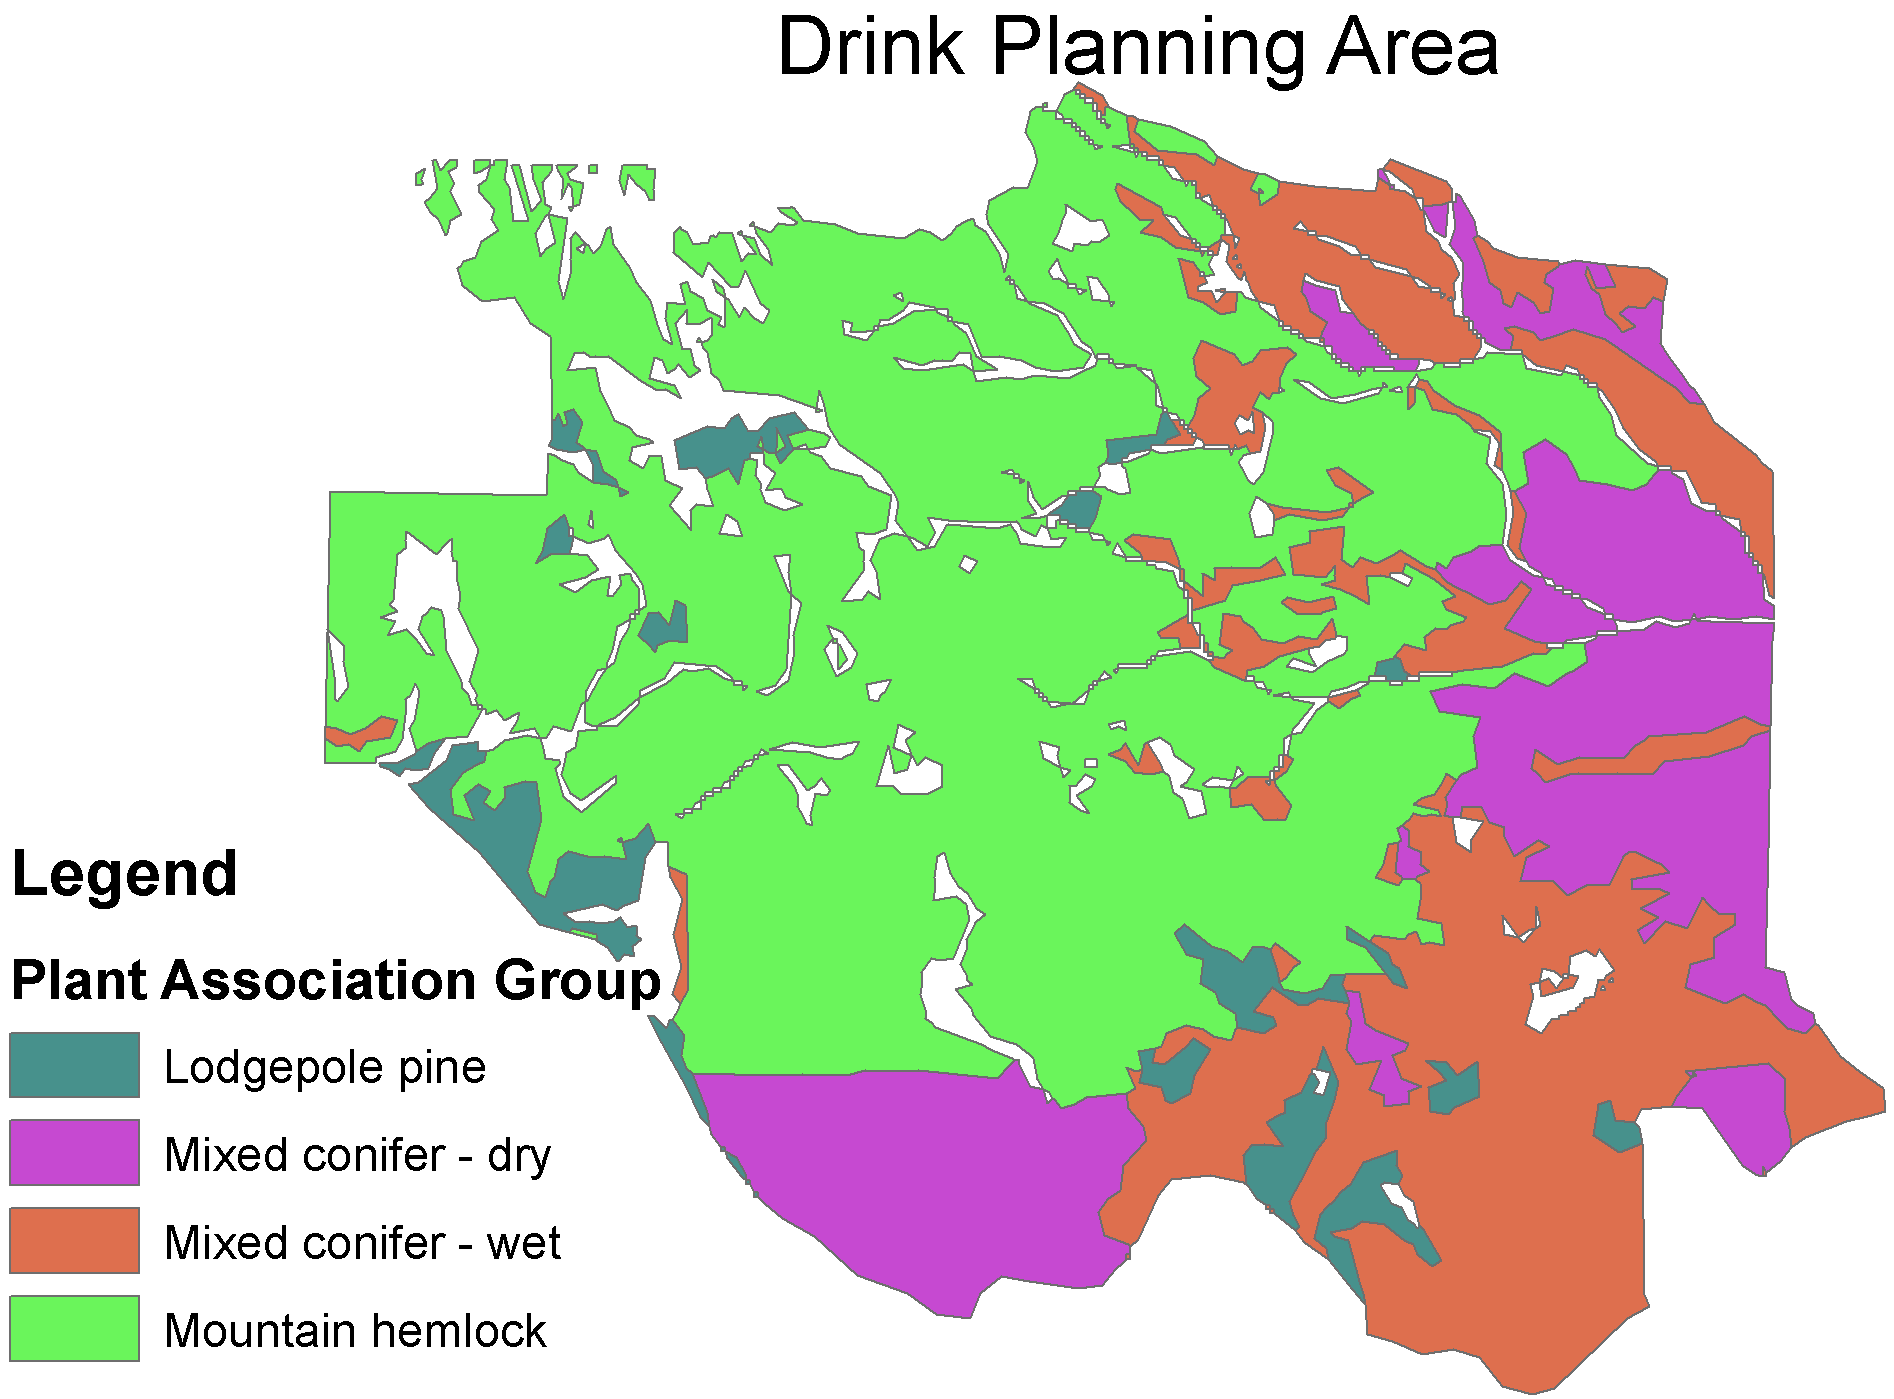
\includegraphics[width=.5\textwidth]{../images/DrinkMap_PAGs}
\caption[Plant association groups in the Drink Planning Area]{Plant association groups in the Drink Planning Area that were selected for potential treatments. Other plant association groups exist in the area but were not considered for treatment.}
\label{fig:drinkPAGs}
\end{figure}

The model minimizes the fire hazard rating of the Drink at the end of the 80-year planning horizon, maximizes the area of NSO habitat at the end of each planning period, and minimizes the short-term spikes in sediment delivery resulting from the application of silvicultural treatments.

Treatments are assumed to be performed at the midpoint year in the treatment period, years 2025 and 2045 for the first and second periods, respectively. A schematic of the planning horizon including the time of these events is shown in Figure \ref{fig:drinkPlanningHorizon}.

\begin{figure}
\centering
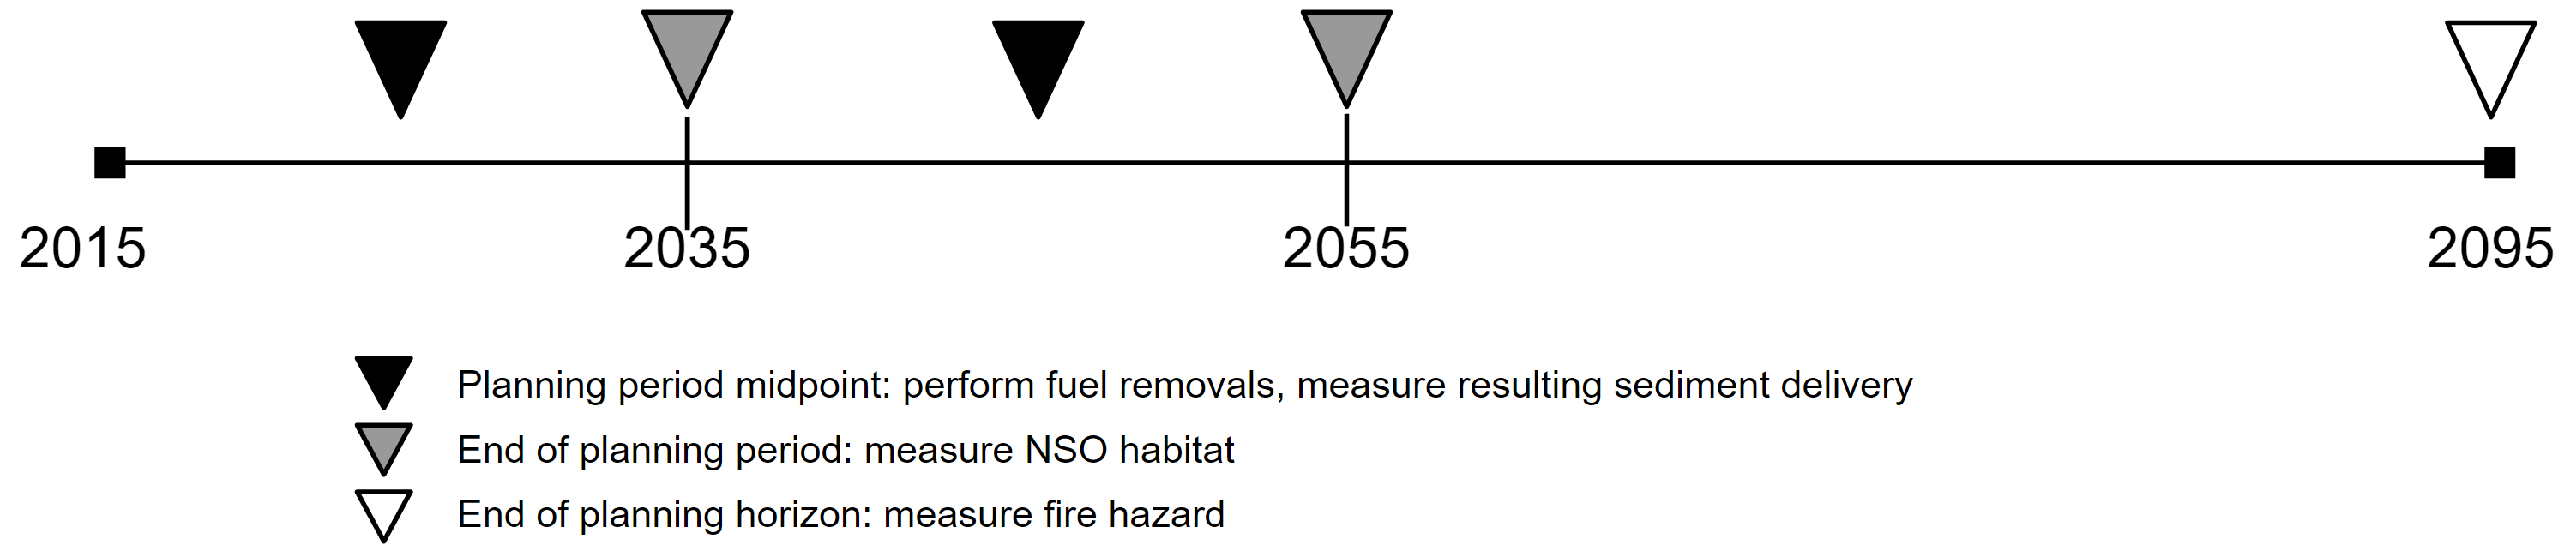
\includegraphics[width=.85\textwidth]{../images/Drink_PlanningHorizon_Sketch}
\caption[Planning horizon schematic]{The planning horizon used in the analysis spans the 80 year period from 2015 to 2095. Treatments may be performed in the first period, the second period, both, or neither. Treatments are assumed to be performed at the mid-point years of each period (black triangles). Sediment delivery is measured on treatment years. Stands' suitability for NSO habitat is measured at the end of the planning periods (gray triangles), and stands' fire hazard ratings are measured at the end of the planning horizon (white triangle).}
\label{fig:drinkPlanningHorizon}
\end{figure}

\subsubsection{Notation}
The following notation is used throughout the model:
\paragraph{Parameters}
\begin{itemize}
\item \textbf{$i \in I$:} the set of all 303 forest stands comprising the Drink area
\item \textbf{$r \in R$:} the set of treatment schedule prescriptions:
	$$
	r =
	\begin{cases}
	1 &\text{ treatment applied in the first period (2015-2035)}\\
	2 &\text{ treatment applied in the second period (2035-2055)}\\
	3 &\text{ treatment applied in both periods}\\
	0 &\text{ no treatment applied in either period}
	\end{cases}
	$$
\item \textbf{$F_{i,r}$:} the area-weighted fire hazard rating of stand $i$ at the end of the planning horizon if prescribed to treatment schedule $r$
\item \textbf{$I_{\omega,t}$:} the set of stands that can qualify as NSO habitat at the end of planning period $t$
\item \textbf{$a_i$:} the area of stand $i$
\item \textbf{$e$:} the discount factor applied to NSO habitat that is less than 200 ha in size
\item \textbf{$j \in R_{i,t}$:} the set of treatment schedules such that stand $i$ qualifies as NSO habitat in planning period $t$
\item \textbf{$s_{i,t}$:} the contribution in tons of sediment delivered from performing fuel treatments on stand $i$ in planning period $t$
\item \textbf{$c \in C$:} the set of all clusters of stands whose combined area exceeds 200 hectares
\item \textbf{$i \in D_c$:} the set of all stands that comprise cluster $c$
\item \textbf{$c \in C_i$:} the set of all clusters that contain stand $i$
\item \textbf{$A$:} the maximum area in hectares that may be treated in either planning period
\item \textbf{$\ell$, $u$:} the lower and upper bounds, respectively, on the relative fluctuation in the area treated in periods 1 and 2
\end{itemize}

\paragraph{Decision Variables}
$$
x_{i,r} = \begin{cases}
1 &\text{ if stand $i$ is prescribed to treatment schedule $r$}\\
0 &\text{ otherwise}
\end{cases}
$$ 

\paragraph{Indicator Variables}
\begin{itemize}
\item \textbf{$q_{c,t} = 1$} if all stands in cluster $c$ qualify as NSO habitat in planning period $t$ and $q_{c,t} = 0$ otherwise
\item \textbf{$p_{i,t} = 1$} if in planning period $t$ stand $i$ is part of a cluster $c$ such that $q_{c,t} = 1$; $p_{i,t} = 0$ otherwise
\end{itemize}

\paragraph{Accounting Variables}
\begin{itemize}
\item \textbf{$S_t$:} the contribution in tons of sediment delivered from performing fuel treatments in planning period $t$
\item \textbf{$O_t$:} the amount of NSO habitat in hectares at the end of planning period $t$
\item \textbf{$H_t$:} the area in hectares treated in planning period $t$
\end{itemize}

\subsubsection{Parameterization}
The model was parameterized as follows:
\begin{itemize}
\item \textbf{$F_{i,r}$:} the metric for fire hazard rating used in this analysis originated in the work by Schroder \textit{et al.} \cite{schroder2016multi}. This metric was developed for the Drink area. It uses fire characteristics from Anderson's fuel models \cite{anderson1982aids} to assign a fire hazard rating. I expanded the rating system to include fuel models not present in Schroder \textit{et al.} See Table \ref{tab:firehazards}.

The stands' fuels and vegetation characteristics to determine the fire hazard rating were generated using the US Forest Service's Climate-Forest Vegetation Simulator (FVS). Input vegetation data to Climate-FVS came from the 2012 GNN structure map (\url{http://lemma.forestry.oregonstate.edu/data/structure-maps}) from Oregon State University's Landscape Ecology, Modeling, Mapping \& Analysis (LEMMA) group. Plots from the LEMMA database were mapped to the stands in the Drink area in order to produce tree and stand lists. These lists were used with Climate-FVS to simulate the stands' vegetation and fuels characteristics forward for the duration of the planning horizon under each climate scenario. Input climate data for Climate-FVS was obtained through the Climate-FVS climate data server \cite{climateFVSReadyData}.
\item \textbf{$I_{\omega,t}$:} the set of stands that qualify as NSO habitat at the end of a planning period $t$ are those that meet the following three criteria, as specified by the USFS:
	\begin{enumerate}
	\item elevation less than 1830 m
	\item the presence of trees with DBH no less than 76 cm
	\item canopy closure of at least 60\%
	\end{enumerate}
The elevation requirement was checked using a digital elevation model from the US Department of Agriculture's GeoSpatial Data Gateway; canopy closure and large tree requirements were determined using the simulated vegetation characteristics output from Climate-FVS.

To account for the NSO's large habitat requirements, stands must also be members of a cluster exceeding 200 ha in size, the entirety of which meets the aforementioned NSO habitat criteria. Stands not part of such a cluster have their contributions to owl habitat discounted by a factor of $e$.
\item \textbf{$e$:} the discount factor for sub-200 ha NSO habitat was set to $e = 0.5$ following the convention used in Schroder \textit{et al.} \cite{schroder2016multi}.
\item \textbf{$j \in R_{i,t}$:} each stand-treatment schedule combination is evaluated at the end of each planning period to determine its suitability as NSO habitat. Treatment schedules for which stand $i$ meets the NSO habitat criteria at the end of treatment period $t$ become members of the set $R_{i,t}$. 
\item \textbf{$s_{i,t}$:} the contributions of sediment delivery from treatment of stand $i$ in period $t$ were determined using the Watershed Erosion Prediction Project (WEPP) online GIS tool \cite{frankenberger2011development}. This tool takes as input soil textures, treatment types, duration of simulation, and custom climate data. Soil texture data for the Drink area was obtained from the USDA's Soil Survey Geographic (SSURGO) database, treatment types are those specified in \S \ref{chap:appBTreatmentSpec}, and the years of simulation correspond to the treatment years in the model's planning horizon (2015-2095). The custom climate data are those described above for use with Climate-FVS, obtained through the Climate-FVS data server.
\item \textbf{$C$,$D_c$,$C_i$:} the formulation of clusters was performed \textit{a priori} according to the algorithm used in Rebain and McDill (2003) \cite{rebain2003mixed}. The enumerated clusters can then be used to immediately determine cluster members $D_c$ and stand-owning clusters $C_i$.
\item \textbf{$A$:} the maximum area that may be treated in either planning period was defined to be 6000 acres, or approximately 2428 ha
\item \textbf{$\ell$, $u$:} the relative fluctuation in the area treated in periods 1 and 2 was defined to be 20\%. That is, the lower bound $\ell = 0.8$, and the upper bound $u = 1.2$.
\end{itemize}
\begin{table}[!ht]
\centering
\resizebox{\textwidth}{!}{%
\begin{tabular}{l|c|crrr}
\multicolumn{1}{c|}{Fuel Model} & \multicolumn{1}{c|}{\textbf{Fire Hazard Rating}} & \multicolumn{1}{c}{Group} & \multicolumn{1}{c}{Flame length (m)} & \multicolumn{1}{c}{Rate of spread (m/hr)} & \multicolumn{1}{c}{Total fuel load (tons/ha)} \\ \hline
4*                              & \textbf{5}                                       & Shrub                     & 5.79                                 & 1508.76                                   & 32.12                                         \\
5                               & \textbf{4}                                       & Shrub                     & 1.22                                 & 362.10                                    & 8.65                                          \\
8                               & \textbf{1}                                       & Timber                    & 0.30                                 & 32.19                                     & 12.36                                         \\
9*                              & \textbf{2}                                       & Timber                    & 0.79                                 & 150.88                                    & 8.65                                          \\
10                              & \textbf{2}                                       & Timber                    & 1.46                                 & 158.92                                    & 29.65                                         \\
11*                             & \textbf{2}                                       & Logging Slash             & 1.07                                 & 120.7                                     & 28.42                                         \\
12                              & \textbf{4}                                       & Logging Slash             & 2.44                                 & 261.52                                    & 85.50                                         \\
13                              & \textbf{5}                                       & Logging Slash             & 3.20                                 & 271.58                                    & 143.57                                       
\end{tabular}%
}
\caption[Fire hazard ratings used in multi-objective model]{Fire hazard rating system used here, originally employed by Schroder \textit{et al.} \cite{schroder2016multi}.\\
Asterisks (*) denote fuel models not present in Schroder \textit{et al.}\\
The fuel model column refers to the Anderson fuel model ratings \cite{anderson1982aids}.}
\label{tab:firehazards}
\end{table}

\subsubsection{Formulation}
The formulation of the model is as follows:
\begin{align}
Minimize \quad & \notag\\
&\sum_{i\in I}\sum_{r\in R} F_{i,r} x_{i,r} \label{eqn:objFire} \\
&\max \{S_1,S_2\} \label{eqn:objSediment} \\
Maximize \quad & \notag\\
&\min \{O_1,O_2\} \label{eqn:objOwl}
\end{align}
Subject to:
\begin{align}
\sum_{i\in I_{\omega,t}} \left(a_i p_{i,t} + e a_i \left( \sum_{j \in R_{i,t}} x_{i,j}-p_{i,t} \right) \right) &= O_t \qquad \forall t \in \{1,2\} \label{eqn:constraintDefOwl}\\
\sum_{i\in I} \sum_{r\in 1,3} s_{i,1} x_{i,r} &= S_1 \label{eqn:constraintSediment1} \\
\sum_{i\in I} \sum_{r\in 2,3} s_{i,2} x_{i,r} &= S_2 \label{eqn:constraintSediment2} \\
\sum_{i \in D_c} \sum_{j \in R_{i,t}} x_{i,j} - |c| q_{c,t} &\ge 0 \qquad \forall t \in \{1,2\}, c \in C \label{eqn:constraintClusterTriggers} \\
\sum_{c \in C_i} q_{c,t} - p_{i,t} &\ge 0 \qquad \forall t \in \{1,2\}, i \in I_{\omega,t} \label{eqn:constraintPVarTriggers} \\
\sum_{r \in R} x_{i,r} &= 1  \qquad \forall i \in I \label{eqn:constraintOnePrescrip} \\
\sum_{i \in I} \sum_{r \in 1,3} a_i x_{i,r} &= H_1 \label{eqn:constraintAreaAcctg1} \\
\sum_{i \in I} \sum_{r \in 2,3} a_i x_{i,r} &= H_2 \label{eqn:constraintAreaAcctg2} \\
H_t &\le A \qquad \forall t \in \{1,2\} \label{eqn:constraintAreaRestr} \\
\ell H_1 - H_2 &\le 0 \label{eqn:constraintAreaFlucL} \\
-u H_1 + H_2 &\le 0 \label{eqn:constraintAreaFlucU} \\
x_{i,r}, p_i, q_c \in \{0,1\} \quad &\forall i \in I, r \in R, c \in C \label{eqn:constraintNonNeg}
\end{align}

Equations \eqref{eqn:objFire}-\eqref{eqn:objOwl} are the objective functions: equation \eqref{eqn:objFire} minimizes the cumulative fire hazard rating of the Drink area at the end of the 80-year planning horizon, equation \eqref{eqn:objSediment} minimizes the maximum peak in sediment delivery for the two planning periods, and equation \eqref{eqn:objOwl} maximizes the minimum NSO habitat available at the end of the planning periods. Equation set \eqref{eqn:constraintDefOwl} defines the amount of NSO habitat available at the end of the planning horizons. Note that if stand $i$ does not belong to a cluster of NSO habitat exceeding 200 hectares, then its area contribution to total NSO habitat is discounted by a factor of $e$. Equations \eqref{eqn:constraintSediment1} and \eqref{eqn:constraintSediment2} define the sediment delivered in planning periods one and two, respectively.

Inequality set \eqref{eqn:constraintClusterTriggers} controls the value of the cluster variables $q_{c,t}$ indicating clusters meeting NSO habitat criteria in each of the planning periods. Inequality set \eqref{eqn:constraintPVarTriggers} controls the value of the $p_{i,t}$ variables indicating stands' inclusion in NSO habitat clusters.

The set of equalities \eqref{eqn:constraintOnePrescrip} enforces the logical constraint that each stand must be prescribed to exactly one treatment schedule. Equations \eqref{eqn:constraintAreaAcctg1} and \eqref{eqn:constraintAreaAcctg2} are accounting constraints for the total area treated in each planning period, and inequalities \eqref{eqn:constraintAreaRestr} ensure that this area does not exceed the predefined per-period maximum. Inequalities \eqref{eqn:constraintAreaFlucL} and \eqref{eqn:constraintAreaFlucU} bound the fluctuation in treated area between the planning periods. Finally, constraint \eqref{eqn:constraintNonNeg} defines the decision and indicator variables as binary.

\subsection{Model Solution and Comparing Efficient Frontiers}
I developed an implementation of T\'{o}th's Alpha-Delta algorithm \cite{TothThesis} to solve the models utilizing the IBM ILOG CPLEX optimization engine. For a problem with $N$ objectives, the Alpha-Delta algorithm finds the optimal set of solutions by iteratively slicing the $N$-dimensional objective space with a tilted $N-1$ dimensional plane. The algorithm was implemented using an alpha parameter of $\alpha = .01$ and delta parameters of $\delta_{Hab} = 1$ ha and $\delta_{Sed} = 2$ tons for the NSO habitat and sediment delivery objectives, respectively.

The solution to a bounded and non-degenerate multi-objective optimization problem with $N$ objectives is a set of objective vectors (also called ``solutions'') $\mathbf{z} \in Z$ where $\mathbf{z}=[z^1,\ldots,z^N]$. The set of solutions $Z$ is referred to as the Pareto-optimal frontier or efficient frontier or, simply, frontier. The solutions comprising an efficient frontier have the special relationship such that no component of a solution $\mathbf{z}^i$ can be improved upon without one of the other components $\mathbf{z}^j$ ($j \neq i$) degrading. This quality is known as Pareto efficiency. For example, this relationship in the current problem means that further reducing the value of fire hazard in a solution would result in either additional sediment delivery, a reduction of NSO habitat, or both.

Thus the efficient frontier provides information on the trade-off relationship that exists between ecosystem services. Parameterizing and solving the above model for each of the climate scenarios generates three frontiers: $Z_{\text{None}}$, $Z_{4.5}$, and $Z_{8.5}$ for the None, Ensemble RCP 4.5, and Ensemble RCP 8.5 scenarios, respectively. Since climate data alone differentiates the models and their resulting frontiers, comparing the frontiers reveals the impacts of climate on the trade-off relationships among the ecosystem services. However, no standardized procedure exists to compare frontiers.

One applicable metric to compare frontiers is the volume of the $N$-dimensional objective space bounded by the frontier, known as the hypervolume indicator. Together with S\'{a}ndor T\'{o}th, I devised an algorithm to compute the value of the hypervolume indicator any general $N$-dimensional frontier. The algorithm proceeds by sorting the solutions according to one objective, then iteratively adding them to the frontier, each time computing the additional volume enclosed by the solution. Details of the algorithm may be found in the appendix, \S \ref{chap:appAHypervolumeAlgo}.

We developed this algorithm independently and later discovered that researchers in the field of Evolutionary Multi-objective Optimization (EMO) have developed similar algorithms to compute the hypervolume indicator. In the present study, the hypervolume indicator is used as a measure of conflict among ecosystem services. Comparing hypervolume indicators across frontiers offers a quantification of the impact of climate change on trade-off relationships among ecosystem services. In EMO, the hypervolume indicator is used to assess the performance of stochastic multi-objective optimization algorithms. Hence, while the metric is the same, the algorithm to compute it and its application are entirely unique in this study.

Upon realization of the use of the hypervolume indicator in EMO, I discovered additional frontier comparison metrics used in this field and have adopted them for use here. These include the following indicators: the additive binary epsilon, binary hypervolume, unary distance, additive unary epsilon, and unary spacing. Information on these indicators can be found in the appendix, \S \ref{chap:appCComparisonMetrics}.

In addition to frontier-level comparisons that measure conflict between all ecosystem services simultaneously, it is also worthwhile to consider how climate change may impact the relationship between two specific ecosystem services within the frontier. We developed a new metric defined in equation \eqref{eqn:defConflict}.
\section{Case Study: Forest Sustainability Council Certifications}
\label{sec:caseStudy}
To demonstrate the application of the hypervolume indicators and the proposed pairwise objective metric to the analysis of conflict in multi-objective systems, we perform a case study on forest management in the Deschutes National Forest. We compare the conflict among ecosystem services in three multi-objective systems: one in which climate change is ignored, one in which climate change is predicted to be mild, and one in which it is predicted to be severe. For each climate change scenario, we solve a multi-objective mathematical program that optimizes ecosystem service achievement. The model aims to minimize fire hazard and sediment delivery while maximizing habitat for the northern spotted owl. In the coming sections we describe the study area and the importance of each of these ecosystem services. We then formally define the mathematical program solved for each climate change scenario, describe the climate scenarios considered, and finally present and discuss the results.

\subsection{Study area and selection of ecosystem services}
\label{subsec:studyArea}
%To provide context for the selection of ecosystem services for the model, we first describe the area in which the case study was conducted.
Our study area is the Drink Planning Area. It consists of 7056 ha of federally owned forest land on the east slopes of the Cascade Mountain Range located within the Deschutes National Forest. See Figure \ref{fig:drinkOverview}. Having never undergone logging or treatment, the Drink contains large areas of old growth forest. The large swaths of old growth forest in the Drink make it prime habitat for the northern spotted owl (NSO) (\textit{Strix occidentalis caurina}, Figure \ref{fig:nso}), an iconic % (albeit controversial \cite{simberloff1998flagships}) 
inhabitant of Pacific Northwest forests that is listed as a federally threatened species \cite{congress1973endangered}. However, the same old growth conditions that render the area suitable habitat for the NSO also render it susceptible to high-severity wildfires. Such a wildfire would put at risk the NSO's habitat \cite{courtney2004scientific} as well as one of the Drink's other notable features - the municipal watershed for the cities of Bend, OR and Sisters, OR. Wildfires pose a threat to these cities' water supply, because they can cause soil water repellency, surface runoff, and debris torrents \cite{ice2004effects} which degrade watershed quality.

\begin{figure}[ht]
\centering
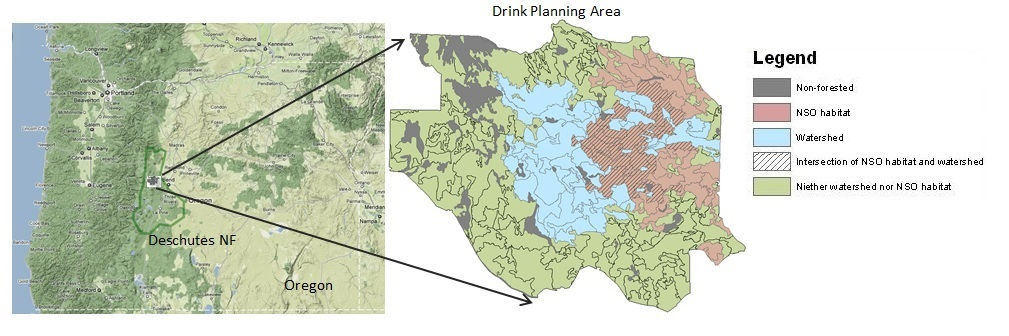
\includegraphics[width=.9\textwidth]{../images/Drink_Overview}
\caption[Overview of the study system, the Drink Planning Area]{Overview of the study system, the Drink Planning Area, consisting of 7056 ha in the Deschutes National Forest. The Drink Area contains old growth forest that make it suitable habitat for the northern spotted owl. It also houses the municipal watershed for Bend, OR and Sisters, OR.}
\label{fig:drinkOverview}
\end{figure}

\begin{figure}
\centering
\caption[Northern spotted owl]{The northern spotted owl is a threatened species whose habitat includes forests in the Pacific Northwest, including the Drink Area.}
\label{fig:nso}
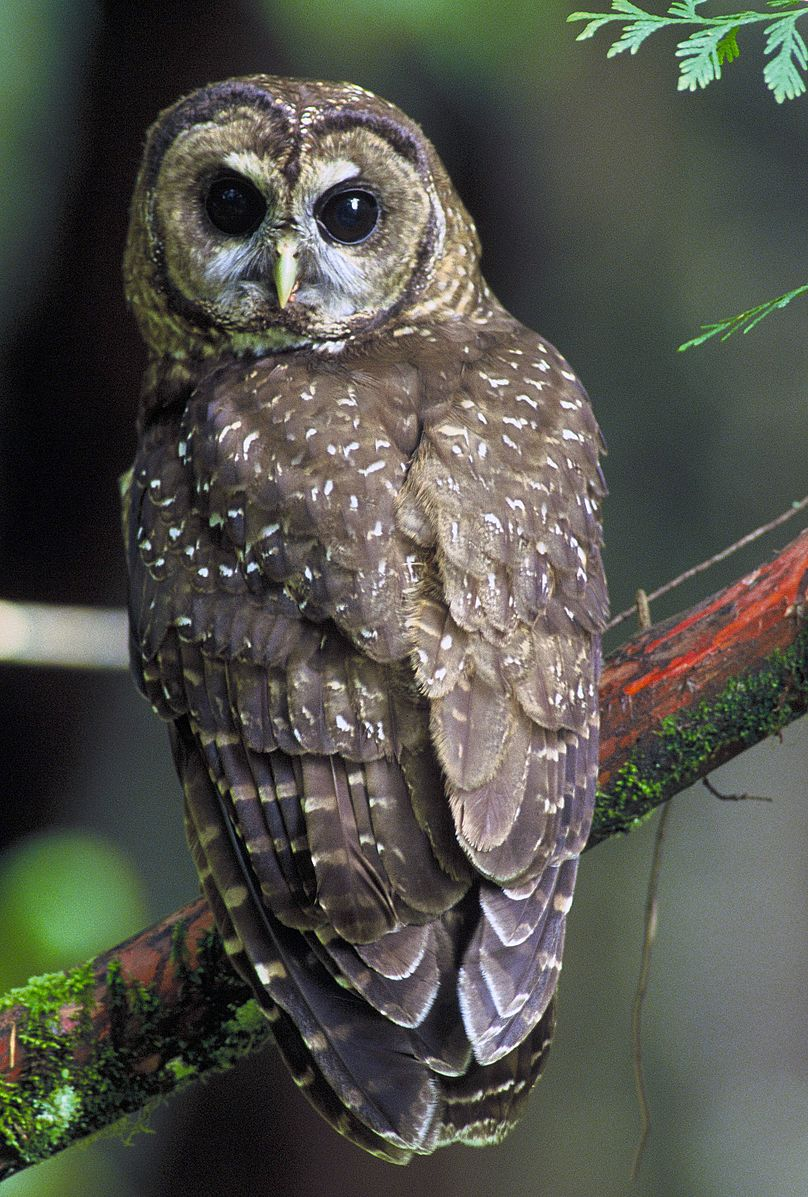
\includegraphics[width=.2\textwidth]{../images/NorthernSpottedOwl_USFWS}
\end{figure}

For these reasons, the managing entity, the United States Forest Service (USFS), would like to perform fuel removals in the Drink in order to reduce the area's fire hazard. However, performing these fuel removals has the potential to disrupt the habitat of the NSO \cite{bond2002short} and to induce short-term increases in sediment delivery \cite{o2005conceptual}. The latter is expected to be especially true in the Drink Area, where local USFS staff have noted that the watershed is unusually susceptible to spikes in sediment delivery as a result of foot traffic and other activities that occur within the watershed.

We developed a multi-objective mathematical program that optimizes the joint provision of these conflicting ecosystem services\footnote{These represent only a subset of the ecosystem services of concern to the USFS in the Drink Area. While the USFS manages for many ecosystem services simultaneously, many of the services are stacked rather than bundled, meaning the ecosystem services are not in conflict. These services need not all be considered in the multi-objective model, because the selection and maximization of one ecosystem service entails the maximization of all in the stack. For this reason, we have disregarded non-conflicting ecosystem services and selected a minimal bundle on which to employ multi-objective optimization. Those that do not conflict can be stacked post-optimization.}.

\subsection{The multi-objective model}
The multi-objective model is a zero-one mathematical program that assigns spatiotemporal prescriptions for fuel removals across the Drink Area to optimize the joint provision of ecosystem services. Spatially, the model prescribes fuel removals across 303 forest stands into which the Drink has been divided (the interior polygons in Figure \ref{fig:drinkOverview}). Temporally, the model operates over an 80-year planning horizon, from 2015 to 2095. The fuel removals are scheduled in two 20-year treatment periods: 2015-2035 and 2035-2055. For each stand, the model may prescribe fuel removals in the first period, the second period, neither, or both.

To ensure long-term efficacy of the fuel removals, the model minimizes the fire hazard rating of the Drink Area at the end of the 80-year planning horizon. To mitigate impacts of the fuel removals on NSO habitat, the model maximizes the area of NSO habitat at the end of each planning period. Similarly, the model minimizes the short-term spikes in sediment delivery resulting from the application of fuel removals, which are assumed to be performed at the midpoint year in the treatment periods (years 2025 and 2045). Figure \ref{fig:drinkPlanningHorizon} contains a schematic of the planning horizon which shows the timing of these events.

\begin{figure}
\centering
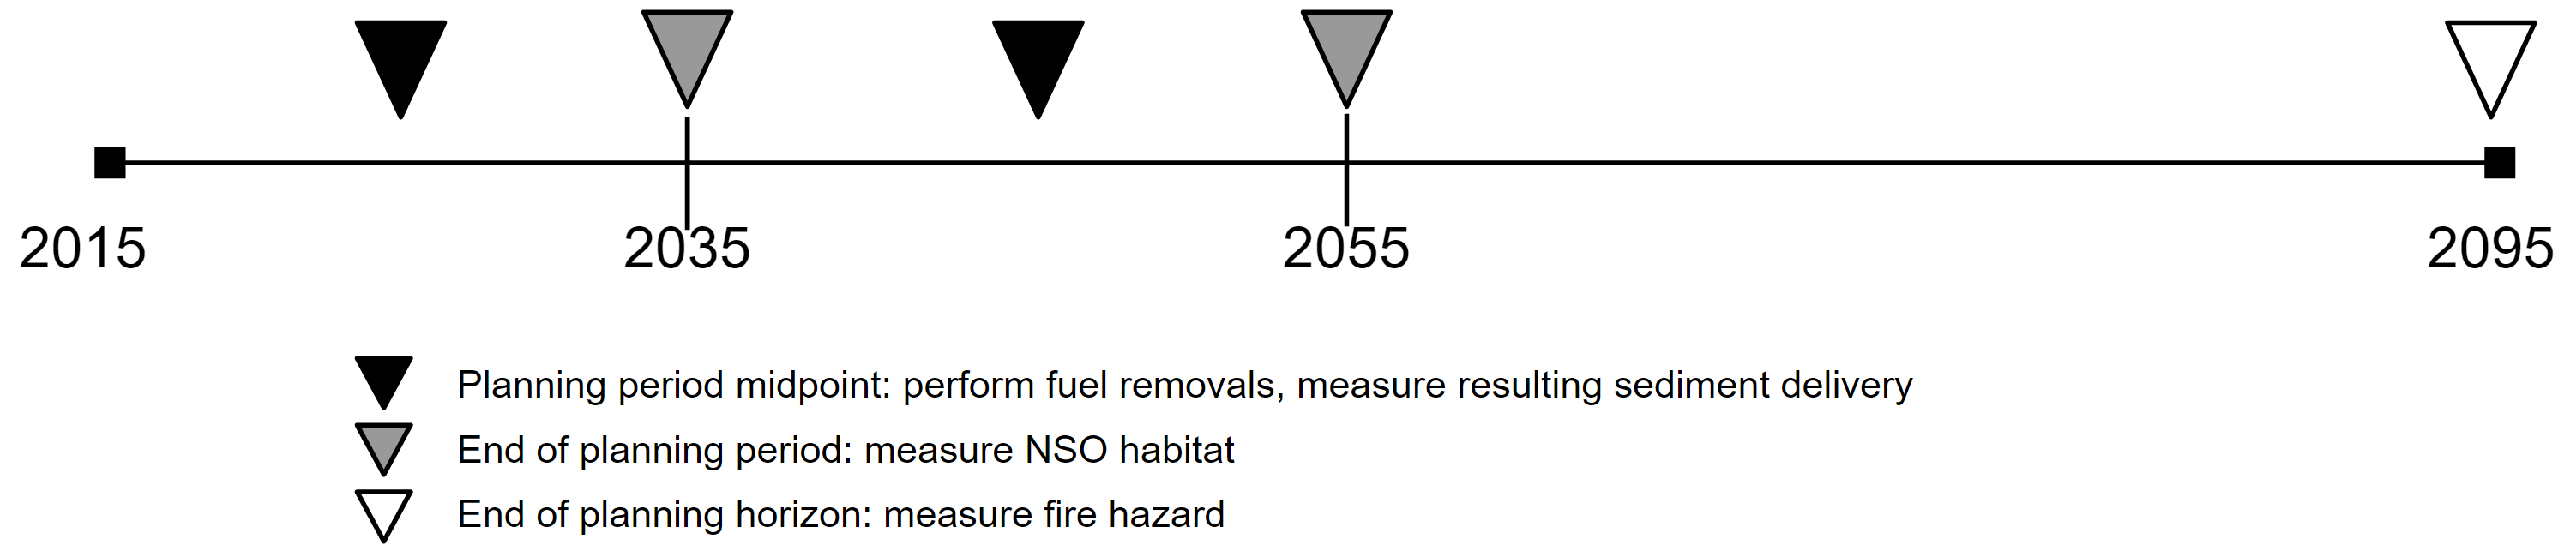
\includegraphics[width=.9\textwidth]{../images/Drink_PlanningHorizon_Sketch}
\caption[Planning horizon for the case study]{The planning horizon used in the case study spans the 80 year period from 2015 to 2095. Fuel removals may be performed in the first period (2015-2035), the second period (2035-2055), both, or neither. Fuel removals are assumed to be performed at the mid-point years of each period (black triangles). Sediment delivery is measured on treatment years. Stands' suitability for NSO habitat is measured at the end of the planning periods (gray triangles), and stands' fire hazard ratings are measured at the end of the planning horizon (white triangle).}
\label{fig:drinkPlanningHorizon}
\end{figure}

\subsubsection{Notation}
We use the following notation in the development of the model:

\paragraph{Model parameters}
\begin{itemize}
\item \textbf{$i \in I$:} the set of forest stands comprising the Drink Area ($|I| = 303$)

\item \textbf{$a_i$:} the area of stand $i$

\item \textbf{$r \in R$:} the set of fuel removal prescriptions:
	$$
	r =
	\begin{cases}
	1 &\text{ fuel removals in the first period (2015-2035)}\\
	2 &\text{ fuel removals in the second period (2035-2055)}\\
	3 &\text{ fuel removals in both periods}\\
	0 &\text{ no fuel removals performed in either period}
	\end{cases}
	$$
	
\item \textbf{$F_{i,r}$:} the area-weighted fire hazard rating of stand $i$ at the end of the planning horizon if prescribed to fuel removal schedule $r$. For instance, if a stand $i$ under fuel removal schedule $r$ has a fire hazard rating of 4 in the year 2095, and its area is 10 hectares, then $F_{i,r} = 40$. The metric for fire hazard rating used in this analysis was developed by Schroder \textit{et al.} \cite{schroder2016multi} specifically for the Drink Area. It uses fire characteristics from the set of fuel models proposed by Anderson \cite{anderson1982aids} in order to assign a fire hazard rating. We expand the rating system to include fuel models not present in Schroder \textit{et al.} See Table \ref{tab:firehazards} for the mapping of fuel models to fire hazard ratings.

The USFS's Climate-Forest Vegetation Simulator (Climate-FVS) was used to generate the fuels and vegetation characteristics of the stands in order to determine their fire hazard rating. Initial vegetation data for Climate-FVS came from the 2012 GNN structure map (\url{http://lemma.forestry.oregonstate.edu/data/structure-maps}) from Oregon State University's Landscape Ecology, Modeling, Mapping \& Analysis (LEMMA) group. Plots from the LEMMA database were mapped to the stands in the Drink area in order to produce tree and stand lists. These lists were used with Climate-FVS to simulate the stands' vegetation and fuels characteristics forward for the duration of the planning horizon under each climate scenario. Input climate data for Climate-FVS was obtained through the Climate-FVS climate data server \cite{climateFVSReadyData}.

\begin{table}[!ht]
\centering
\resizebox{\textwidth}{!}{%
\begin{tabular}{lccrrr}
\multicolumn{1}{c}{Fuel Model} & \multicolumn{1}{c}{\textbf{Fire Hazard Rating}} & \multicolumn{1}{c}{Group} & \multicolumn{1}{c}{Flame length (m)} & \multicolumn{1}{c}{Rate of spread (m/hr)} & \multicolumn{1}{c}{Total fuel load (tons/ha)} \\ \hline
4*                              & \textbf{5}                                       & Shrub                     & 5.79                                 & 1508.76                                   & 32.12                                         \\
5                               & \textbf{4}                                       & Shrub                     & 1.22                                 & 362.10                                    & 8.65                                          \\
8                               & \textbf{1}                                       & Timber                    & 0.30                                 & 32.19                                     & 12.36                                         \\
9*                              & \textbf{2}                                       & Timber                    & 0.79                                 & 150.88                                    & 8.65                                          \\
10                              & \textbf{2}                                       & Timber                    & 1.46                                 & 158.92                                    & 29.65                                         \\
11*                             & \textbf{2}                                       & Logging Slash             & 1.07                                 & 120.7                                     & 28.42                                         \\
12                              & \textbf{4}                                       & Logging Slash             & 2.44                                 & 261.52                                    & 85.50                                         \\
13                              & \textbf{5}                                       & Logging Slash             & 3.20                                 & 271.58                                    & 143.57                                       
\end{tabular}%
}
\caption[Fire hazard ratings used in multi-objective model]{Fire hazard rating system used here, originally employed by Schroder \textit{et al.} \cite{schroder2016multi}. Non-forested areas are assigned a fire hazard value of 0.\\
Asterisks (*) denote fuel models not present in Schroder \textit{et al.}\\
The fuel model column refers to the Anderson fuel model ratings \cite{anderson1982aids}.}
\label{tab:firehazards}
\end{table}

\item \textbf{$I_{\omega,t}$:} the set of stands that qualify as NSO habitat at the end of planning period $t$ under at least one fuel removal schedule. The stands that qualify as NSO habitat at the end of a planning period $t$ are those that meet the following three criteria in year $t$, as specified by the USFS:
	\begin{enumerate}
	\item elevation less than 1830 m
	\item the presence of trees with diameter at breast height (DBH) at least 76 cm
	\item canopy closure of at least 60\%
	\end{enumerate}
The elevation requirement was checked using a digital elevation model from the US Department of Agriculture's GeoSpatial Data Gateway; canopy closure and large tree criteria were determined using the simulated vegetation characteristics output from Climate-FVS.

In addition, to account for the large habitat requirements of the NSO, stands must be members of a cluster exceeding 200 ha in size, the entirety of which meets the aforementioned NSO habitat criteria. Stands that meet the first three criteria but are not part of such a cluster are less valuable NSO habitat and therefore have their contributions to the total owl habitat discounted by a factor of $e$.

\item \textbf{$e$:} the discount factor applied to NSO habitat when it is not part of a contiguous habitat cluster at least 200 ha in size. Following the convention used in Schroder \textit{et al.} \cite{schroder2016multi}, we set $e = 0.5$.

\item \textbf{$j \in R_{i,t}$:} the set of fuel removal schedules such that stand $i$ qualifies as NSO habitat at the end of planning period $t$. For instance, consider stand $i=15$ and planning period $t=2$ (2035-2055). We seek to find the set of fuel removal prescriptions $r \in R$ such that stand 15 is suitable NSO habitat at the end of planning period 2 (in year 2055). We enumerate the vegetation characteristics of stand 15 for all possible fuel removal schedules and determine that if fuel removals are assigned in the second planning period, then stand 15 does not qualify as NSO habitat in year 2055. Thus, $R_{15,2} = \{0,1\}$, since for $r=0$ (no fuel removals performed) and $r=1$ (fuel removals performed in first period only), stand 15 does qualify as NSO habitat in 2055.

\item \textbf{$s_{i,t}$:} the amount of sediment (in tonnes) delivered to the watershed as a result of performing fuel removals on stand $i$ in planning period $t$. The contributions of sediment delivery from treatment of stand $i$ in period $t$ were determined using the online GIS tool for the Watershed Erosion Prediction Project (WEPP) \cite{frankenberger2011development}. This tool takes soil textures, treatment types, duration of simulation, and custom climate data as inputs. Soil texture data for the Drink area was obtained from the USDA's Soil Survey Geographic (SSURGO) database, treatment types are those specified in \S \ref{chap:appendix_drinkTreatments}, and the years of simulation correspond to the treatment years in the planning horizon (2015-2095). The custom climate data are those described above for use with Climate-FVS, obtained through the Climate-FVS data server.

\item \textbf{$c \in C$:} Recall that the quantification of NSO habitat depends on the availability of large contiguous habitat patches; areas of NSO habitat less than than 200 ha in size are discounted. In order to determine when habitat is provided in sufficiently large areas, we must enumerate the set of clusters of stands whose combined area exceeds 200 ha. This set of clusters is the set $C$.

\item \textbf{$i \in D_c$:} Given a cluster $c \in C$, the set $D_c$ is the set of stands that comprise cluster $c$.

\item \textbf{$c \in C_i$:} Given a stand $i$, we define the set $C_i$ as the set of clusters that contain stand $i$

\item \textbf{$A$:} the maximum area in hectares that may be treated in either planning period. We constrain the allowable treatment area per period to account for the limited availability of work crews to perform the fuel removals. Following guidance from the USFS, we set $A = 2428$ ha (approximately 6000 ac).

\item \textbf{$\ell$, $u$:} the lower and upper bounds, respectively, on the relative fluctuation in the area treated in periods 1 and 2. These bounds are used to enforce regulation in the workflow for the USFS. Here we use values such that the area for which fuel removals are performed does not fluctuate more than 20\% between treatment periods; that is, we set the lower bound $\ell = 0.8$ and the upper bound $u = 1.2$.
\end{itemize}

\paragraph{Decision Variables}
$$
x_{i,r} = \begin{cases}
1 &\text{ if stand $i$ is prescribed to treatment schedule $r$}\\
0 &\text{ otherwise}
\end{cases}
$$ 

\paragraph{Indicator Variables}
\begin{itemize}
\item \textbf{$q_{c,t} = 1$} if all stands in cluster $c$ qualify as NSO habitat at the end of planning period $t$; $q_{c,t} = 0$ otherwise
\item \textbf{$p_{i,t} = 1$} if in planning period $t$ stand $i$ is part of a cluster $c$ such that $q_{c,t} = 1$; $p_{i,t} = 0$ otherwise
\end{itemize}

\paragraph{Accounting Variables}
\begin{itemize}
\item \textbf{$S_t$:} the total sediment delivered to the watershed from performing fuel treatments in planning period $t$
\item \textbf{$O_t$:} the amount of NSO habitat (in hectares) at the end of planning period $t$
\item \textbf{$H_t$:} the total area (in hectares) treated in planning period $t$
\end{itemize}

\subsubsection{Model formulation}
The formulation of the multi-objective model is as follows:
\begin{align}
Minimize \quad & \notag\\
&\sum_{i\in I}\sum_{r\in R} F_{i,r} x_{i,r} \label{eqn:objFire} \\
&\max \{S_1,S_2\} \label{eqn:objSediment} \\
Maximize \quad & \notag\\
&\min \{O_1,O_2\} \label{eqn:objOwl}
\end{align}
Subject to:
\begin{align}
\sum_{i\in I_{\omega,t}} \left(a_i p_{i,t} + e a_i \left( \sum_{j \in R_{i,t}} x_{i,j}-p_{i,t} \right) \right) &= O_t \qquad \forall t \in \{1,2\} \label{eqn:constraintDefOwl}\\
\sum_{i\in I} \sum_{r\in 1,3} s_{i,1} x_{i,r} &= S_1 \label{eqn:constraintSediment1} \\
\sum_{i\in I} \sum_{r\in 2,3} s_{i,2} x_{i,r} &= S_2 \label{eqn:constraintSediment2} \\
\sum_{i \in D_c} \sum_{j \in R_{i,t}} x_{i,j} - |c| q_{c,t} &\ge 0 \qquad \forall t \in \{1,2\}, c \in C \label{eqn:constraintClusterTriggers} \\
\sum_{c \in C_i} q_{c,t} - p_{i,t} &\ge 0 \qquad \forall t \in \{1,2\}, i \in I_{\omega,t} \label{eqn:constraintPVarTriggers} \\
\sum_{r \in R} x_{i,r} &= 1  \qquad \forall i \in I \label{eqn:constraintOnePrescrip} \\
\sum_{i \in I} \sum_{r \in 1,3} a_i x_{i,r} &= H_1 \label{eqn:constraintAreaAcctg1} \\
\sum_{i \in I} \sum_{r \in 2,3} a_i x_{i,r} &= H_2 \label{eqn:constraintAreaAcctg2} \\
H_t &\le A \qquad \forall t \in \{1,2\} \label{eqn:constraintAreaRestr} \\
\ell H_1 - H_2 &\le 0 \label{eqn:constraintAreaFlucL} \\
-u H_1 + H_2 &\le 0 \label{eqn:constraintAreaFlucU} \\
x_{i,r}, p_i, q_c \in \{0,1\} \quad &\forall i \in I, r \in R, c \in C \label{eqn:constraintNonNeg}
\end{align}

Equations \eqref{eqn:objFire}-\eqref{eqn:objOwl} are the objective functions: equation \eqref{eqn:objFire} minimizes the cumulative fire hazard rating of the Drink Area at the end of the 80-year planning horizon, equation \eqref{eqn:objSediment} minimizes the maximum peak in sediment delivery for the two planning periods, and equation \eqref{eqn:objOwl} maximizes the minimum NSO habitat available at the end of the planning periods. Equation set \eqref{eqn:constraintDefOwl} defines the amount of NSO habitat available at the end of the planning horizons. Note that if stand $i$ does not belong to a cluster of NSO habitat exceeding 200 hectares, then its area contribution to total NSO habitat is discounted by a factor of $e$. Equations \eqref{eqn:constraintSediment1} and \eqref{eqn:constraintSediment2} define the sediment delivered in planning periods one and two, respectively.

Inequality set \eqref{eqn:constraintClusterTriggers} controls the value of the cluster variables $q_{c,t}$ indicating clusters that meet the NSO habitat criteria in each of the planning periods. Inequality set \eqref{eqn:constraintPVarTriggers} controls the value of the $p_{i,t}$ variables indicating whether stand $i$ is included in a cluster of NSO habitat at time $t$.

The set of equalities \eqref{eqn:constraintOnePrescrip} enforces the logical constraint that each stand must be prescribed to exactly one fuel removal schedule. Equations \eqref{eqn:constraintAreaAcctg1} and \eqref{eqn:constraintAreaAcctg2} are accounting constraints for the total area treated in each planning period, and inequalities \eqref{eqn:constraintAreaRestr} ensure that this area does not exceed the predefined maximum. Inequalities \eqref{eqn:constraintAreaFlucL} and \eqref{eqn:constraintAreaFlucU} bound the fluctuation in treated area between the planning periods. Finally, constraint \eqref{eqn:constraintNonNeg} defines the decision and indicator variables as binary.

\subsection{Solution method}
We developed an implementation of T\'{o}th's Alpha-Delta algorithm \cite{TothThesis} to solve the model \eqref{eqn:objFire}-\eqref{eqn:constraintNonNeg} utilizing the IBM ILOG CPLEX optimization engine. For a problem with $M$ objectives, the Alpha-Delta algorithm finds the Pareto frontier by iteratively slicing the $M$-dimensional objective space with a tilted $M-1$-dimensional hyperplane. The algorithm was implemented using an alpha parameter of $\alpha = .01$ and delta parameters of $\delta_{Hab} = 1$ ha and $\delta_{Sed} = 2$ tonnes for the NSO habitat and sediment delivery objectives, respectively.

\subsection{Climate change scenarios}
\label{sec:climateChange}
Like other ecosystems, forests will undergo changes as a result of the changing climate. For instance, researchers anticipate new spatial distributions of tree species \cite{iverson1998predicting}, increased sediment delivery to streams \cite{Goode20121}, and increasing disturbance regimes such as wildfires, droughts, and insect infestations \cite{vose2012effects}. As these transformations occur, the ability of forests to provide ecosystem services will change.

The extent of change will likely depend on the severity of the realized climate change. Thus, to understand the potential impacts on ecosystem services, multiple climate change scenarios representing a range of severities should be considered. We use three in our case study: one scenario in which climate change is ignored, ``None''; one in which climate change is predicted to be mild, ``Ensemble RCP 4.5'' (also ``E45''); and one in which climate change is predicted to be severe, ``Ensemble RCP 8.5'' (also ``E85''). These scenarios differ in their assumption of the additional energy per unit area that will be absorbed by the atmosphere, a value known as radiative forcing (RF). E45 assumes an RF of 4.5 $W/m^2$ and E85 assumes 8.5 $W/m^2$. In general, larger values of RF correspond to more severe climate change.

A given value of radiative forcing does not map to a single prediction of climate change, because researchers may disagree in how the climate will respond to that amount of RF. This is why for a given RF numerous climate models exist. A common approach to handling the disagreement among the climate models is to use an ensemble of climate models that all assume the same RF. We adopt this approach here for our E45 and E85 scenarios.

Each of these scenarios corresponds to an ensemble of 17 climate models. These climate models originate from the Fifth Assessment (AR5) on climate performed by the Intergovernmental Panel on Climate Change (IPCC). The selection and assembly of the 17 climate models used in these ensembles was conducted by Cookston (2016) and the Climate-FVS team \cite{ClimateModelsInFVSEnsemble}.

The other scenario, None, ignores any effects of climate change. While the number of studies incorporating climate change is increasing, this is still a common assumption in modern studies such as Schroder \textit{et al}. (2013) \cite{schroder2016multi}. Because it has served as the basis for many past studies of ecosystem services, the None climate scenario serves as a control against which we will compare the other two.

Each climate scenario corresponds to a different parameterization of the model, since the vegetation, fuels, and sediment delivery data depend on climate. Thus, changing the climate scenario has the potential to affect the amount and location of NSO habitat, the effects of fuel removals on NSO habitat, the fire hazard of the Drink Area, the efficacy of the fuel removals in reducing fire hazard, and the sediment delivered as a result of fuel removals. This drives changes to the relationships among the ecosystem services as well, which we investigate using the aforementioned conflict measures.


\subsection{Results}
We parameterized and solved the multi-objective model (equations \eqref{eqn:objFire}-\eqref{eqn:constraintNonNeg}) for each of the climate scenarios, generating three efficient frontiers: $Z_{\text{None}}$, $Z_{E45}$, and $Z_{E85}$ for the None, Ensemble RCP 4.5, and Ensemble RCP 8.5 scenarios, respectively.  $Z_{\text{None}}$ consists of 51 solutions, $Z_{\text{E45}}$ consists of 701 solutions, and $Z_{\text{E85}}$ consists of 1083. Figure \ref{fig:frontiersAll} shows the frontiers in their 3-dimensional objective spaces while Figure \ref{fig:frontiersPCPlot} provides a single parallel coordinates plot with all frontiers. The summary details of their objective achievements are listed in Table \ref{tab:frontiersSummary}.

\begin{table}[]
\centering
\caption[Summary of objective achievement across climate scenarios]{Summary of the performance of the efficient frontiers for each climate change scenario.}
\label{tab:frontiersSummary}
\begin{tabular}{lllll}
\multicolumn{2}{l}{}                                                  & \textbf{None} & \textbf{E45} & \textbf{E85} \\ \hline
\multirow{3}{*}{\begin{tabular}[c]{@{}l@{}}\textbf{Fire hazard (cumulative}\\ \textbf{area-weighted fire hazard)}\end{tabular}}       & \multicolumn{1}{l}{min} & 21,321.21      & 23,219.82     & 23,268.02     \\
                                            & \multicolumn{1}{l}{avg} & 21,406.26      & 23,324.41     & 23,369.57     \\
                                            & \multicolumn{1}{l}{max} & 21,933.29      & 23,973.79     & 23,724.98     \\ \hline
\multirow{3}{*}{\textbf{NSO habitat (ha)}}       & \multicolumn{1}{l}{min} & 2,532.33       & 2,412.18      & 2,171.10      \\
                                            & \multicolumn{1}{l}{avg} & 2,536.31       & 2,447.92      & 2,421.99      \\
                                            & \multicolumn{1}{l}{max} & 2,540.05       & 2,477.18      & 2,481.01      \\ \hline
\multirow{3}{*}{\textbf{Sediment delivery (tonnes)}} & \multicolumn{1}{l}{min} & 0             & 0            & 0            \\
                                            & \multicolumn{1}{l}{avg} & 10.25         & 27.98        & 31.19        \\
                                            & \multicolumn{1}{l}{max} & 24.57         & 63.43        & 69.68        
\end{tabular}
\end{table}


\begin{figure}[ht!]
  \subfloat[None]{%
    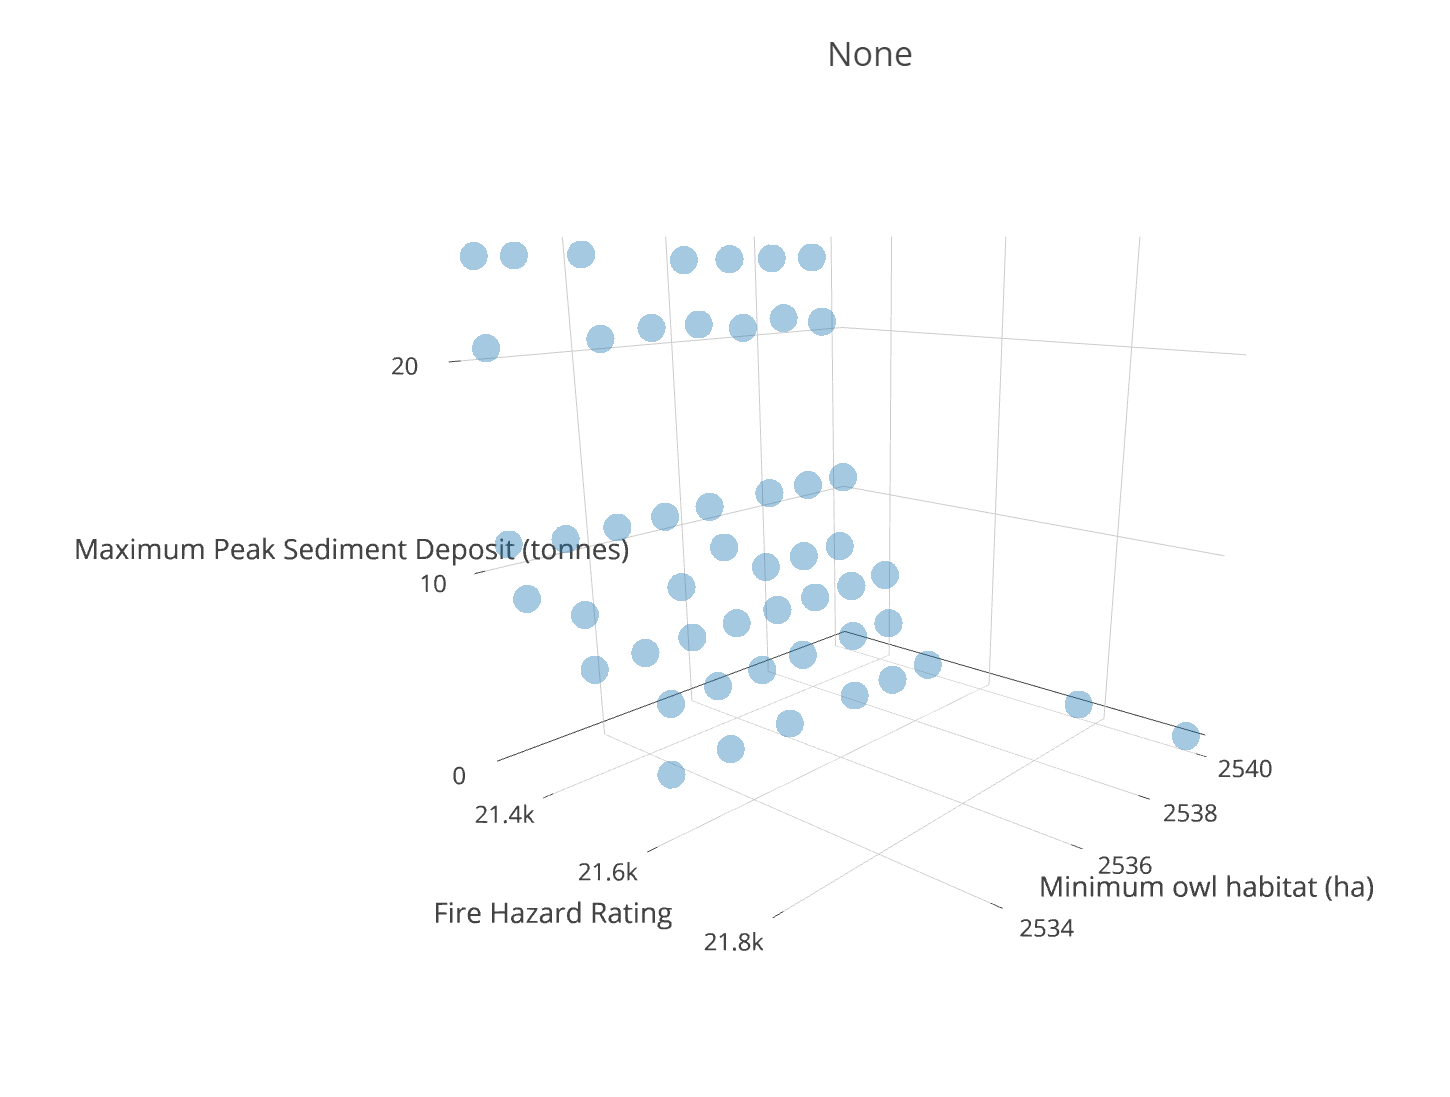
\includegraphics[width=.49\textwidth]{../images/Frontier_None}%
    \label{fig:frontierNone}%
  }
  \subfloat[Ensemble RCP 4.5]{%
    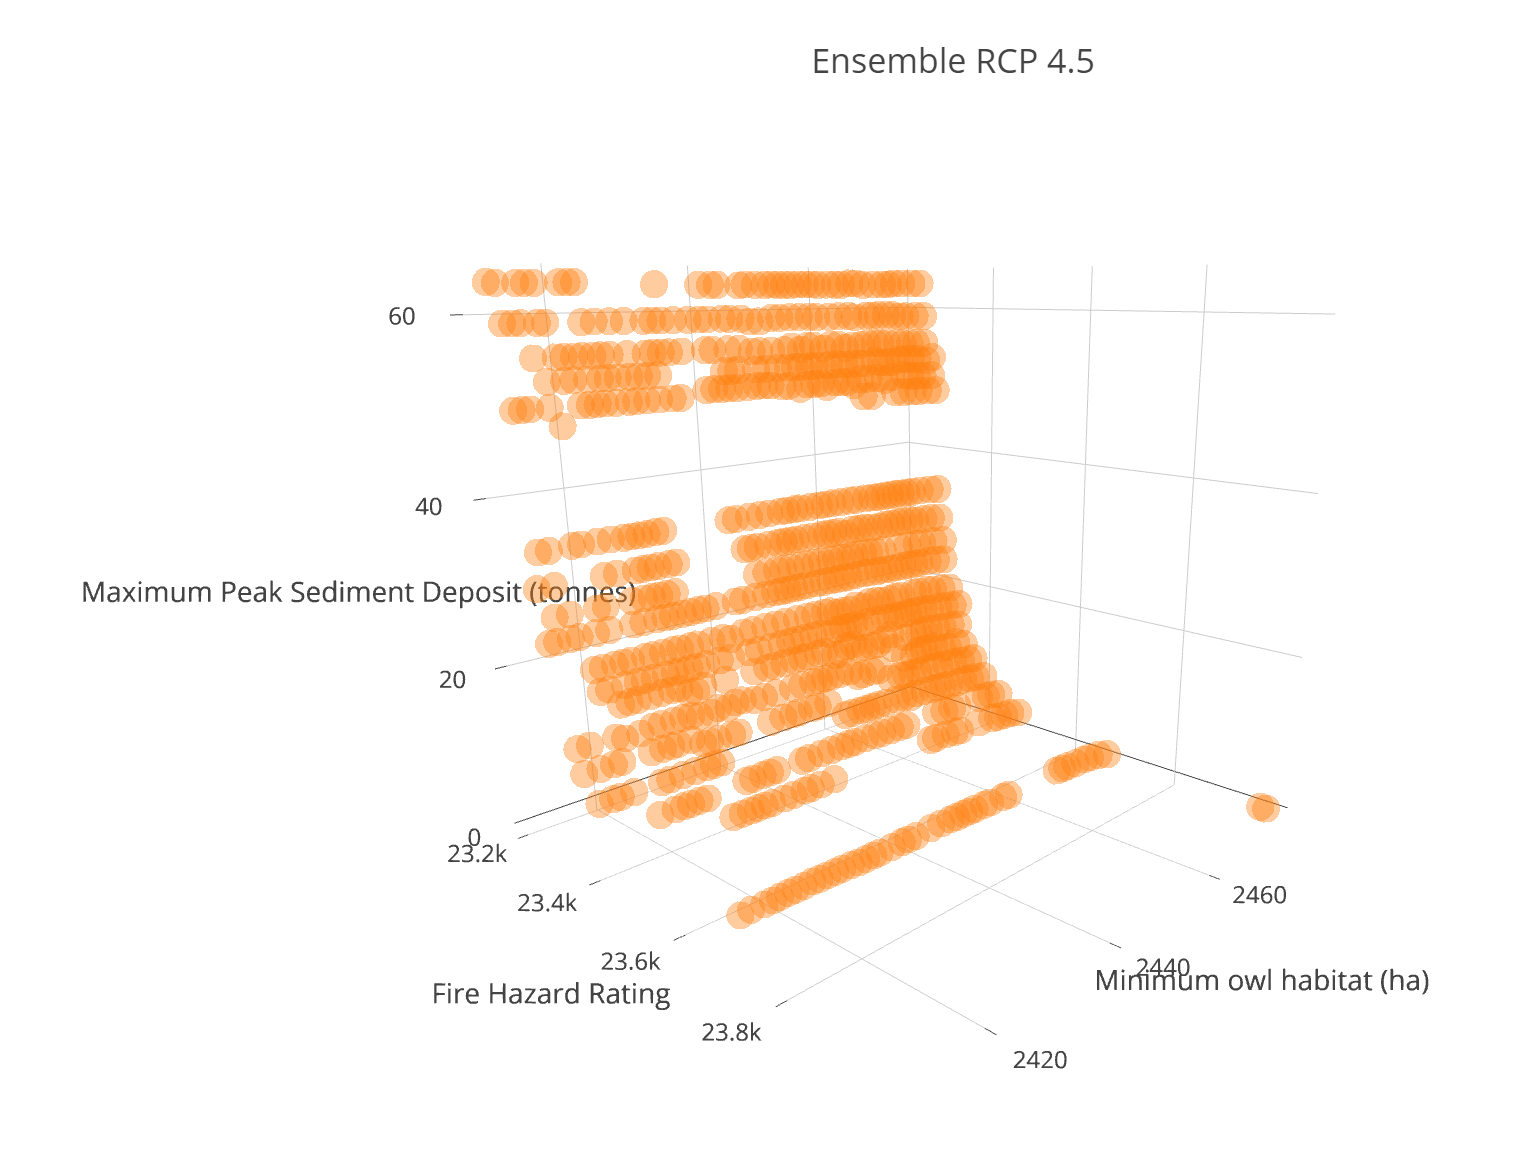
\includegraphics[width=.49\textwidth]{../images/Frontier_E45}%
    \label{fig:frontierE45}%
  }\hfill\centering
  \subfloat[Ensemble RCP 8.5]{%
    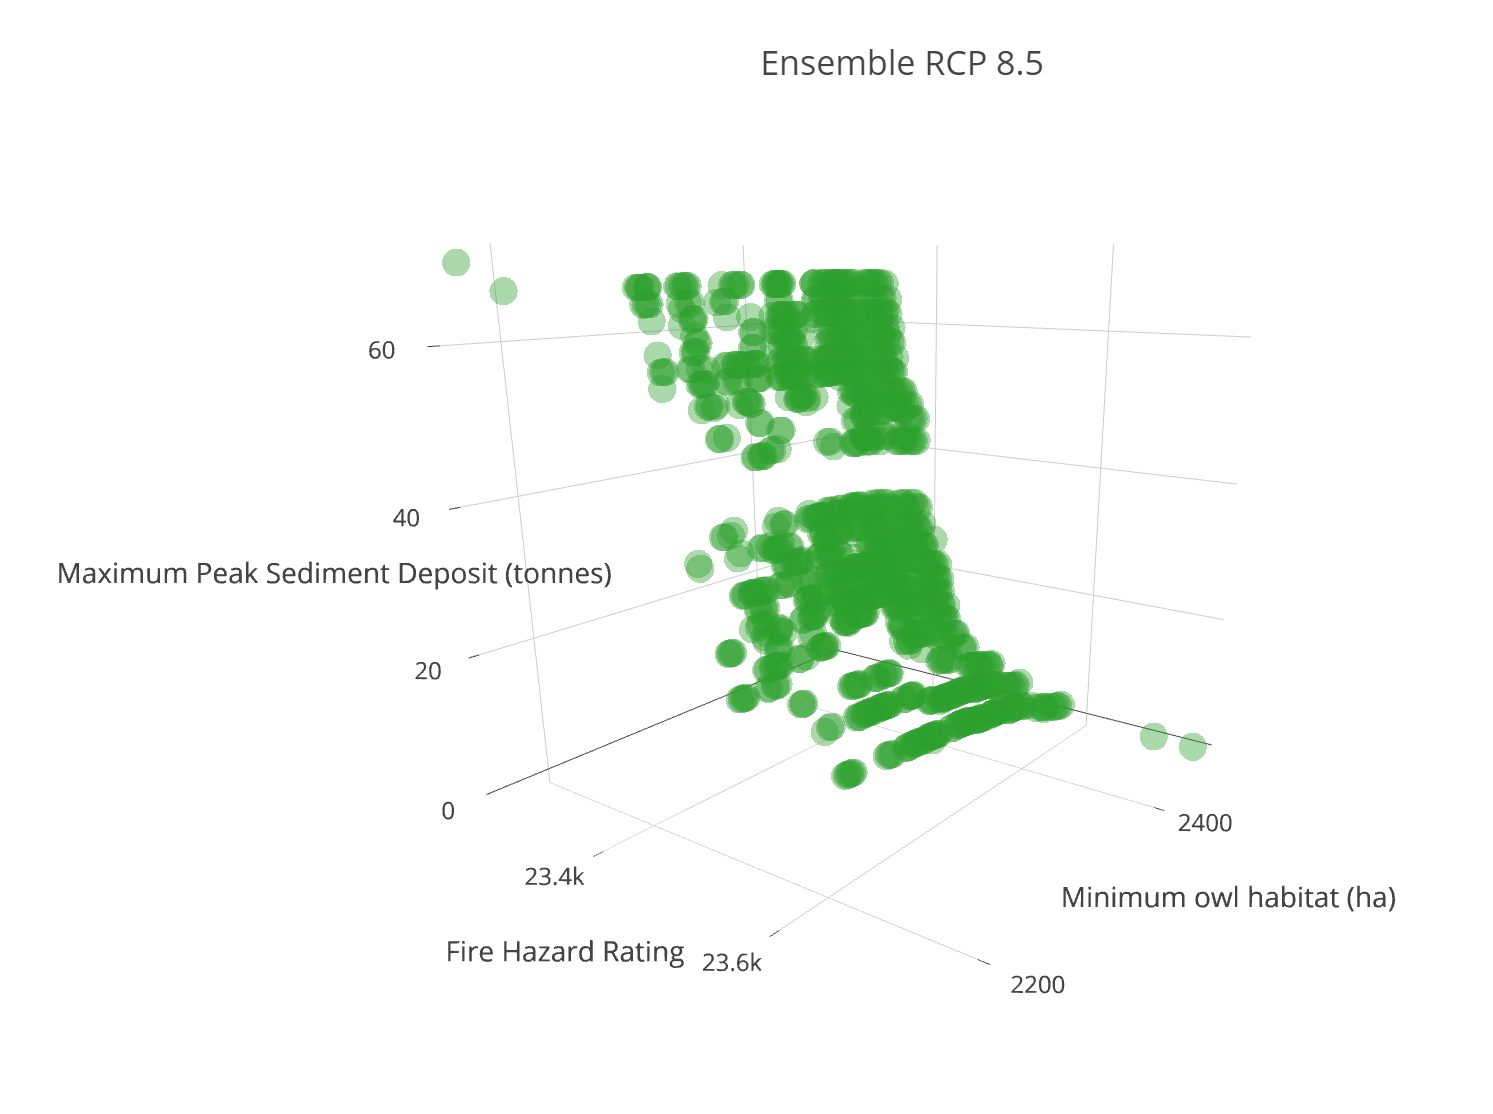
\includegraphics[width=.49\textwidth]{../images/Frontier_E85}%
    \label{fig:frontierE85}%
  }
  \caption[Frontiers for each climate change scenario]{Efficient frontiers for each climate change scenario.}
  \label{fig:frontiersAll}
\end{figure}

\begin{figure}[ht]
\centering
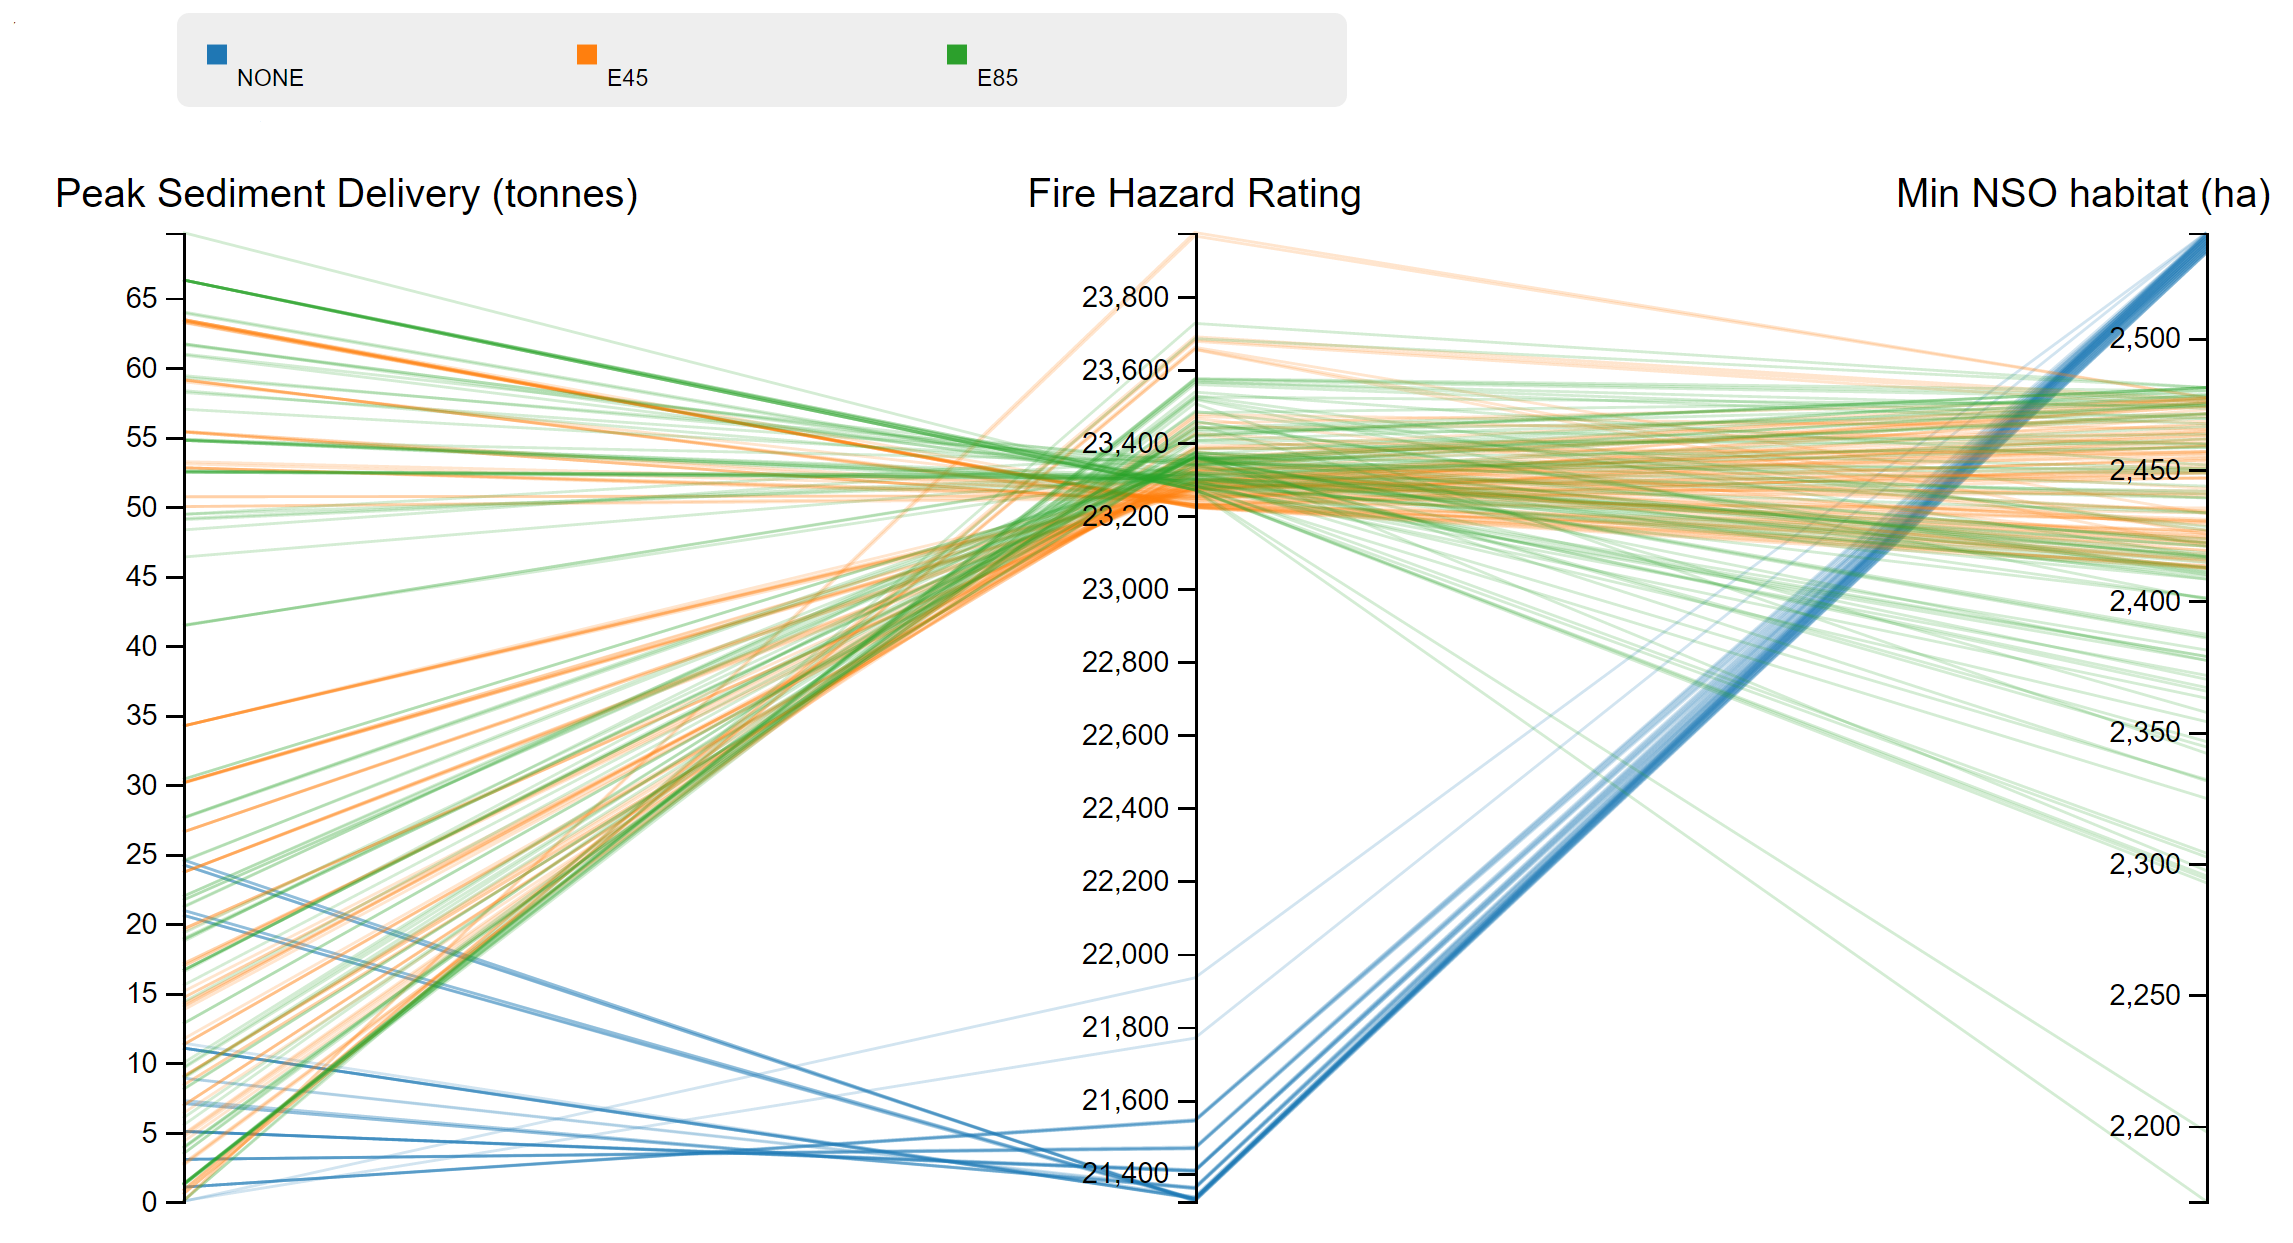
\includegraphics[width=.85\textwidth]{../images/FrontiersPCPlot}
\caption[Parallel coordinates view of the three frontiers]{Parallel coordinates view of the frontiers. Each axis represents an ecosystem service optimized by the model and each line represents a solution. In all objectives, we notice that None appears to outperform both the E45 and E85 scenarios, which show similar average objective achievements. To increase visual clarity, only a subset of solutions for E45 and E85 are shown.}
\label{fig:frontiersPCPlot}
\end{figure}

%We first report the impacts of climate change on the provision of individual ecosystem services before analyzing its impacts on the joint provision of ecosystem services and the conflict among them.

\subsubsection{Individual provision of ecosystem services}
The average achievement of all ecosystem services decreases with increasing severity of climate change -- see Table \ref{tab:frontiersSummary}. We find that the difference in ecosystem service provision is greater between the assumption of no climate change and mild climate change (None to E45) than it is between mild climate change and severe climate change (E45 to E85).

\paragraph{Sediment delivery} 
All scenarios have a lower bound on sediment delivery of 0, but the upper bound and the average sediment delivery both increase with climate change severity. Compared to the None scenario with an average sediment delivery of 10.25 tonnes, the average amount of sediment delivered in E45 is 27.98 tonnes, an increase of 172\%. The average for E85 is 31.19 tonnes, 204\% higher than None.

\paragraph{Fire hazard}
Similarly, we find that the average fire hazard of the Drink Area increases with climate change severity. The average for None is 21406.26 while E45 and E85 both perform approximately 9\% worse with an average of 23324.41 and 23369.57, respectively.

\paragraph{NSO habitat}
Finally, we also observe a decrease in the average provision of NSO habitat with increasing climate change. Compared to None which has an average provision of 2536.31 ha of NSO habitat, the average provision in the E45 scenario is 88.4 ha less (-3.5\%), and E85 is 114.3 ha less (-4.5\%).

We also find that for the sediment delivery and NSO habitat objectives, the range of achievable values increases with climate change severity. For sediment delivery, the range increases from 24.57 tonnes in None to 63.43 in E45 to 69.68 in E85. And for NSO habitat, the range increases from 7.72 ha in None to 65 ha in E45 and to 309.91 ha in E85.

\subsubsection{Conflict and the joint provision of ecosystem services}
As we saw for provision of individual ecosystem services, our results show that climate change will have an impact on conflict and the joint provision of ecosystem services as well.

We observe a decreasing hypervolume with increasing severity of climate change -- see Table \ref{tab:hypervols}. The hypervolume for E45 is $0.0101$ less than None, and E85 is $0.0474$ less than None. However, all hypervolumes indicate frontiers which fill a large percentage of the objective space, as the smallest value (E85) is $I_{H1}(Z_\text{E85}) = 0.8295$. The binary hypervolumes (see Table \ref{tab:binaryHypervols}) tend to align with the hypervolumes, with larger values of $I_{H2}(Z_1,Z_2)$ when $I_{H1}(Z_1) > I_{H1}(Z_2)$ and smaller values when $I_{H1}(Z_2) > I_{H1}(Z_1)$. We note that no frontier is dominated by any other, as all values in Table \ref{tab:binaryHypervols} are strictly positive.

\begin{table}[]
\centering
\caption[Hypervolumes of the efficient frontiers]{Hypervolume for each climate change scenario. Hypervolume values increase with increasing severity of climate change.}
\label{tab:hypervols}
\begin{tabular}{lllll}
\multicolumn{2}{l}{}                                                  & \textbf{None} & \textbf{E45} & \textbf{E85} \\ \hline
\multicolumn{2}{l}{\textbf{Hypervolume}}                              & 0.876977      & 0.866857     & 0.829541       
\end{tabular}
\end{table} 

\begin{table}[]
\centering
\caption[Binary hypervolume values for each pair of climate scenarios]{Binary hypervolumes for each pair of climate scenarios. No values are negative, indicating that no frontiers are dominated by another and that all frontiers uniquely enclose some volume of the objective space.}
\label{tab:binaryHypervols}
\begin{tabular}{lll}
\textbf{$Z_1$} & \textbf{$Z_2$} & \textbf{$I_{H2}(Z_1,Z_2)$} \\ \hline
\textbf{None}  & \textbf{E45}   & 0.026154                   \\
\textbf{None}  & \textbf{E85}   & 0.058001                   \\
\textbf{E45}   & \textbf{None}  & 0.016034                   \\
\textbf{E45}   & \textbf{E85}   & 0.045156                   \\
\textbf{E85}   & \textbf{None}  & 0.010565                   \\
\textbf{E85}   & \textbf{E45}   & 0.007841                  
\end{tabular}
\end{table}

\paragraph{Sediment delivery-NSO Habitat}
In the pairwise comparison of objectives, we observe little conflict between sediment delivery and NSO habitat under all climate scenarios. This is evident first in the proposed conflict metric $C_{ij}$, for which the largest value across all frontiers is 0.25 -- see Table \ref{tab:pairConflict-SedNSO}. We also notice the lack of conflict in Figure \ref{fig:pairplotNSOSed}. The figure shows the efficient frontier plotted in the sediment delivery-NSO habitat plane, where each objective has been normalized such that better values are higher and worse values are lower. For instance, in this graph, the point $(1,1)$ represents 0 sediment delivery and maximum NSO habitat. For all climate scenarios, we see similar uniform spreads of solutions as well as multiple solutions near the sub-dimensional ideal solution at $(1,1)$.

\begin{table}[]
\centering
\caption[Sediment-NSO conflict across climate scenarios]{Conflict between sediment delivery and NSO habitat across climate scenarios.}
\label{tab:pairConflict-SedNSO}
\begin{tabular}{llll}
\textbf{}     & \textbf{$C_{ij}$} & \textbf{$c_{ij,\rho}$} & \textbf{$c_{ij,d}$} \\ \hline
\textbf{None} & 0.19639           & 0.3974                 & 0.4942              \\
\textbf{E45}  & 0.25667           & 0.5194                 & 0.4941              \\
\textbf{E85}  & 0.19284           & 0.5160                 & 0.3737             
\end{tabular}
\end{table}


\begin{figure}[ht]
\centering
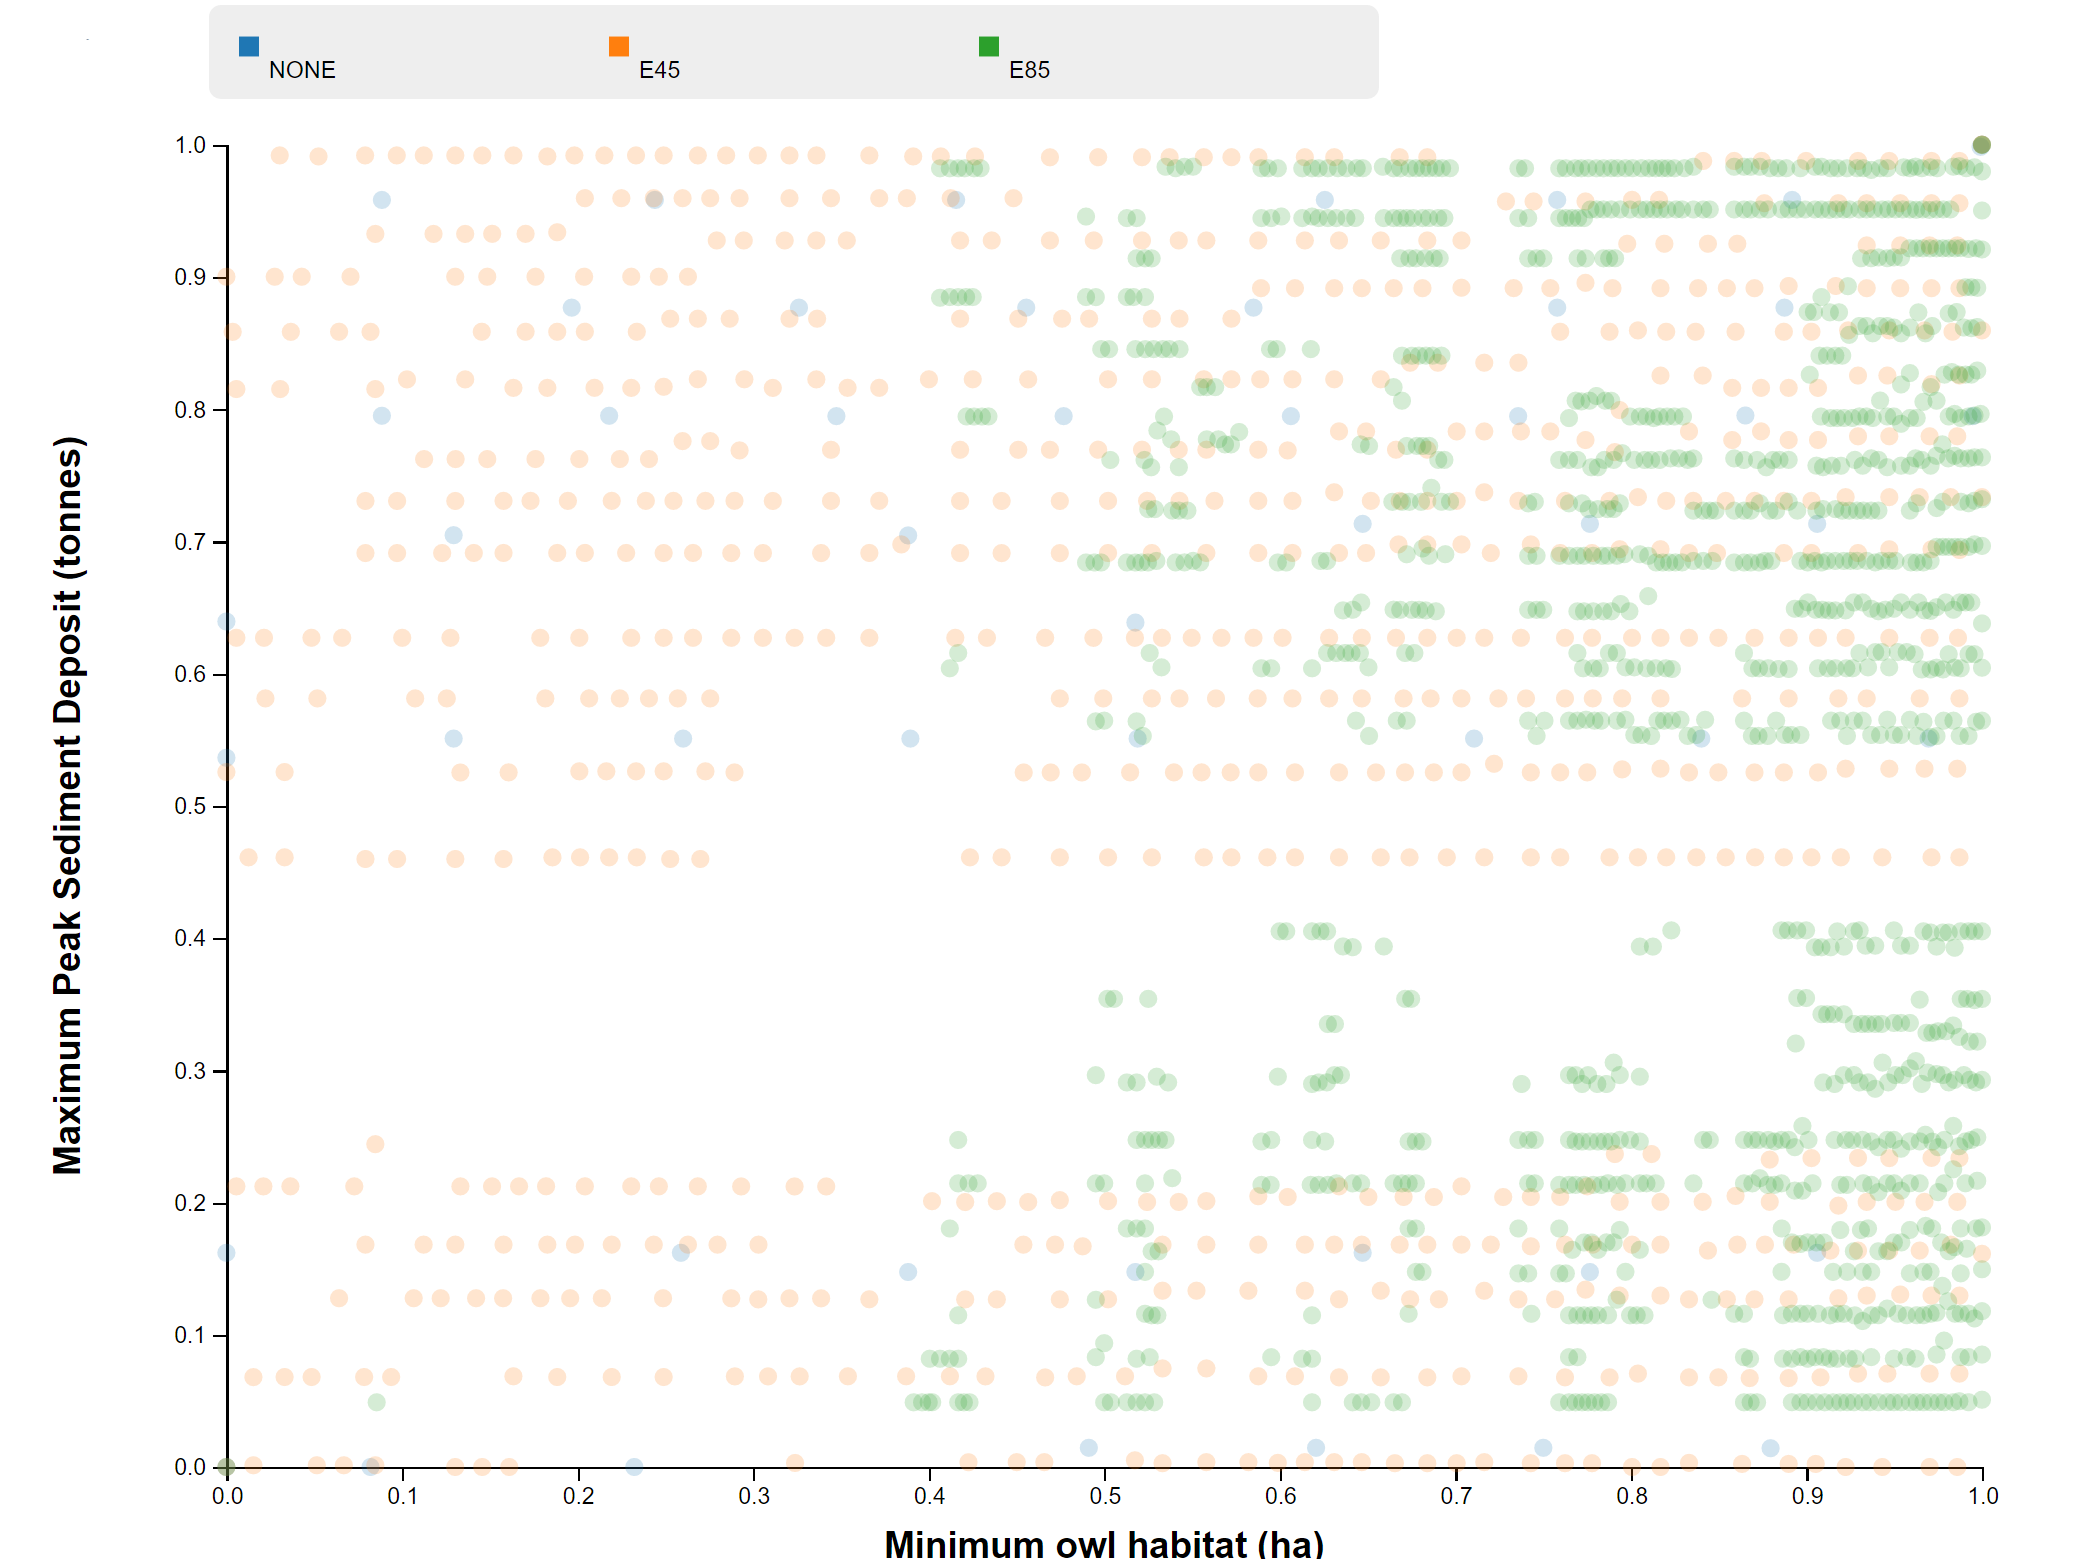
\includegraphics[width=.75\textwidth]{../images/2DSlice_NSO_Sed}
\caption[NSO habitat vs. sediment delivery for all climate scenarios]{NSO habitat versus sediment delivery for all climate scenarios. No obvious conflict pattern exists between the objectives in any climate scenario.}
\label{fig:pairplotNSOSed}
\end{figure}

\paragraph{NSO habitat-fire hazard}
According to $C_{ij}$, the conflict between NSO habitat and fire hazard is again small for all climate scenarios; however, it appears to decrease with increasing severity of climate change. We see in Table \ref{tab:pairConflict-NSOFire} that the average distance to the ideal decreases with increasing severity of climate change. See also Figure \ref{fig:pairplotNSOFire} which shows spreads of solutions for each climate scenario in the NSO habitat-fire hazard plane. The solutions are increasingly more clustered near the sub-dimensional ideal solution with increasing climate change severity.

\begin{figure}[ht]
\centering
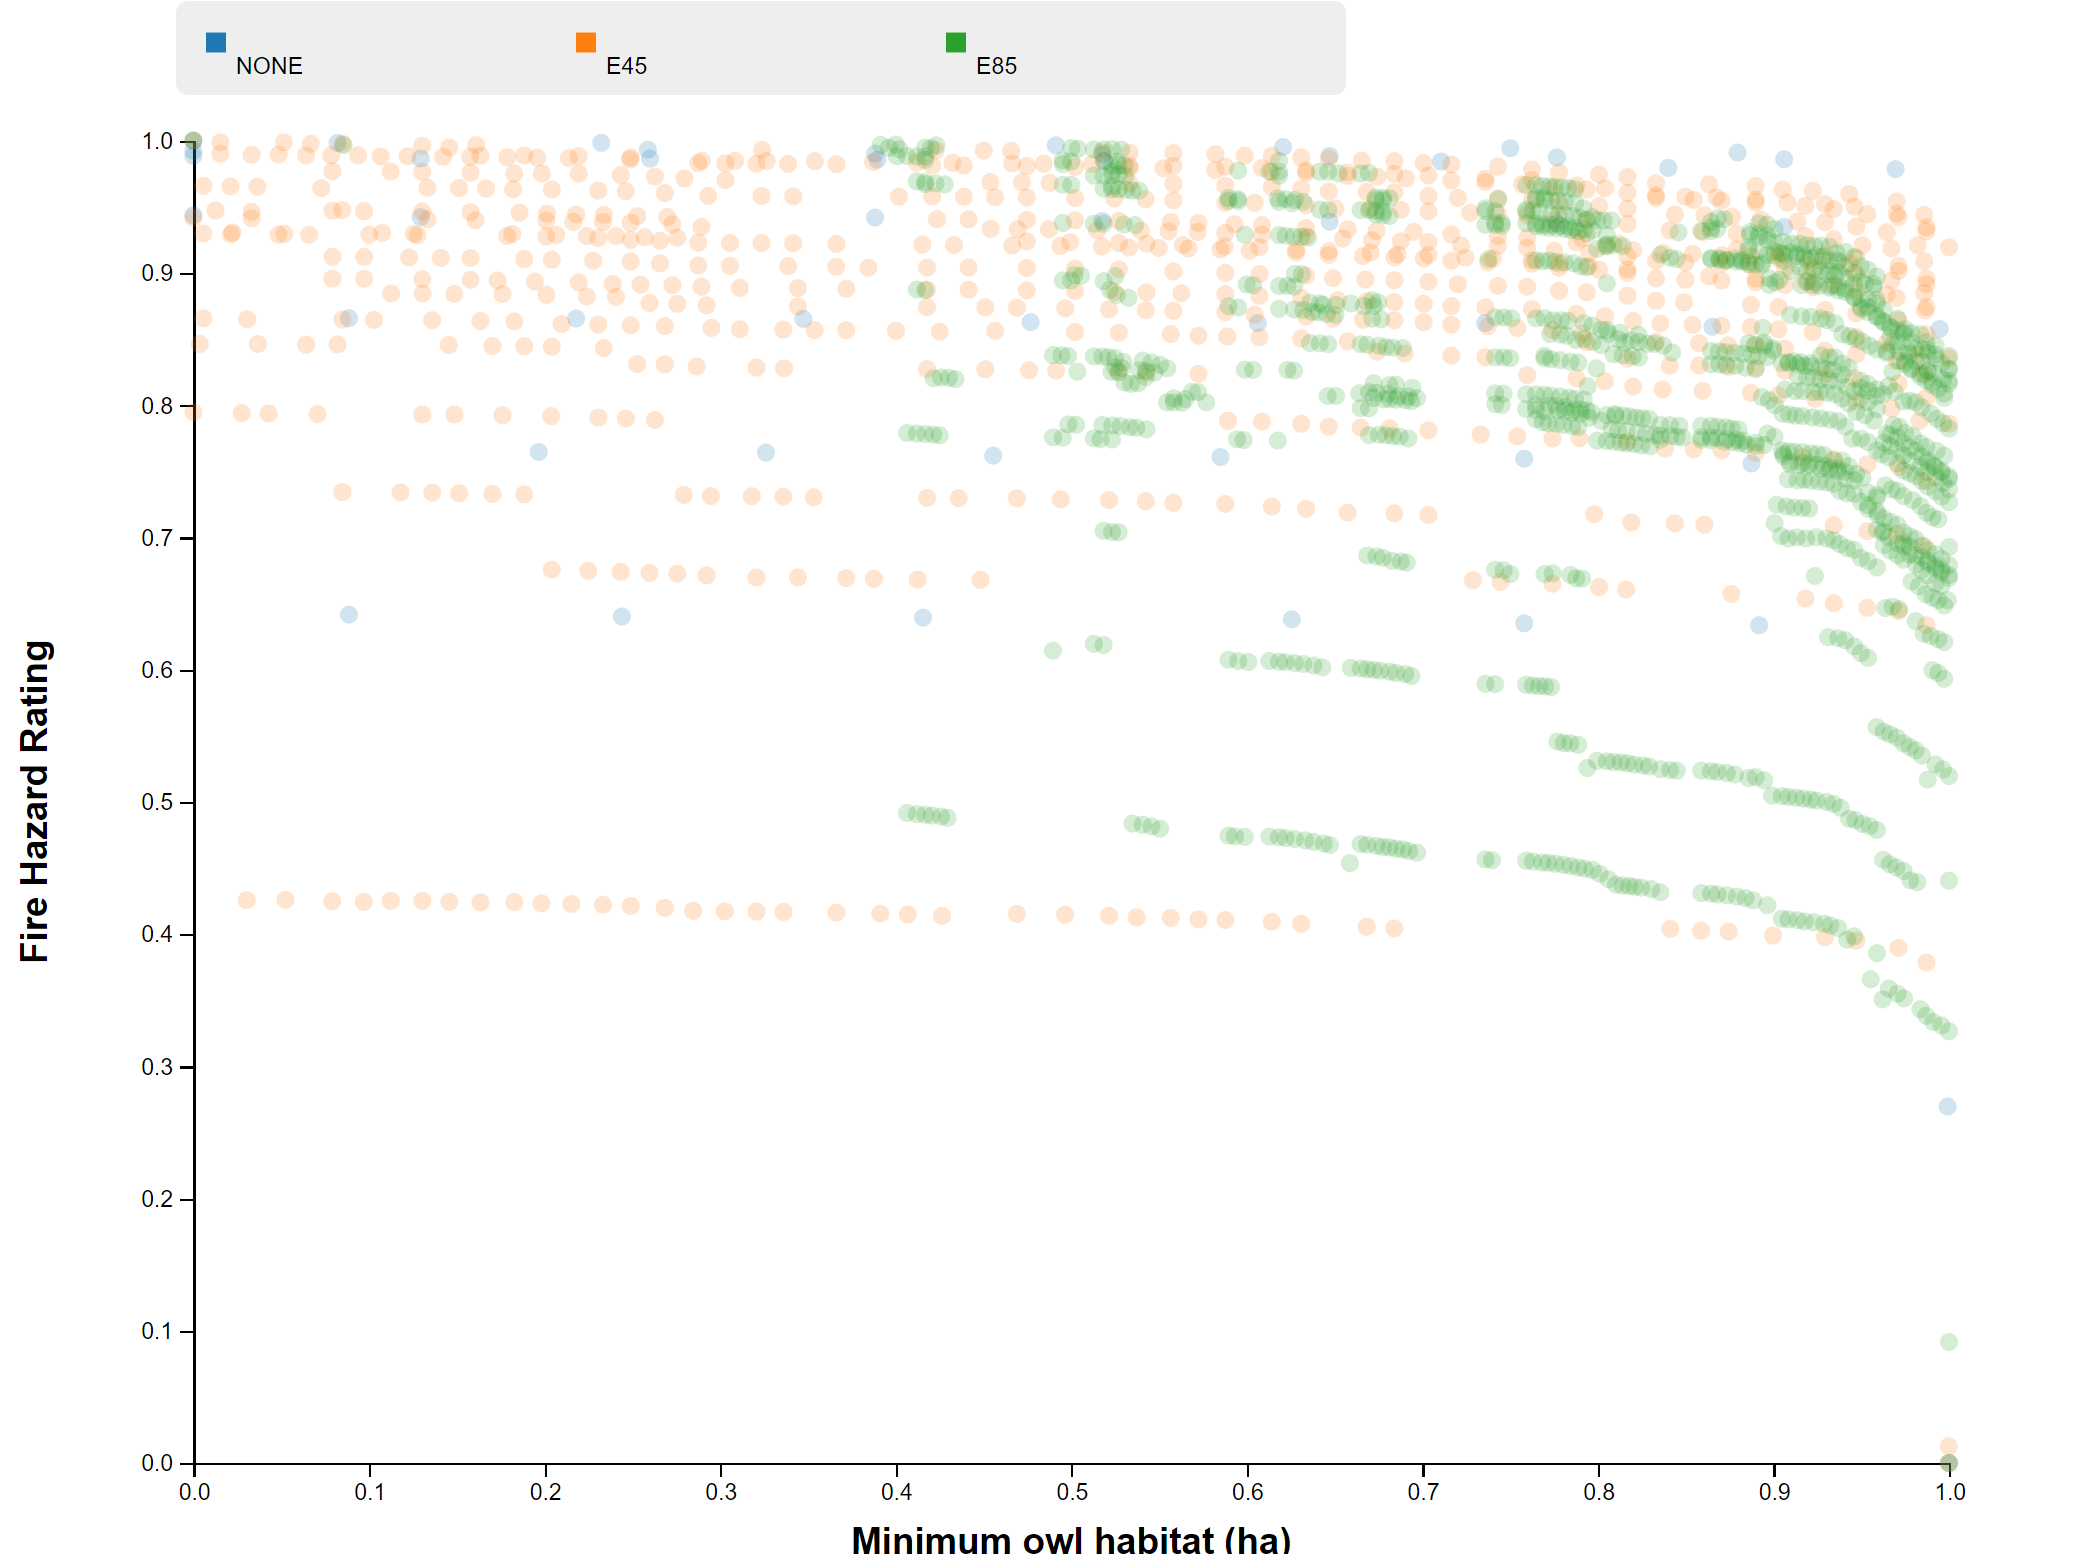
\includegraphics[width=.75\textwidth]{../images/2DSlice_NSO_Fire}
\caption[NSO habitat vs. fire hazard for all climate scenarios]{NSO habitat versus fire hazard for all climate scenarios.}
\label{fig:pairplotNSOFire}
\end{figure}

\begin{table}[]
\centering
\caption[NSO-fire hazard conflict across climate scenarios]{Conflict between NSO habitat and fire hazard across climate scenarios.}
\label{tab:pairConflict-NSOFire}
\begin{tabular}{llll}
\textbf{}     & \textbf{$C_{ij}$} & \textbf{$c_{ij,\rho}$} & \textbf{$c_{ij,d}$} \\ \hline
\textbf{None} & 0.25805           & 0.6622                 & 0.3897              \\
\textbf{E45}  & 0.20560           & 0.5807                 & 0.3541              \\
\textbf{E85}  & 0.15670           & 0.6643                 & 0.2359
\end{tabular}
\end{table}

\paragraph{Fire hazard-sediment delivery}
In all climate scenarios, the strongest pairwise conflict is between fire hazard and sediment delivery. This is apparent from both Figure \ref{fig:pairplotSedFire} and the conflict metric, Table \ref{tab:pairConflict-SedFire}. All rank correlation conflict values $c_{ij,\rho} > 0.95$, indicating strong negative rank correlation. In Figure \ref{fig:pairplotSedFire} we observe a clear void of solutions in all climate change scenarios near the sub-dimensional ideal solution at $(1,1)$; this is unlike Figures \ref{fig:pairplotNSOSed} and \ref{fig:pairplotNSOFire}. We also notice that the None and E45 solutions generally extend beyond the E85 solutions in this plane.

\begin{figure}[ht]
\centering
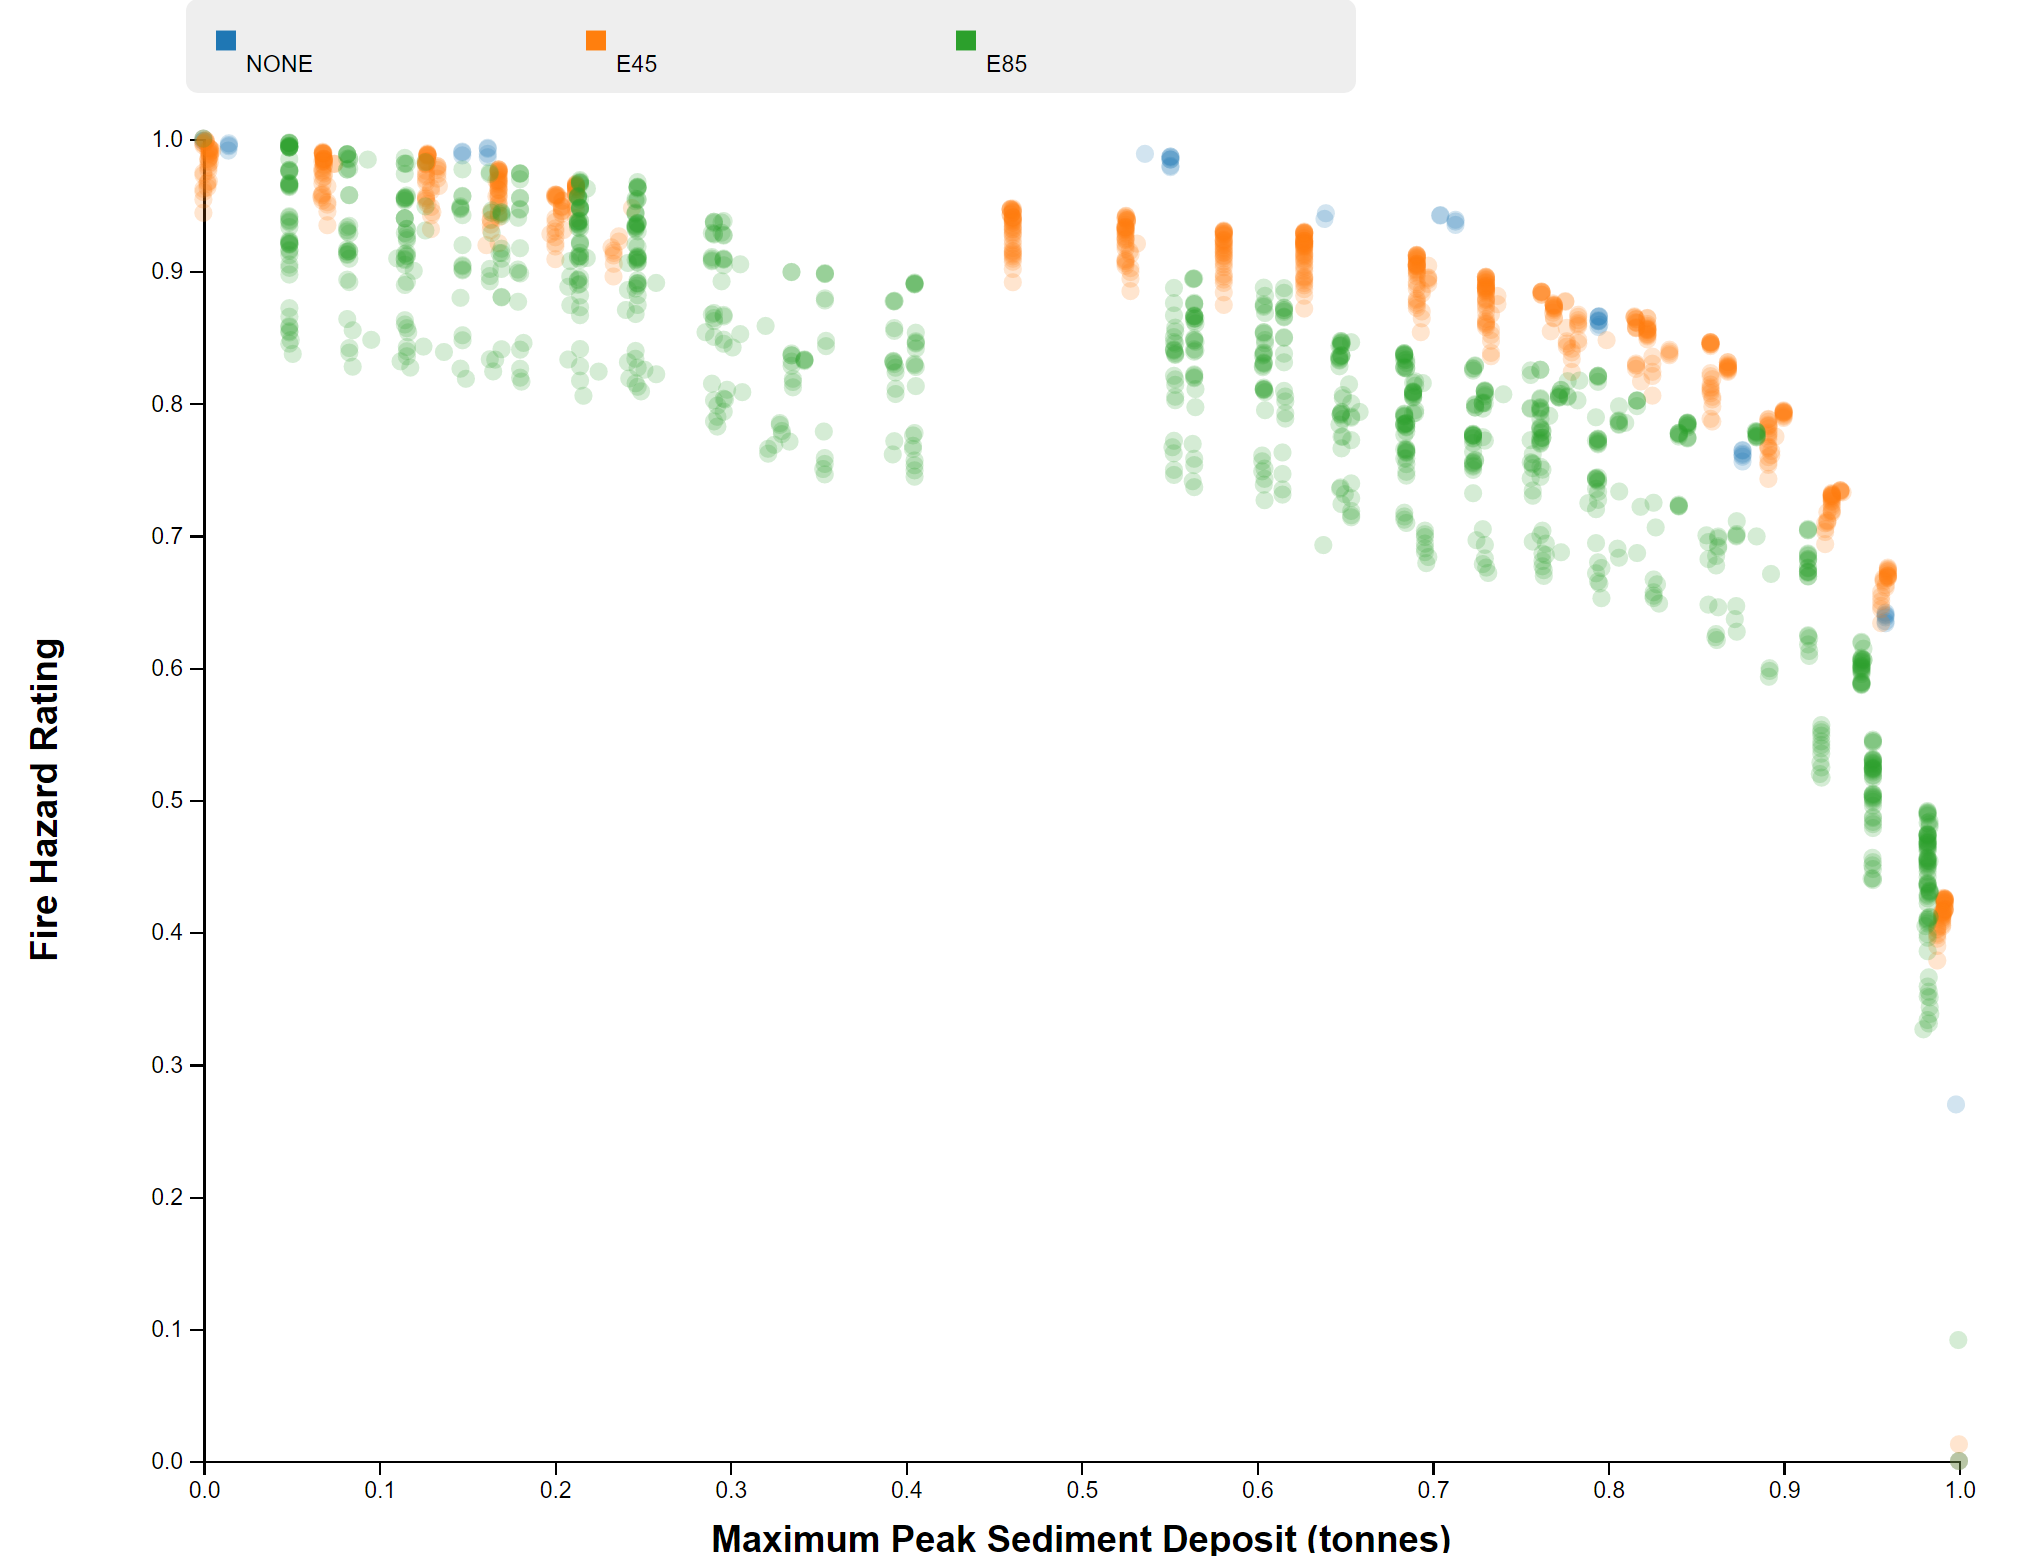
\includegraphics[width=.75\textwidth]{../images/2DSlice_Sed_Fire}
\caption[Sediment delivery vs. fire hazard for all climate scenarios]{Sediment delivery versus fire hazard for all climate scenarios.}
\label{fig:pairplotSedFire}
\end{figure}

\begin{table}[]
\centering
\caption[Sediment delivery-fire hazard conflict across climate scenarios]{Conflict between sediment delivery and fire hazard across climate scenarios.}
\label{tab:pairConflict-SedFire}
\begin{tabular}{llll}
\textbf{}     & \textbf{$C_{ij}$} & \textbf{$c_{ij,\rho}$} & \textbf{$c_{ij,d}$} \\ \hline
\textbf{None} & 0.36039           & 0.9927                 & 0.3630              \\
\textbf{E45}  & 0.36097           & 0.9853                 & 0.3664              \\
\textbf{E85}  & 0.38261           & 0.9514                 & 0.4021
\end{tabular}
\end{table}

\subsection{Discussion}
We divide our discussion of results into three sections: first, the decreasing provision of individual ecosystem services with climate change; second, the increase in the number of solutions and in the range of NSO habitat available; and third, conflict and the joint provision of ecosystem services.

\subsubsection{Decreasing provision of individual ecosystem services}
We observe decreasing provision of individual ecosystem services with increasing severity of climate change. In particular, we see that the difference between no climate change (None) and mild climate change (E45) was greater than the difference between mild climate change (E45) and severe climate change (E85). Refer to Table \ref{tab:frontiersSummary}. This suggests that, at least for the ecosystem services in this study, the realization of climate change is more significant than the severity of that change.

\paragraph{Sediment delivery}
Investigating the cause of the degradation in objective provision, we find for sediment delivery that the average amount of sediment delivered per fuel removal increases with climate change. See Figure \ref{fig:avgSedimentDelivery}. The average sediment delivery per fuel removal under E45 is nearly twice the sediment delivery under the None scenario (81\% higher), and the E85 scenario is 0.4\% higher than that. This is driven by two underlying factors: the response in sediment delivery to prescribed burns and the frequency with which prescribed burns are assigned\footnote{For additional information on how stands are assigned a specific fuel removal technique such as thinning or prescribed burn, see the appendix, \S \ref{chap:appendix_drinkTreatments}.}. Our simulations show that increasing the severity of climate change causes pronounced increases in sediment delivery as a result of prescribed burns. We also find that relative to the None scenario, prescribed burns are assigned more frequently in the climate change scenarios -- 8 times more frequently in E45 and 10.1 times more frequently in E85. See Table \ref{tab:prscBurnsInClimChange}. These effects combine to produce the result seen in Figure \ref{fig:avgSedimentDelivery} of sediment delivery levels that increase with climate change severity.

\begin{figure}[ht]
\centering
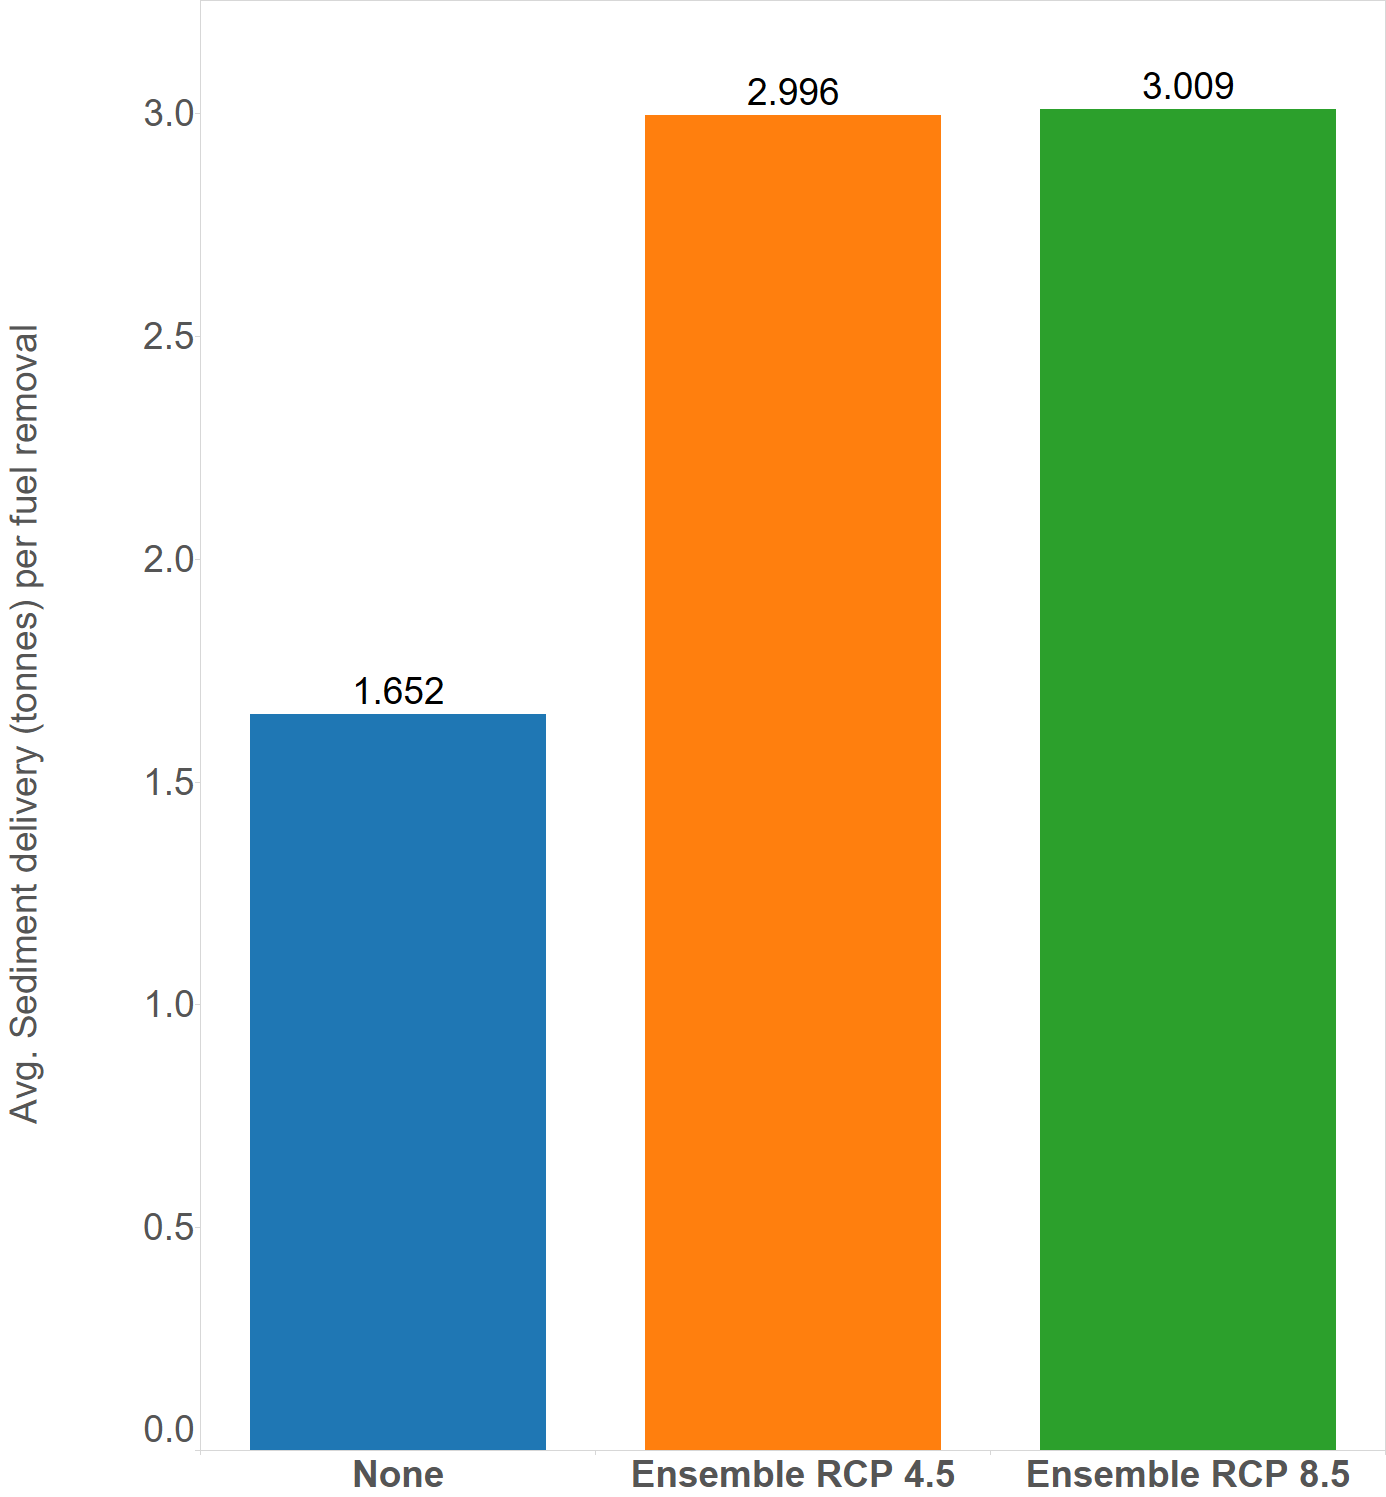
\includegraphics[width=.55\textwidth]{../images/AvgSedimentSpikes}
\caption[Average sediment delivery across climate scenarios]{Average spike in sediment delivery as a result of performing fuel removals for each climate change scenario.}
\label{fig:avgSedimentDelivery}
\end{figure}

\begin{table}[]
\centering
\caption[Frequency and impact of prescribed burns across climate scenarios]{Frequency and impact of prescribed burns for each climate scenario. The combination of more frequent prescribed burns and increased sediment delivery per prescribed burn results in the higher values of sediment delivery in E45 and E85 observed in Figure \ref{fig:avgSedimentDelivery}.}
\label{tab:prscBurnsInClimChange}
\begin{tabular}{llll}
                                                                                                           & \textbf{None} & \textbf{E45} & \textbf{E85} \\ \hline
\textbf{\begin{tabular}[c]{@{}l@{}}Average sediment delivery\\ (tonnes) from prescribed burn\end{tabular}} & 31.23            & 48.56          & 48.97          \\
\textbf{\begin{tabular}[c]{@{}l@{}}Number of prescribed\\ burns assigned\end{tabular}}                     & 34         & 272        & 344       
\end{tabular}
\end{table}

\paragraph{Fire hazard}
For the fire hazard objective, we first note that the increase in fire hazard with climate change severity is not simply due to the model selecting less area for treatment. This value is essentially constant across both treatment periods and all climate scenarios -- see Table \ref{tab:treatedAreas}. Instead, we find that the increase in fire hazard is due to the impact of climate change on the fuel model classification of the stands in the Drink Area. In E45 and E85, more stands are assigned a fuel model classification that is associated with higher fire hazard (refer to Table \ref{tab:firehazards} for the mapping from fuel models to fire hazard). This is shown in Figure \ref{fig:distOfFireHazards}, where we observe a larger percentage of stands having a fire hazard rating of either 4 or 5 under the E45 and E85 scenarios than in None.

\begin{table}[]
\centering
\caption[Area treated per period across climate scenarios]{Areas treated per period across climate scenarios. The values are nearly constant for both periods and for each climate scenario.}
\label{tab:treatedAreas}
\begin{tabular}{llll}
                                                                                                           & \textbf{None} & \textbf{E45} & \textbf{E85} \\ \hline
\textbf{Area treated (ha) in period 1} & 2427.31            & 2426.90 & 2414.58          \\
\textbf{Area treated (ha) in period 2}                     & 2427.56         & 2427.71        & 2427.63      
\end{tabular}
\end{table}

\begin{figure}[ht]
\centering
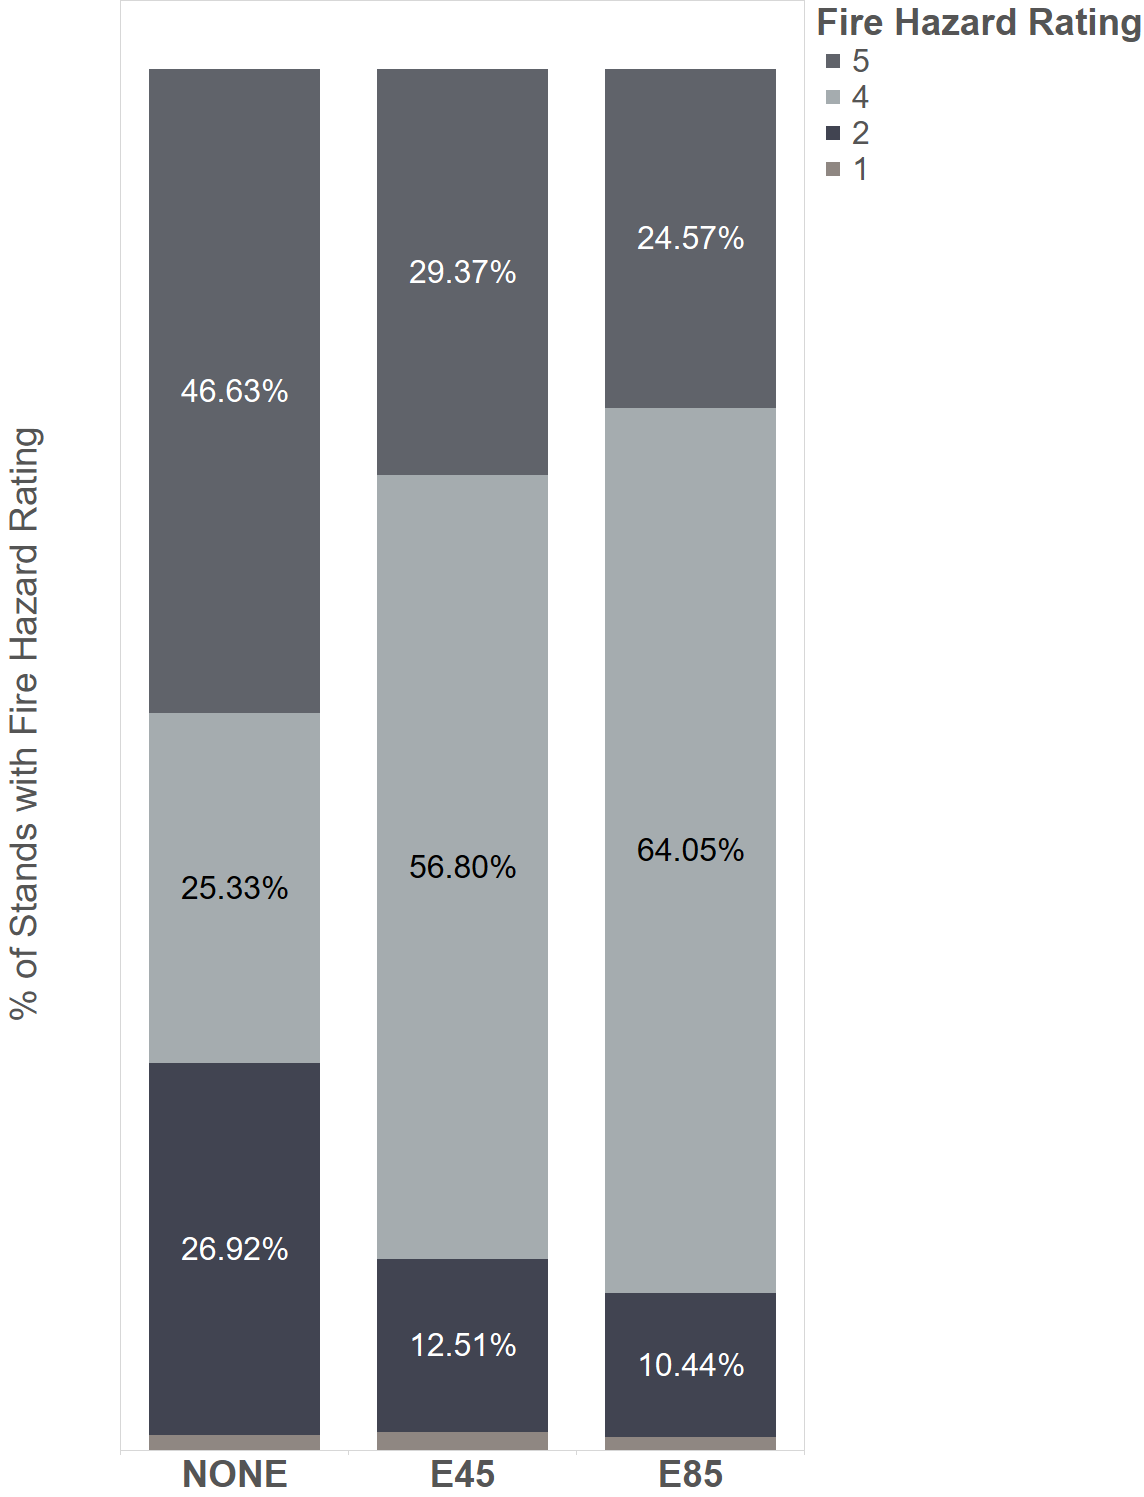
\includegraphics[width=.5\textwidth]{../images/FireHazardRatingsPerClimateScenario}
\caption[Distribution of fire hazard ratings over the Drink Area for each climate change scenario]{Distributions of fire hazard ratings across the Drink Area under each climate change scenario. Moving from left to right (in increasing climate change severity), we observe an increase in the percent of stands classified with more extreme fire hazards (ratings of 4 and 5).}
\label{fig:distOfFireHazards}
\end{figure}
% If we need a map, show a single map that shows the diff in FH at 2095 for a good sol from E85 - good sol from None

\paragraph{NSO habitat}
Lastly, we find that the decrease in NSO habitat is largely due to the effects of climate change on the vegetation in the Drink Area. Recall that of the criteria used to determine if a stand qualifies as NSO habitat, two of them are determined by vegetation characteristics: the presence of at least one tree with DBH $> 76$ cm and canopy closure of at least 60\%. While climate change has minimal impact on the former, the average canopy closure for stands in the Drink Area decreases with increasing severity of climate change. See Figure \ref{fig:canopyClosure}.

\begin{figure}[ht]
\centering
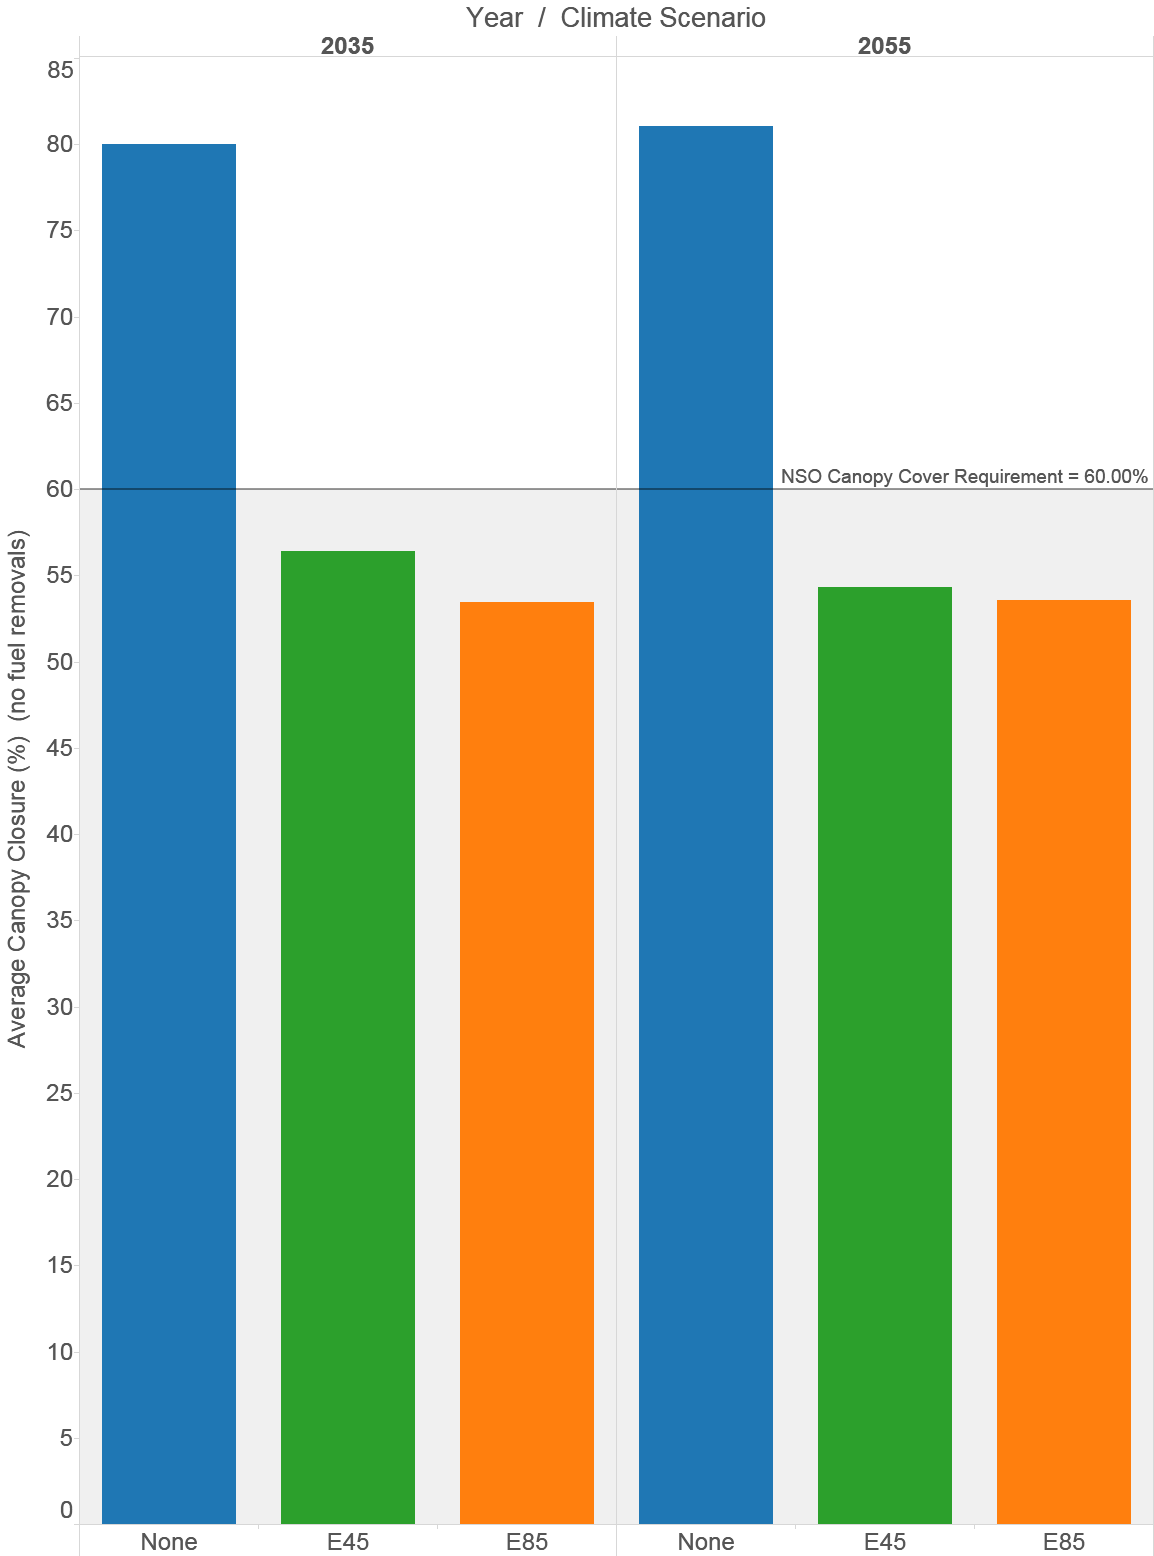
\includegraphics[width=.5\textwidth]{../images/AvgCanopyCover_NoTrtmts}
\caption[Average canopy closure in the Drink Area across climate scenarios]{Average canopy closure for stands in the Drink Area for each climate scenario. Shown are canopy closure values during years 2035 and 2055 (the years in which NSO habitat is measured) when no fuel removals are performed. We see that with increasing climate change severity, canopy closure decreases.}
\label{fig:canopyClosure}
\end{figure}


\subsubsection{Variation in number of solutions and range of values for NSO habitat}
With increasing climate change severity, we noted an increase in the number of solutions generated by our model:  51 for $Z_{\text{None}}$, 701 for $Z_{\text{E45}}$, and 1083 for $Z_{\text{E85}}$. We speculate that the cause of this is the same as that of the increase in the range of NSO habitat provided -- the impact of fuel removals on whether a stand qualifies as NSO habitat.

We see in Table \ref{tab:nsoHabDQs} the number of instances in which performing a fuel removal disqualifies a stand from being NSO habitat. Let us refer to such a fuel removal as a ``disqualifying treatment.'' We notice that disqualifying treatments occur more than twice as frequently in E45 and E85 than in None. To understand why the increase in the number of disqualifying treatments increases the number of solutions, consider a stand $i$ which is suitable NSO habitat under all fuel removal schedules $r$ in the None scenario. Then the values of sediment delivery and fire hazard would vary with selection of $r$, but the resulting NSO habitat would always be the same. Now, in the case of climate change (say E45) some fuel removal schedules $r$ are disqualifying treatments. That is, the selection of $r$ also now changes whether stand $i$ qualifies as NSO habitat. This influences the objective function value via equation \eqref{eqn:constraintDefOwl}, and it also affects the clustering associated with that stand (constraints \eqref{eqn:constraintClusterTriggers} and \eqref{eqn:constraintPVarTriggers}). This leads to solutions that did not exist in None.

\begin{table}[ht]
\centering
\caption[Frequency of NSO habitat disqualifications across climate scenarios]{Shown here are the number of times for each climate scenario that a fuel removal triggers the disqualification of a stand from being NSO habitat.}
\label{tab:nsoHabDQs}
\begin{tabular}{ll}
\textbf{Climate change scenario} & \begin{tabular}{@{}l@{}}\textbf{Disqualifications of NSO habitat} \\ \textbf{as a result of fuel removals}\end{tabular} \\ \hline
\textbf{None}                    & 24                                                                               \\
\textbf{Ensemble RCP 4.5}        & 63                                                                               \\
\textbf{Ensemble RCP 8.5}        & 67                                                                              
\end{tabular}
\end{table}

If the disqualifying treatments generated little fire hazard reduction in return for the disqualification of NSO habitat, then these decisions would not be part of the optimal solutions $\mathbf{x} \in P$. However, we also find that the reduction in fire hazard for a given disqualifying treatment increases with climate severity (Figure \ref{fig:nsoHabDQFHEfficacy}). This leads to greater incentive for the model to sacrifice NSO habitat in favor of fire hazard reduction.

\begin{figure}[ht]
\centering
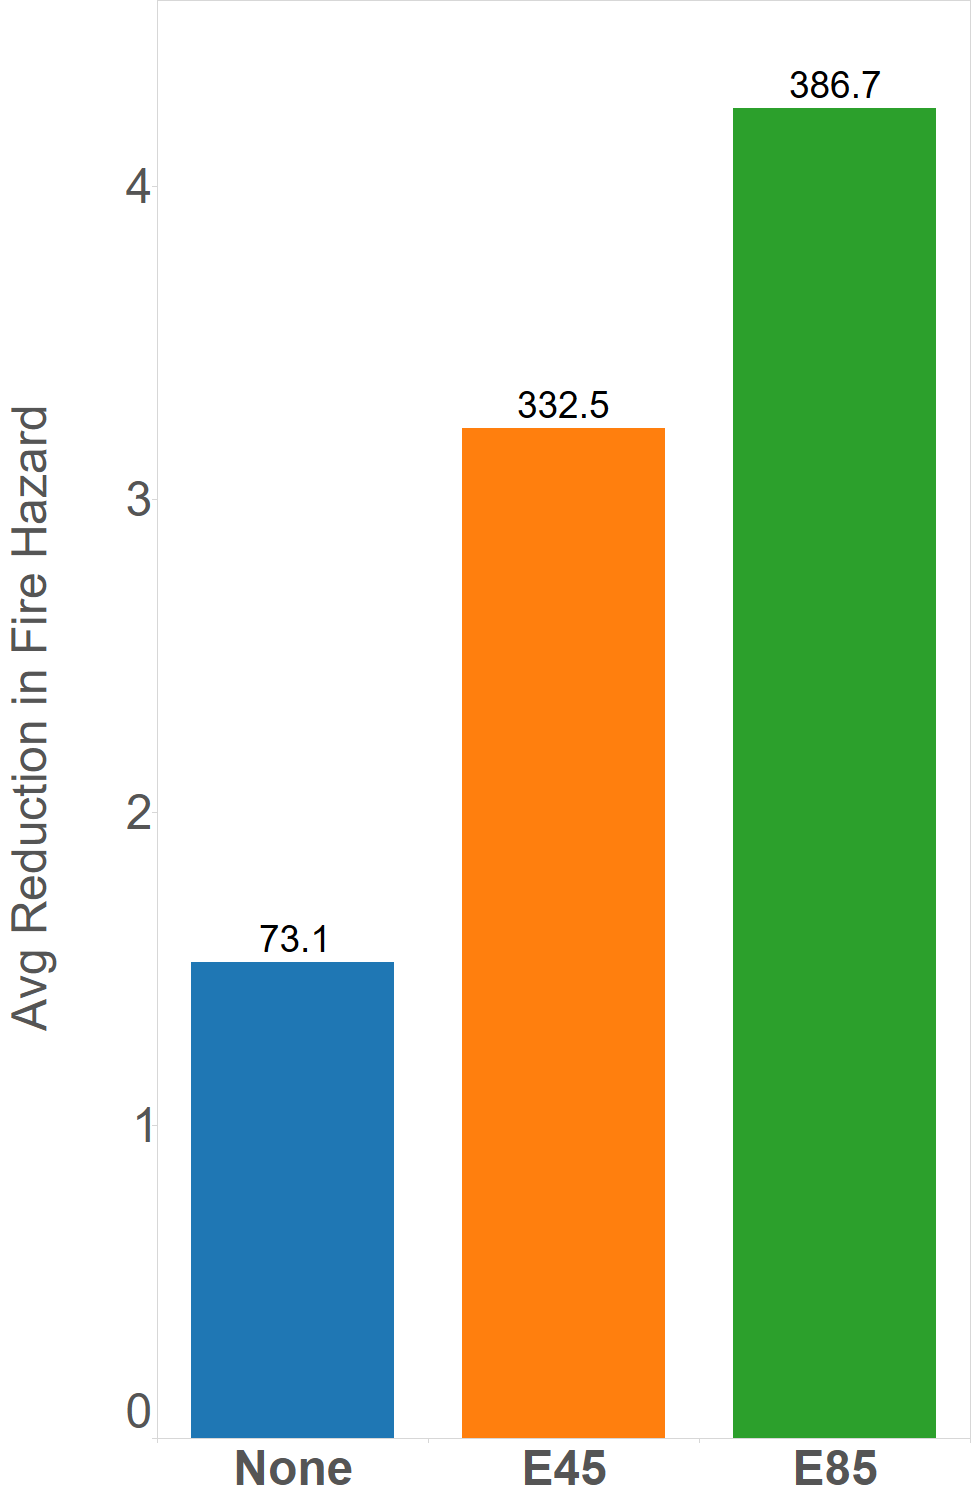
\includegraphics[width=.5\textwidth]{../images/AvgFireHazardEffectivenessForNSODQs}
\caption[Efficacy of fuel removals for NSO habitat disqualification]{Some stands may always be NSO habitat and others may never be NSO habitat, regardless of model decisions. For those stands which vary based on model decisions, we see here the average efficacy of fuel removals which disqualify their being NSO habitat. This value increases with increasing climate change, indicating greater incentive for the model to forgo NSO habitat in favor of fire hazard reduction.}
\label{fig:nsoHabDQFHEfficacy}
\end{figure}

Together, these factors lead to an increase in the number of solutions as well as greater diversity in the total amount of NSO habitat provided by the models.

%Could add a figure to show the map of what's NSO hab in a good sol vs a bad sol. Already made this on my work computer. Use it if req'd

\subsubsection{Conflict and the joint provision of ecosystem services}
We observe a decreasing hypervolume with increasing climate change severity. Lower values for the hypervolume are indicative of more conflict, meaning that climate change induces more conflict among the ecosystem services and leads to less joint provision of objectives.

The difference in hypervolume between None and E45 $I_{H1}(Z_\text{None}) - I_{H1}(Z_\text{E45}) \approx 0.01$. Recall that a difference of $h$ in hypervolumes equates to a difference of $h^{1/M}$ in each objective (Figure \ref{fig:Hypervol10percent}). Thus, despite the small size of the difference between $I_{H1}(Z_\text{None})$ and $I_{H1}(Z_\text{E45})$, it signifies an additional joint provision of objectives of approximately 21.6\%. This difference is greater between None and E85, approximately 0.05, representing an additional joint provision of ecosystem services of approximately 36.2\%.

From the hypervolumes alone, it is uncertain whether None represents a strictly better frontier than either E45 or E85 or if, despite their smaller hypervolume values, E45 and E85 enclose some region of the objective space that is not enclosed by None. Any such region would extend further into the objective space, representing the presence of solutions that achieve greater joint provision of ecosystem services. The results of the binary hypervolume were presented in Table \ref{tab:binaryHypervols}.

The results show that no frontier is dominated by any other, and each frontier encloses some region of the objective space not enclosed by the others. For the pairs of frontiers for which the binary hypervolume is greatest ($(Z_\text{None},Z_\text{E85})$ and $(Z_\text{E45},Z_\text{E85})$), this additional extension into the objective space is most obvious in Figure \ref{fig:pairplotSedFire}. We see for values of sediment delivery between 0.15 and 0.8 that None appears to dominate E45 which appears to dominate E85. Further, for sediment delivery values between 0.8 and 1, it appears that E45 dominates E85 and None, between which any domination relationship is difficult to discern.

The existence of these areas leads to the lower value of conflict $C_{ij}$ between sediment delivery and fire hazard in None and E45 than in E85. We note the success of the conflict metric $C_{ij}$ here: all frontiers in the sediment delivery-fire hazard plane of Figure \ref{fig:pairplotSedFire} are similar. They have similar shape and achievement towards the sub-dimensional ideal solution, yet the metric is able to distinguish differences in conflict between them.

For the other pairwise objective comparisons, as we saw in Figures \ref{fig:pairplotNSOSed} and \ref{fig:pairplotNSOFire}, the distribution of solutions more closely resembles a uniform two-dimensional scattering. There is no clear conflict pattern between them like that which we saw in Figure \ref{fig:pairplotSedFire}. As a result, $C_{ij}$ reports little conflict between these objective pairs, as desired. However it varied in unexpected ways between the climate scenarios. In these cases, we find that the distance component $c_{ij,d}$ was primarily responsible for the variations, as the rank correlations tended to be insignificantly different from 0.5. It appears the conflict metric $C_{ij}$ is susceptible to such variations when neither the $c_{ij,d}$ nor $c_{ij,\rho}$ component tends towards their limiting values of 0 and 1.

% In general, however, it was really awesome.
However, in general, we find our process of utilizing the hypervolume measures and the proposed conflict metric to have been successful in quantifying conflict within and among the frontiers. The pairwise conflict metric successfully identified the pair of objectives which demonstrated the most conflict, and the hypervolumes indicated which climate scenarios allow for greater joint provision of ecosystem services.
\chapter{Case Study: Impacts of climate change on competing forest ecosystem services}
\label{ch:caseStudyDeschutes}
To demonstrate the application of the hypervolume indicators and the proposed pairwise objective metric to the analysis of conflict in multi-objective systems, we perform a case study on forest management in the Deschutes National Forest. We compare the conflict among ecosystem services in three multi-objective systems: one in which climate change is ignored, one in which climate change is predicted to be mild, and one in which it is predicted to be severe. For each climate change scenario, we solve a multi-objective mathematical program that optimizes ecosystem service achievement. The model aims to minimize fire hazard and sediment delivery while maximizing habitat for the northern spotted owl. In the coming sections we describe the study area and the importance of each of these ecosystem services. We then formally define the mathematical program solved for each climate change scenario, describe the climate scenarios considered, and finally present and discuss the results.

\section{Study area and selection of ecosystem services}
\label{sec:studyArea}
%To provide context for the selection of ecosystem services for the model, we first describe the area in which the case study was conducted.
Our study area is the Drink Planning Area. It consists of 7056 ha of federally owned forest land on the east slopes of the Cascade Mountain Range located within the Deschutes National Forest. See Figure \ref{fig:drinkOverview}. Having never undergone logging or treatment, the Drink contains large areas of old growth forest. The large swaths of old growth forest in the Drink make it prime habitat for the northern spotted owl (NSO) (\textit{Strix occidentalis caurina}, Figure \ref{fig:nso}), an iconic % (albeit controversial \cite{simberloff1998flagships}) 
inhabitant of Pacific Northwest forests that is listed as a federally threatened species \cite{congress1973endangered}. However, the same old growth conditions that render the area suitable habitat for the NSO also render it susceptible to high-severity wildfires. Such a wildfire would put at risk the NSO's habitat \cite{courtney2004scientific} as well as one of the Drink's other notable features - the municipal watershed for the cities of Bend, OR and Sisters, OR. Wildfires pose a threat to these cities' water supply, because they can cause soil water repellency, surface runoff, and debris torrents \cite{ice2004effects} which degrade watershed quality.

\begin{figure}[ht]
\centering
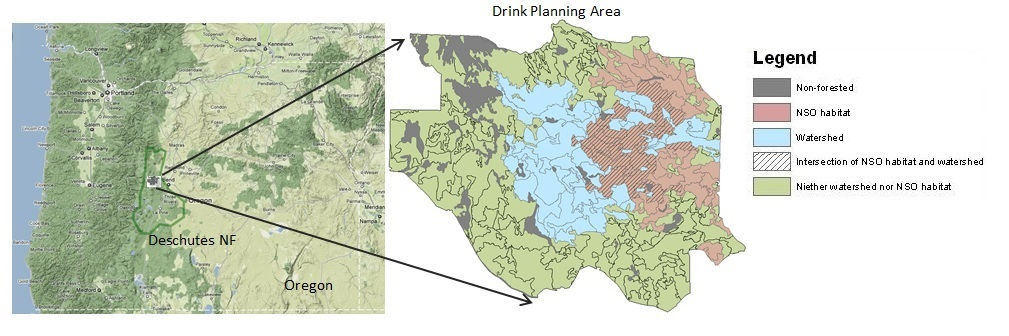
\includegraphics[width=.9\textwidth]{../images/Drink_Overview}
\caption[Overview of the study system, the Drink Planning Area]{Overview of the study system, the Drink Planning Area, consisting of 7056 ha in the Deschutes National Forest. The Drink Area contains old growth forest that make it suitable habitat for the northern spotted owl. It also houses the municipal watershed for Bend, OR and Sisters, OR.}
\label{fig:drinkOverview}
\end{figure}

\begin{figure}
\centering
\caption[Northern spotted owl]{The northern spotted owl is a threatened species whose habitat includes forests in the Pacific Northwest, including the Drink Area.}
\label{fig:nso}
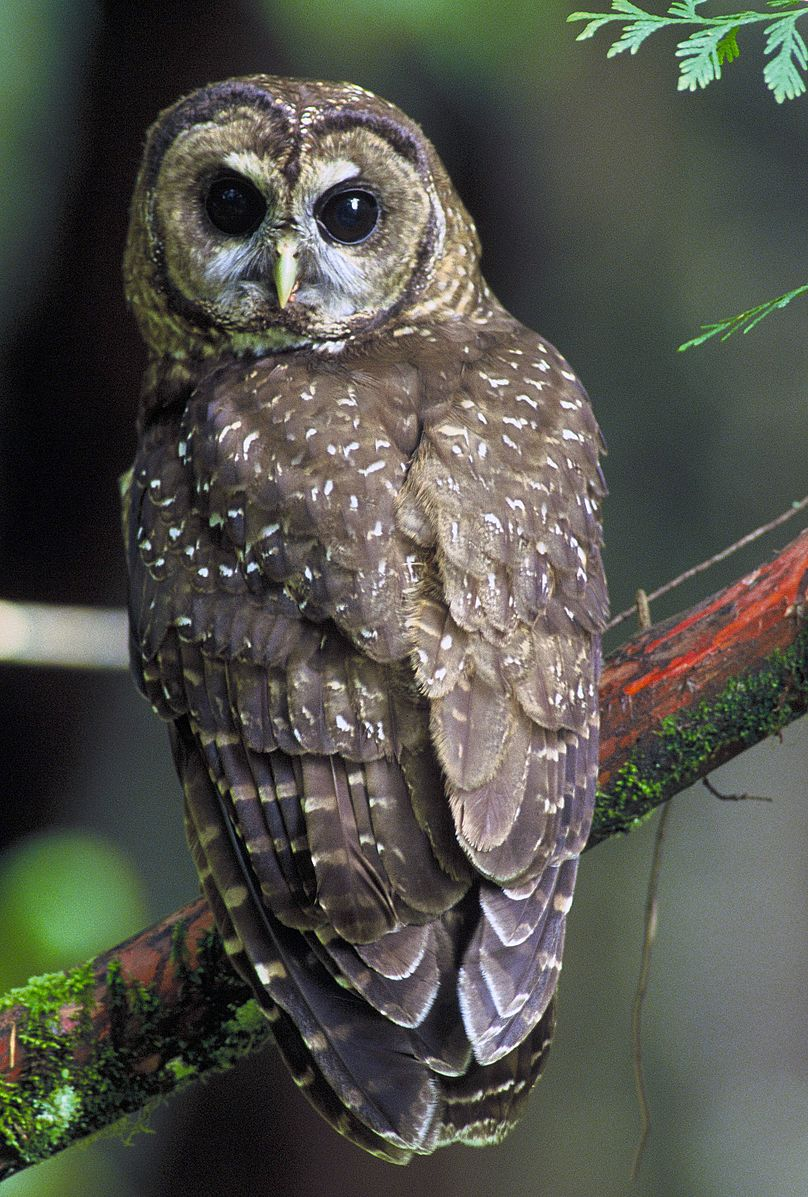
\includegraphics[width=.2\textwidth]{../images/NorthernSpottedOwl_USFWS}
\end{figure}

For these reasons, the managing entity, the United States Forest Service (USFS), would like to perform fuel removals in the Drink in order to reduce the area's fire hazard. However, performing these fuel removals has the potential to disrupt the habitat of the NSO \cite{bond2002short} and to induce short-term increases in sediment delivery \cite{o2005conceptual}. The latter is expected to be especially true in the Drink Area, where local USFS staff have noted that the watershed is unusually susceptible to spikes in sediment delivery as a result of foot traffic and other activities that occur within the watershed.

We developed a multi-objective mathematical program that optimizes the joint provision of these conflicting ecosystem services\footnote{These represent only a subset of the ecosystem services of concern to the USFS in the Drink Area. While the USFS manages for many ecosystem services simultaneously, many of the services are stacked rather than bundled, meaning the ecosystem services are not in conflict. These services need not all be considered in the multi-objective model, because the selection and maximization of one ecosystem service entails the maximization of all in the stack. For this reason, we have disregarded non-conflicting ecosystem services and selected a minimal bundle on which to employ multi-objective optimization. Those that do not conflict can be stacked post-optimization.}.

\section{The multi-objective model}
The multi-objective model is a zero-one mathematical program that assigns spatiotemporal prescriptions for fuel removals across the Drink Area to optimize the joint provision of ecosystem services. Spatially, the model prescribes fuel removals across 303 forest treatment units into which the Drink has been divided (the interior polygons in Figure \ref{fig:drinkOverview}). Temporally, the model operates over an 80-year planning horizon, from 2015 to 2095. The fuel removals are scheduled in two 20-year treatment periods: 2015-2035 and 2035-2055. For each treatment unit, the model may prescribe fuel removals in the first period, the second period, neither, or both.

To ensure long-term efficacy of the fuel removals, the model minimizes the fire hazard rating of the Drink Area at the end of the 80-year planning horizon. To mitigate impacts of the fuel removals on NSO habitat, the model maximizes the area of NSO habitat at the end of each planning period. Similarly, the model minimizes the short-term spikes in sediment delivery resulting from the application of fuel removals, which are assumed to be performed at the midpoint year in the treatment periods (years 2025 and 2045). Note that because a wildfire is expected to severely degrade NSO habitat and cause a mass delivery of sediment, we assume that the long-term minimization of fire hazard serves as a proxy for both the long-term protection against a mass sediment delivery event and for the protection of habitat for the northern spotted owl.

Figure \ref{fig:drinkPlanningHorizon} contains a schematic of the planning horizon which shows the timing of these events.

\begin{figure}
\centering
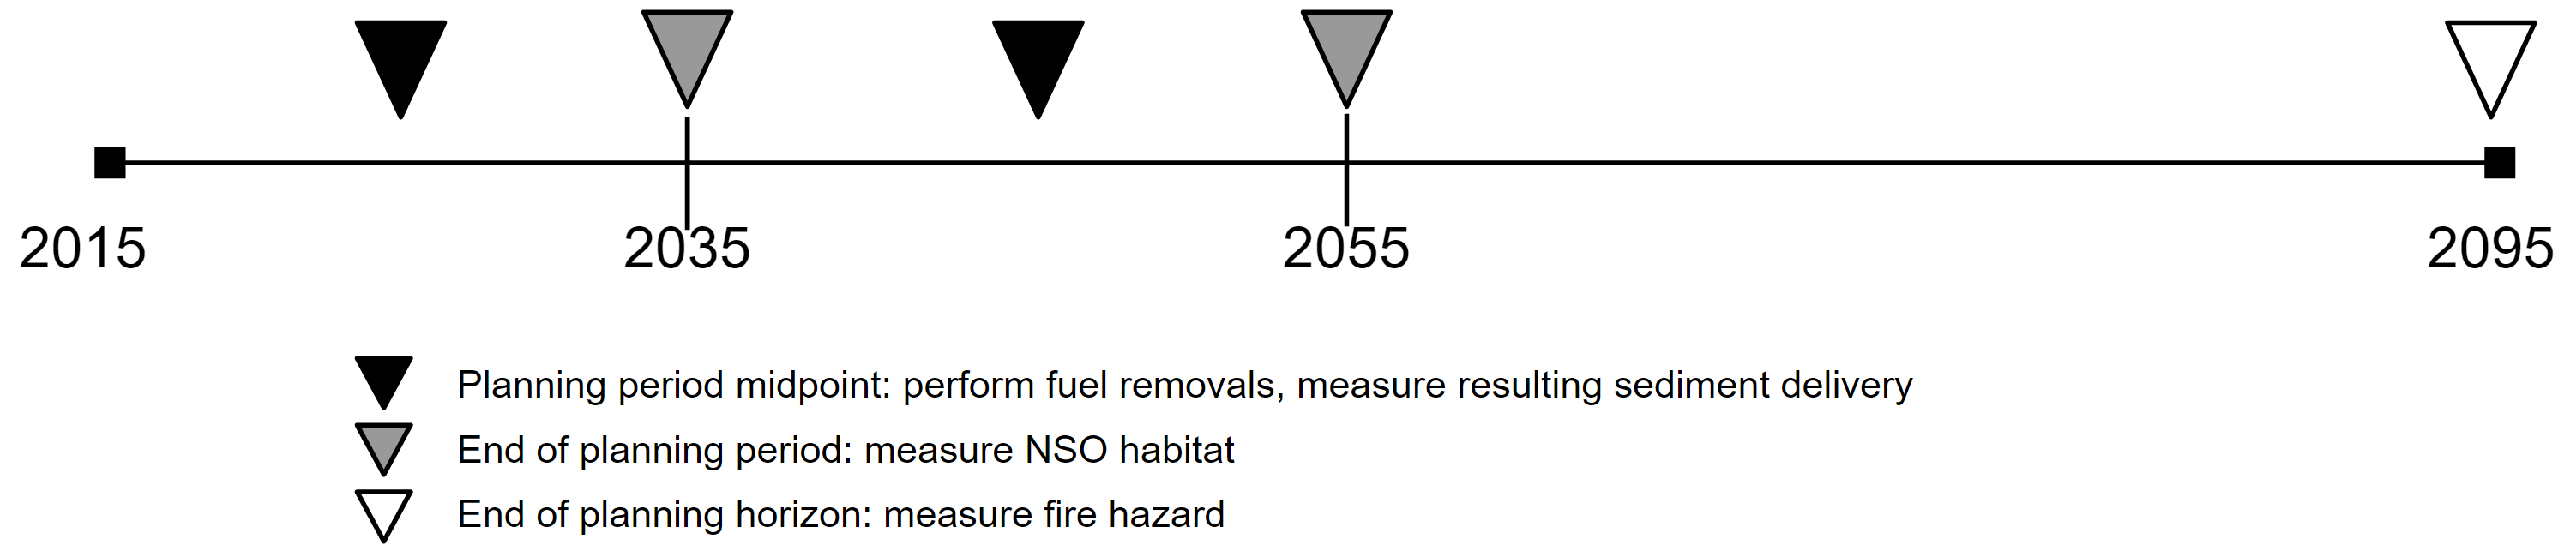
\includegraphics[width=.9\textwidth]{../images/Drink_PlanningHorizon_Sketch}
\caption[Planning horizon for the case study]{The planning horizon used in the case study spans the 80 year period from 2015 to 2095. Fuel removals may be performed in the first period (2015-2035), the second period (2035-2055), both, or neither. Fuel removals are assumed to be performed at the mid-point years of each period (black triangles). Sediment delivery is measured on treatment years. Treatment units' suitability for NSO habitat is measured at the end of the planning periods (gray triangles), and treatment units' fire hazard ratings are measured at the end of the planning horizon (white triangle).}
\label{fig:drinkPlanningHorizon}
\end{figure}

\subsection{Notation}
\label{subsec:notation}
We use the following notation in the development of the model:

\paragraph{Model parameters}
\begin{itemize}
\item \textbf{$i \in I$:} the set of treatment units comprising the Drink Area ($|I| = 303$)

\item \textbf{$a_i$:} the area of treatment unit $i$

\item \textbf{$r \in R$:} the set of fuel removal prescriptions:
	$$
	r =
	\begin{cases}
	1 &\text{ fuel removals in the first period (2015-2035)}\\
	2 &\text{ fuel removals in the second period (2035-2055)}\\
	3 &\text{ fuel removals in both periods}\\
	0 &\text{ no fuel removals performed in either period}
	\end{cases}
	$$
	
\item \textbf{$F_{i,r}$:} the area-weighted fire hazard rating of treatment unit $i$ at the end of the planning horizon if prescribed to fuel removal schedule $r$. For instance, if a treatment unit $i$ under fuel removal schedule $r$ has a fire hazard rating of 4 in the year 2095, and its area is 10 hectares, then $F_{i,r} = 40$. The metric for fire hazard rating used in this analysis was developed by Schroder \textit{et al.} \cite{schroder2016multi} specifically for the Drink Area. It uses fire characteristics from the set of fuel models proposed by Anderson \cite{anderson1982aids} in order to assign a fire hazard rating. We expand the rating system to include fuel models not present in Schroder \textit{et al.} See Table \ref{tab:firehazards} for the mapping of fuel models to fire hazard ratings.

The USFS's Climate-Forest Vegetation Simulator (Climate-FVS) was used to generate the fuels and vegetation characteristics of the treatment units in order to determine their fire hazard rating. Initial vegetation data for Climate-FVS came from the 2012 GNN structure map (\url{http://lemma.forestry.oregonstate.edu/data/structure-maps}) from Oregon State University's Landscape Ecology, Modeling, Mapping \& Analysis (LEMMA) group. Plots from the LEMMA database were mapped to the treatment units in the Drink area in order to produce tree and treatment unit lists. These lists were used with Climate-FVS to simulate the treatment units' vegetation and fuels characteristics forward for the duration of the planning horizon under each climate scenario. Input climate data for Climate-FVS was obtained through the Climate-FVS climate data server \cite{climateFVSReadyData}.

\begin{table}[!ht]
\centering
\resizebox{\textwidth}{!}{%
\begin{tabular}{lccrrr}
\multicolumn{1}{c}{Fuel Model} & \multicolumn{1}{c}{\textbf{Fire Hazard Rating}} & \multicolumn{1}{c}{Group} & \multicolumn{1}{c}{Flame length (m)} & \multicolumn{1}{c}{Rate of spread (m/hr)} & \multicolumn{1}{c}{Total fuel load (tons/ha)} \\ \hline
4*                              & \textbf{5}                                       & Shrub                     & 5.79                                 & 1508.76                                   & 32.12                                         \\
5                               & \textbf{4}                                       & Shrub                     & 1.22                                 & 362.10                                    & 8.65                                          \\
8                               & \textbf{1}                                       & Timber                    & 0.30                                 & 32.19                                     & 12.36                                         \\
9*                              & \textbf{2}                                       & Timber                    & 0.79                                 & 150.88                                    & 8.65                                          \\
10                              & \textbf{2}                                       & Timber                    & 1.46                                 & 158.92                                    & 29.65                                         \\
11*                             & \textbf{2}                                       & Logging Slash             & 1.07                                 & 120.7                                     & 28.42                                         \\
12                              & \textbf{4}                                       & Logging Slash             & 2.44                                 & 261.52                                    & 85.50                                         \\
13                              & \textbf{5}                                       & Logging Slash             & 3.20                                 & 271.58                                    & 143.57                                       
\end{tabular}%
}
\caption[Fire hazard ratings used in multi-objective model]{Fire hazard rating system used here, originally employed by Schroder \textit{et al.} \cite{schroder2016multi}. Non-forested areas are assigned a fire hazard value of 0.\\
Asterisks (*) denote fuel models not present in Schroder \textit{et al.}\\
The fuel model column refers to the Anderson fuel model ratings \cite{anderson1982aids}.}
\label{tab:firehazards}
\end{table}

\item \textbf{$I_{\omega,t}$:} the set of treatment units that qualify as NSO habitat at the end of planning period $t$ under at least one fuel removal schedule. The treatment units that qualify as NSO habitat at the end of a planning period $t$ are those that meet the following three criteria in year $t$, as specified by the USFS:
	\begin{enumerate}
	\item elevation less than 1830 m
	\item the presence of trees with diameter at breast height (DBH) at least 76 cm
	\item canopy closure of at least 60\%
	\end{enumerate}
The elevation requirement was checked using a digital elevation model from the US Department of Agriculture's GeoSpatial Data Gateway; canopy closure and large tree criteria were determined using the simulated vegetation characteristics output from Climate-FVS.

In addition, to account for the large habitat requirements of the NSO, treatment units must be members of a cluster exceeding 200 ha in size, the entirety of which meets the aforementioned NSO habitat criteria. Treatment units that meet the first three criteria but are not part of such a cluster are less valuable NSO habitat and therefore have their contributions to the total owl habitat discounted by a factor of $e$.

\item \textbf{$e$:} the discount factor applied to NSO habitat when it is not part of a contiguous habitat cluster at least 200 ha in size. Following the convention used in Schroder \textit{et al.} \cite{schroder2016multi}, we set $e = 0.5$.

\item \textbf{$j \in R_{i,t}$:} the set of fuel removal schedules such that treatment unit $i$ qualifies as NSO habitat at the end of planning period $t$. For instance, consider treatment unit $i=15$ and planning period $t=2$ (2035-2055). We seek to find the set of fuel removal prescriptions $r \in R$ such that treatment unit 15 is suitable NSO habitat at the end of planning period 2 (in year 2055). We enumerate the vegetation characteristics of treatment unit 15 for all possible fuel removal schedules and determine that if fuel removals are assigned in the second planning period, then treatment unit 15 does not qualify as NSO habitat in year 2055. Thus, $R_{15,2} = \{0,1\}$, since for $r=0$ (no fuel removals performed) and $r=1$ (fuel removals performed in first period only), treatment unit 15 does qualify as NSO habitat in 2055.

\item \textbf{$s_{i,t}$:} the amount of sediment (in tonnes) delivered to the watershed as a result of performing fuel removals on treatment unit $i$ in planning period $t$. The contributions of sediment delivery from treatment of treatment unit $i$ in period $t$ were determined using the online GIS tool for the Watershed Erosion Prediction Project (WEPP) \cite{frankenberger2011development}. WEPP GIS was selected for use, because it is able to take climate variables into account. The climate variables used in our simulations are the same custom climate data described above for use with Climate-FVS, obtained through the Climate-FVS data server.

WEPP GIS also takes soil textures, treatment types, and duration of simulation as inputs. Soil texture data for the Drink area was obtained from the USDA's Soil Survey Geographic (SSURGO) database, treatment types are those specified in \S \ref{chap:appendix_drinkTreatments}, and the years of simulation correspond to the treatment years in the planning horizon (2015-2095).

\item \textbf{$c \in C$:} Recall that the quantification of NSO habitat depends on the availability of large contiguous habitat patches; areas of NSO habitat less than than 200 ha in size are discounted. In order to determine when habitat is provided in sufficiently large areas, we must enumerate the set of clusters of treatment units whose combined area exceeds 200 ha. This set of clusters is the set $C$.

\item \textbf{$i \in D_c$:} Given a cluster $c \in C$, the set $D_c$ is the set of treatment units that comprise cluster $c$.

\item \textbf{$c \in C_i$:} Given a treatment unit $i$, we define the set $C_i$ as the set of clusters that contain treatment unit $i$

\item \textbf{$A$:} the maximum area in hectares that may be treated in either planning period. We constrain the allowable treatment area per period to account for the limited availability of work crews to perform the fuel removals. Following guidance from the USFS, we set $A = 2428$ ha (approximately 6000 ac).

\item \textbf{$\ell$, $u$:} the lower and upper bounds, respectively, on the relative fluctuation in the area treated in periods 1 and 2. These bounds are used to enforce regulation in the workflow for the USFS. Here we use values such that the area for which fuel removals are performed does not fluctuate more than 20\% between treatment periods; that is, we set the lower bound $\ell = 0.8$ and the upper bound $u = 1.2$.
\end{itemize}

\paragraph{Decision Variables}
$$
x_{i,r} = \begin{cases}
1 &\text{ if treatment unit $i$ is prescribed to treatment schedule $r$}\\
0 &\text{ otherwise}
\end{cases}
$$ 

\paragraph{Indicator Variables}
\begin{itemize}
\item \textbf{$q_{c,t} = 1$} if all treatment units in cluster $c$ qualify as NSO habitat at the end of planning period $t$; $q_{c,t} = 0$ otherwise
\item \textbf{$p_{i,t} = 1$} if in planning period $t$ treatment unit $i$ is part of a cluster $c$ such that $q_{c,t} = 1$; $p_{i,t} = 0$ otherwise
\end{itemize}

\paragraph{Accounting Variables}
\begin{itemize}
\item \textbf{$S_t$:} the total sediment delivered to the watershed from performing fuel treatments in planning period $t$
\item \textbf{$O_t$:} the amount of NSO habitat (in hectares) at the end of planning period $t$
\item \textbf{$H_t$:} the total area (in hectares) treated in planning period $t$
\end{itemize}

\subsection{Model formulation}
The formulation of the multi-objective model is as follows:
\begin{align}
Minimize \quad & \notag\\
&\sum_{i\in I}\sum_{r\in R} F_{i,r} x_{i,r} \label{eqn:objFire} \\
&\max \{S_1,S_2\} \label{eqn:objSediment} \\
Maximize \quad & \notag\\
&\min \{O_1,O_2\} \label{eqn:objOwl}
\end{align}
Subject to:
\begin{align}
\sum_{i\in I_{\omega,t}} \left(a_i p_{i,t} + e a_i \left( \sum_{j \in R_{i,t}} x_{i,j}-p_{i,t} \right) \right) &= O_t \qquad \forall t \in \{1,2\} \label{eqn:constraintDefOwl}\\
\sum_{i\in I} \sum_{r\in 1,3} s_{i,1} x_{i,r} &= S_1 \label{eqn:constraintSediment1} \\
\sum_{i\in I} \sum_{r\in 2,3} s_{i,2} x_{i,r} &= S_2 \label{eqn:constraintSediment2} \\
\sum_{i \in D_c} \sum_{j \in R_{i,t}} x_{i,j} - |c| q_{c,t} &\ge 0 \qquad \forall t \in \{1,2\}, c \in C \label{eqn:constraintClusterTriggers} \\
\sum_{c \in C_i} q_{c,t} - p_{i,t} &\ge 0 \qquad \forall t \in \{1,2\}, i \in I_{\omega,t} \label{eqn:constraintPVarTriggers} \\
\sum_{r \in R} x_{i,r} &= 1  \qquad \forall i \in I \label{eqn:constraintOnePrescrip} \\
\sum_{i \in I} \sum_{r \in 1,3} a_i x_{i,r} &= H_1 \label{eqn:constraintAreaAcctg1} \\
\sum_{i \in I} \sum_{r \in 2,3} a_i x_{i,r} &= H_2 \label{eqn:constraintAreaAcctg2} \\
H_t &\le A \qquad \forall t \in \{1,2\} \label{eqn:constraintAreaRestr} \\
\ell H_1 - H_2 &\le 0 \label{eqn:constraintAreaFlucL} \\
-u H_1 + H_2 &\le 0 \label{eqn:constraintAreaFlucU} \\
x_{i,r}, p_i, q_c \in \{0,1\} \quad &\forall i \in I, r \in R, c \in C \label{eqn:constraintNonNeg}
\end{align}

Equations \eqref{eqn:objFire}-\eqref{eqn:objOwl} are the objective functions: equation \eqref{eqn:objFire} minimizes the cumulative fire hazard rating of the Drink Area at the end of the 80-year planning horizon, equation \eqref{eqn:objSediment} minimizes the maximum peak in sediment delivery for the two planning periods, and equation \eqref{eqn:objOwl} maximizes the minimum NSO habitat available at the end of the planning periods. Equation set \eqref{eqn:constraintDefOwl} defines the amount of NSO habitat available at the end of the planning horizons. Note that if treatment unit $i$ does not belong to a cluster of NSO habitat exceeding 200 hectares, then its area contribution to total NSO habitat is discounted by a factor of $e$. Equations \eqref{eqn:constraintSediment1} and \eqref{eqn:constraintSediment2} define the sediment delivered in planning periods one and two, respectively.

Inequality set \eqref{eqn:constraintClusterTriggers} controls the value of the cluster variables $q_{c,t}$ indicating clusters that meet the NSO habitat criteria in each of the planning periods. Inequality set \eqref{eqn:constraintPVarTriggers} controls the value of the $p_{i,t}$ variables indicating whether treatment unit $i$ is included in a cluster of NSO habitat at time $t$.

The set of equalities \eqref{eqn:constraintOnePrescrip} enforces the logical constraint that each treatment unit must be prescribed to exactly one fuel removal schedule. Equations \eqref{eqn:constraintAreaAcctg1} and \eqref{eqn:constraintAreaAcctg2} are accounting constraints for the total area treated in each planning period, and inequalities \eqref{eqn:constraintAreaRestr} ensure that this area does not exceed the predefined maximum. Inequalities \eqref{eqn:constraintAreaFlucL} and \eqref{eqn:constraintAreaFlucU} bound the fluctuation in treated area between the planning periods. Finally, constraint \eqref{eqn:constraintNonNeg} defines the decision and indicator variables as binary.

\section{Solution method}
We developed an implementation of T\'{o}th's Alpha-Delta algorithm \cite{TothThesis} to solve the model \eqref{eqn:objFire}-\eqref{eqn:constraintNonNeg} utilizing the IBM ILOG CPLEX optimization engine. For a problem with $M$ objectives, the Alpha-Delta algorithm finds the Pareto frontier by iteratively slicing the $M$-dimensional objective space with a tilted $M-1$-dimensional hyperplane. The algorithm was implemented using an alpha parameter of $\alpha = .01$ and delta parameters of $\delta_{Hab} = 1$ ha and $\delta_{Sed} = 2$ tonnes for the NSO habitat and sediment delivery objectives, respectively.

\section{Climate change scenarios}
\label{sec:climateChange}
Like other ecosystems, forests will undergo changes as a result of the changing climate. For instance, researchers anticipate new spatial distributions of tree species \cite{iverson1998predicting}, increased sediment delivery to streams \cite{Goode20121}, and increasing disturbance regimes such as wildfires, droughts, and insect infestations \cite{vose2012effects}. As these transformations occur, the ability of forests to provide ecosystem services will change.

The extent of change will likely depend on the severity of the realized climate change. Thus, to understand the potential impacts on ecosystem services, multiple climate change scenarios representing a range of severities should be considered. We use three in our case study: one scenario in which climate change is ignored, ``None''; one in which climate change is predicted to be mild, ``Ensemble RCP 4.5'' (also ``E45''); and one in which climate change is predicted to be severe, ``Ensemble RCP 8.5'' (also ``E85''). These scenarios differ in their assumption of the additional energy per unit area that will be absorbed by the atmosphere, a value known as radiative forcing (RF). E45 assumes an RF of 4.5 $W/m^2$ and E85 assumes 8.5 $W/m^2$. In general, larger values of RF correspond to more severe climate change.

A given value of radiative forcing does not map to a single prediction of climate change, because researchers may disagree in how the climate will respond to that amount of RF. This is why for a given RF numerous climate models exist. A common approach to handling the disagreement among the climate models is to use an ensemble of climate models that all assume the same RF. We adopt this approach here for our E45 and E85 scenarios.

Each of these scenarios corresponds to an ensemble of 17 climate models. These climate models originate from the Fifth Assessment (AR5) on climate performed by the Intergovernmental Panel on Climate Change (IPCC). The selection and assembly of the 17 climate models used in these ensembles was conducted by Cookston (2016) and the Climate-FVS team \cite{ClimateModelsInFVSEnsemble}.

The other scenario, None, ignores any effects of climate change. While the number of studies incorporating climate change is increasing, this is still a common assumption in modern studies such as Schroder \textit{et al}. (2013) \cite{schroder2016multi}. Because it has served as the basis for many past studies of ecosystem services, the None climate scenario serves as a control against which we will compare the other two.

Each climate scenario corresponds to a different parameterization of the model, since the vegetation, fuels, and sediment delivery data depend on climate. Thus, changing the climate scenario has the potential to affect the amount and location of NSO habitat, the effects of fuel removals on NSO habitat, the fire hazard of the Drink Area, the efficacy of the fuel removals in reducing fire hazard, and the sediment delivered as a result of fuel removals. This drives changes to the relationships among the ecosystem services as well, which we investigate using the aforementioned conflict measures.


\section{Results}
We parameterized and solved the multi-objective model (equations \eqref{eqn:objFire}-\eqref{eqn:constraintNonNeg}) for each of the climate scenarios, generating three efficient frontiers: $Z_{\text{None}}$, $Z_{E45}$, and $Z_{E85}$ for the None, Ensemble RCP 4.5, and Ensemble RCP 8.5 scenarios, respectively.  $Z_{\text{None}}$ consists of 51 solutions, $Z_{\text{E45}}$ consists of 701 solutions, and $Z_{\text{E85}}$ consists of 1083. Figure \ref{fig:frontiersAll} shows the frontiers in their 3-dimensional objective spaces, Figure \ref{fig:consolidatedFrontiers} shows all frontiers in a single 3-dimensional view, and Figure \ref{fig:frontiersPCPlot} provides a single parallel coordinates plot with all frontiers. The summary details of their objective achievements are listed in Table \ref{tab:frontiersSummary}.

\begin{table}[]
\centering
\caption[Summary of objective achievement across climate scenarios]{Summary of the performance of the efficient frontiers for each climate change scenario.}
\label{tab:frontiersSummary}
\begin{tabular}{lllll}
\multicolumn{2}{l}{}                                                  & \textbf{None} & \textbf{E45} & \textbf{E85} \\ \hline
\multirow{3}{*}{\begin{tabular}[c]{@{}l@{}}\textbf{Fire hazard (cumulative}\\ \textbf{area-weighted fire hazard)}\end{tabular}}       & \multicolumn{1}{l}{min} & 21,321.21      & 23,219.82     & 23,268.02     \\
                                            & \multicolumn{1}{l}{avg} & 21,406.26      & 23,324.41     & 23,369.57     \\
                                            & \multicolumn{1}{l}{max} & 21,933.29      & 23,973.79     & 23,724.98     \\ \hline
\multirow{3}{*}{\textbf{NSO habitat (ha)}}       & \multicolumn{1}{l}{min} & 2,532.33       & 2,412.18      & 2,171.10      \\
                                            & \multicolumn{1}{l}{avg} & 2,536.31       & 2,447.92      & 2,421.99      \\
                                            & \multicolumn{1}{l}{max} & 2,540.05       & 2,477.18      & 2,481.01      \\ \hline
\multirow{3}{*}{\textbf{Sediment delivery (tonnes)}} & \multicolumn{1}{l}{min} & 0             & 0            & 0            \\
                                            & \multicolumn{1}{l}{avg} & 10.25         & 27.98        & 31.19        \\
                                            & \multicolumn{1}{l}{max} & 24.57         & 63.43        & 69.68        
\end{tabular}
\end{table}


\begin{figure}[ht!]
  \subfloat[None]{%
    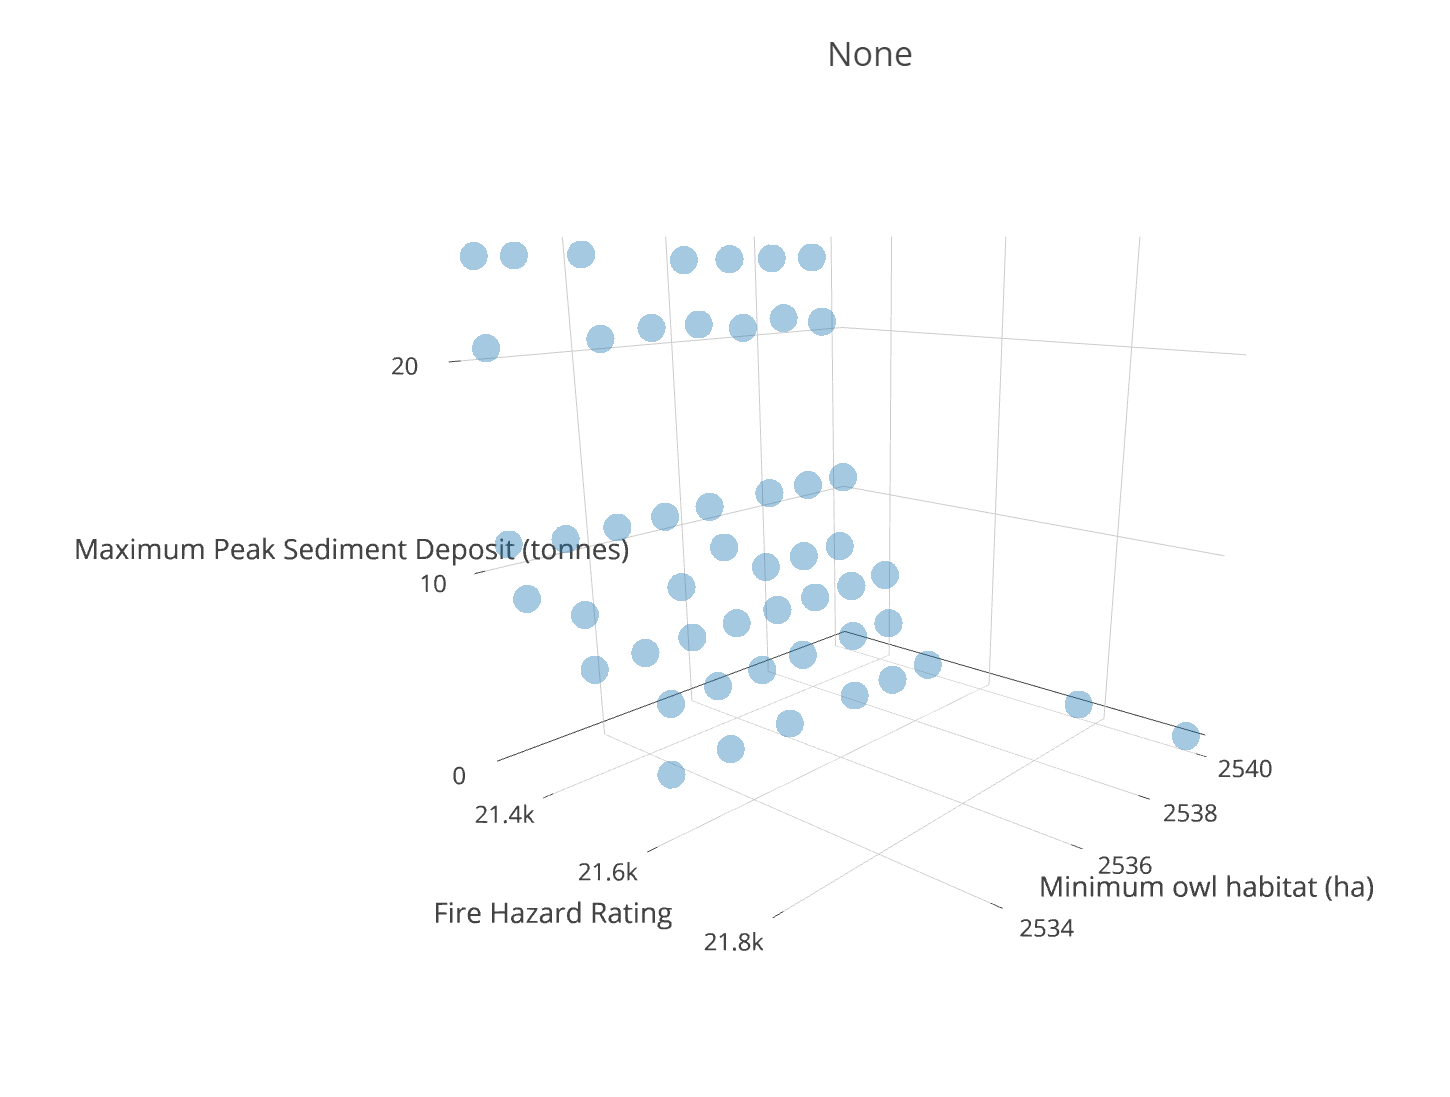
\includegraphics[width=.49\textwidth]{../images/Frontier_None}%
    \label{fig:frontierNone}%
  }
  \subfloat[Ensemble RCP 4.5]{%
    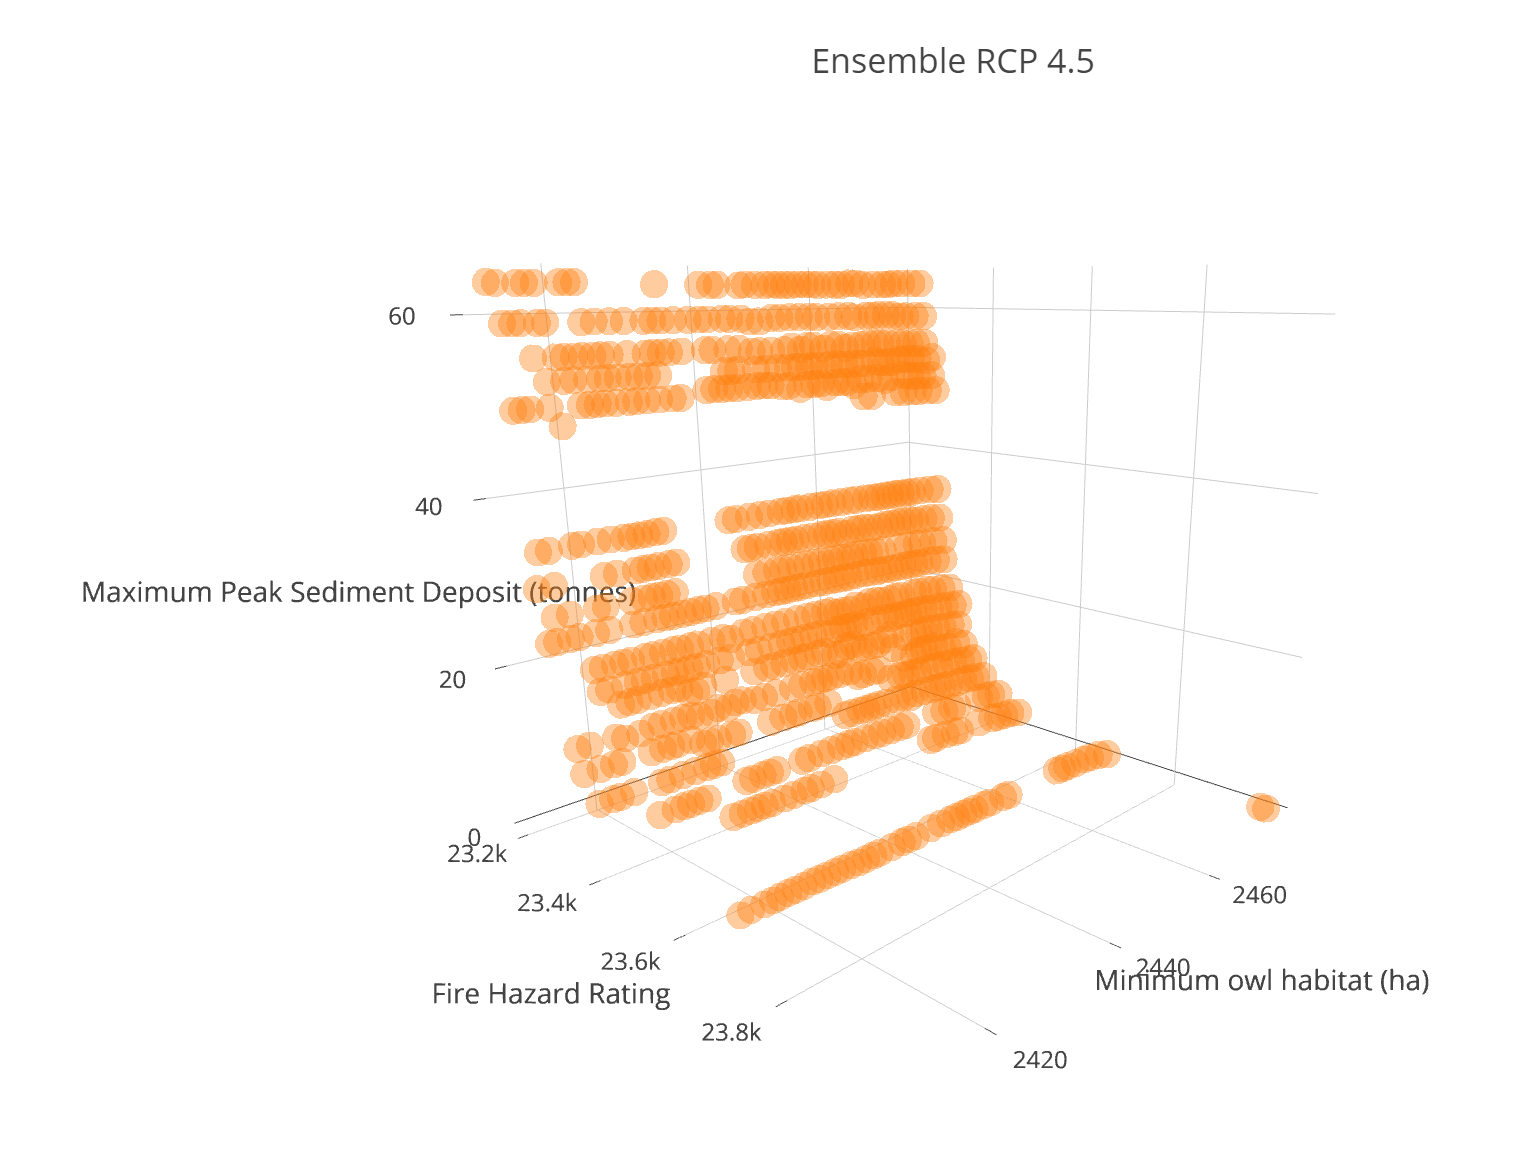
\includegraphics[width=.49\textwidth]{../images/Frontier_E45}%
    \label{fig:frontierE45}%
  }\hfill\centering
  \subfloat[Ensemble RCP 8.5]{%
    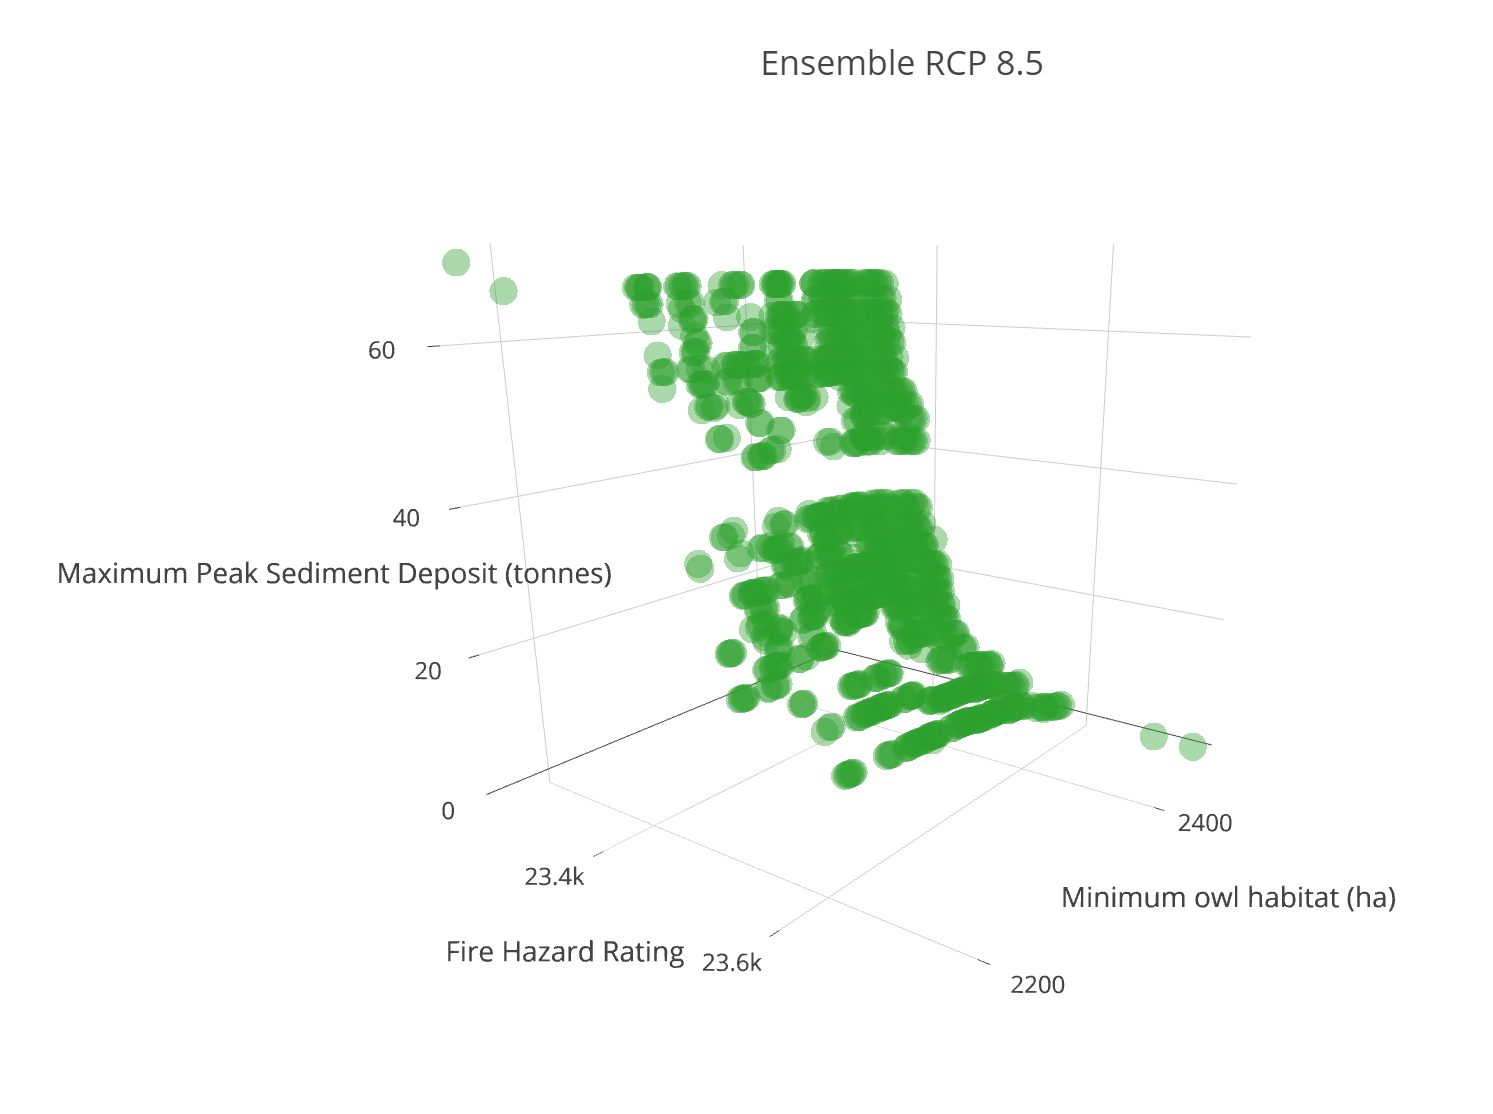
\includegraphics[width=.49\textwidth]{../images/Frontier_E85}%
    \label{fig:frontierE85}%
  }
  \caption[Frontiers for each climate change scenario]{Efficient frontiers for each climate change scenario.}
  \label{fig:frontiersAll}
\end{figure}

\begin{figure}[ht]
\centering
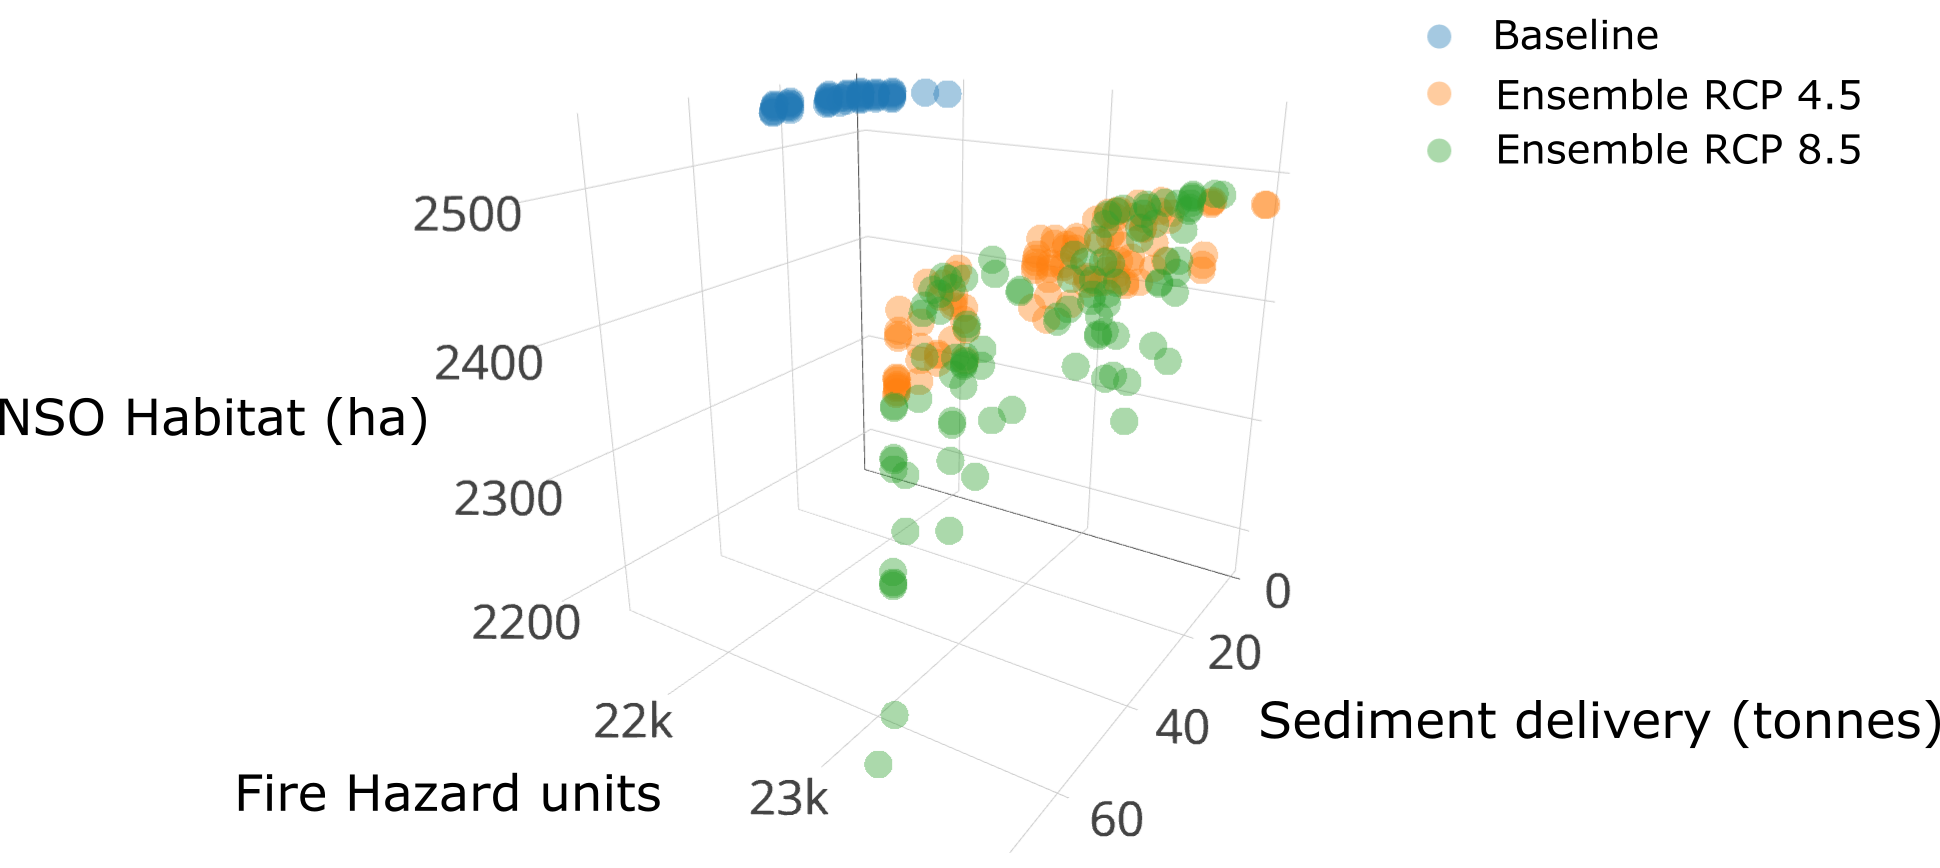
\includegraphics[width=.65\textwidth]{../images/consolidated3DFrontiers}
\caption[Unscaled 3D frontiers for all climate change scenarios]{Unscaled 3D frontiers for all climate change scenarios.}
\label{fig:consolidatedFrontiers}
\end{figure}

\begin{figure}[ht]
\centering
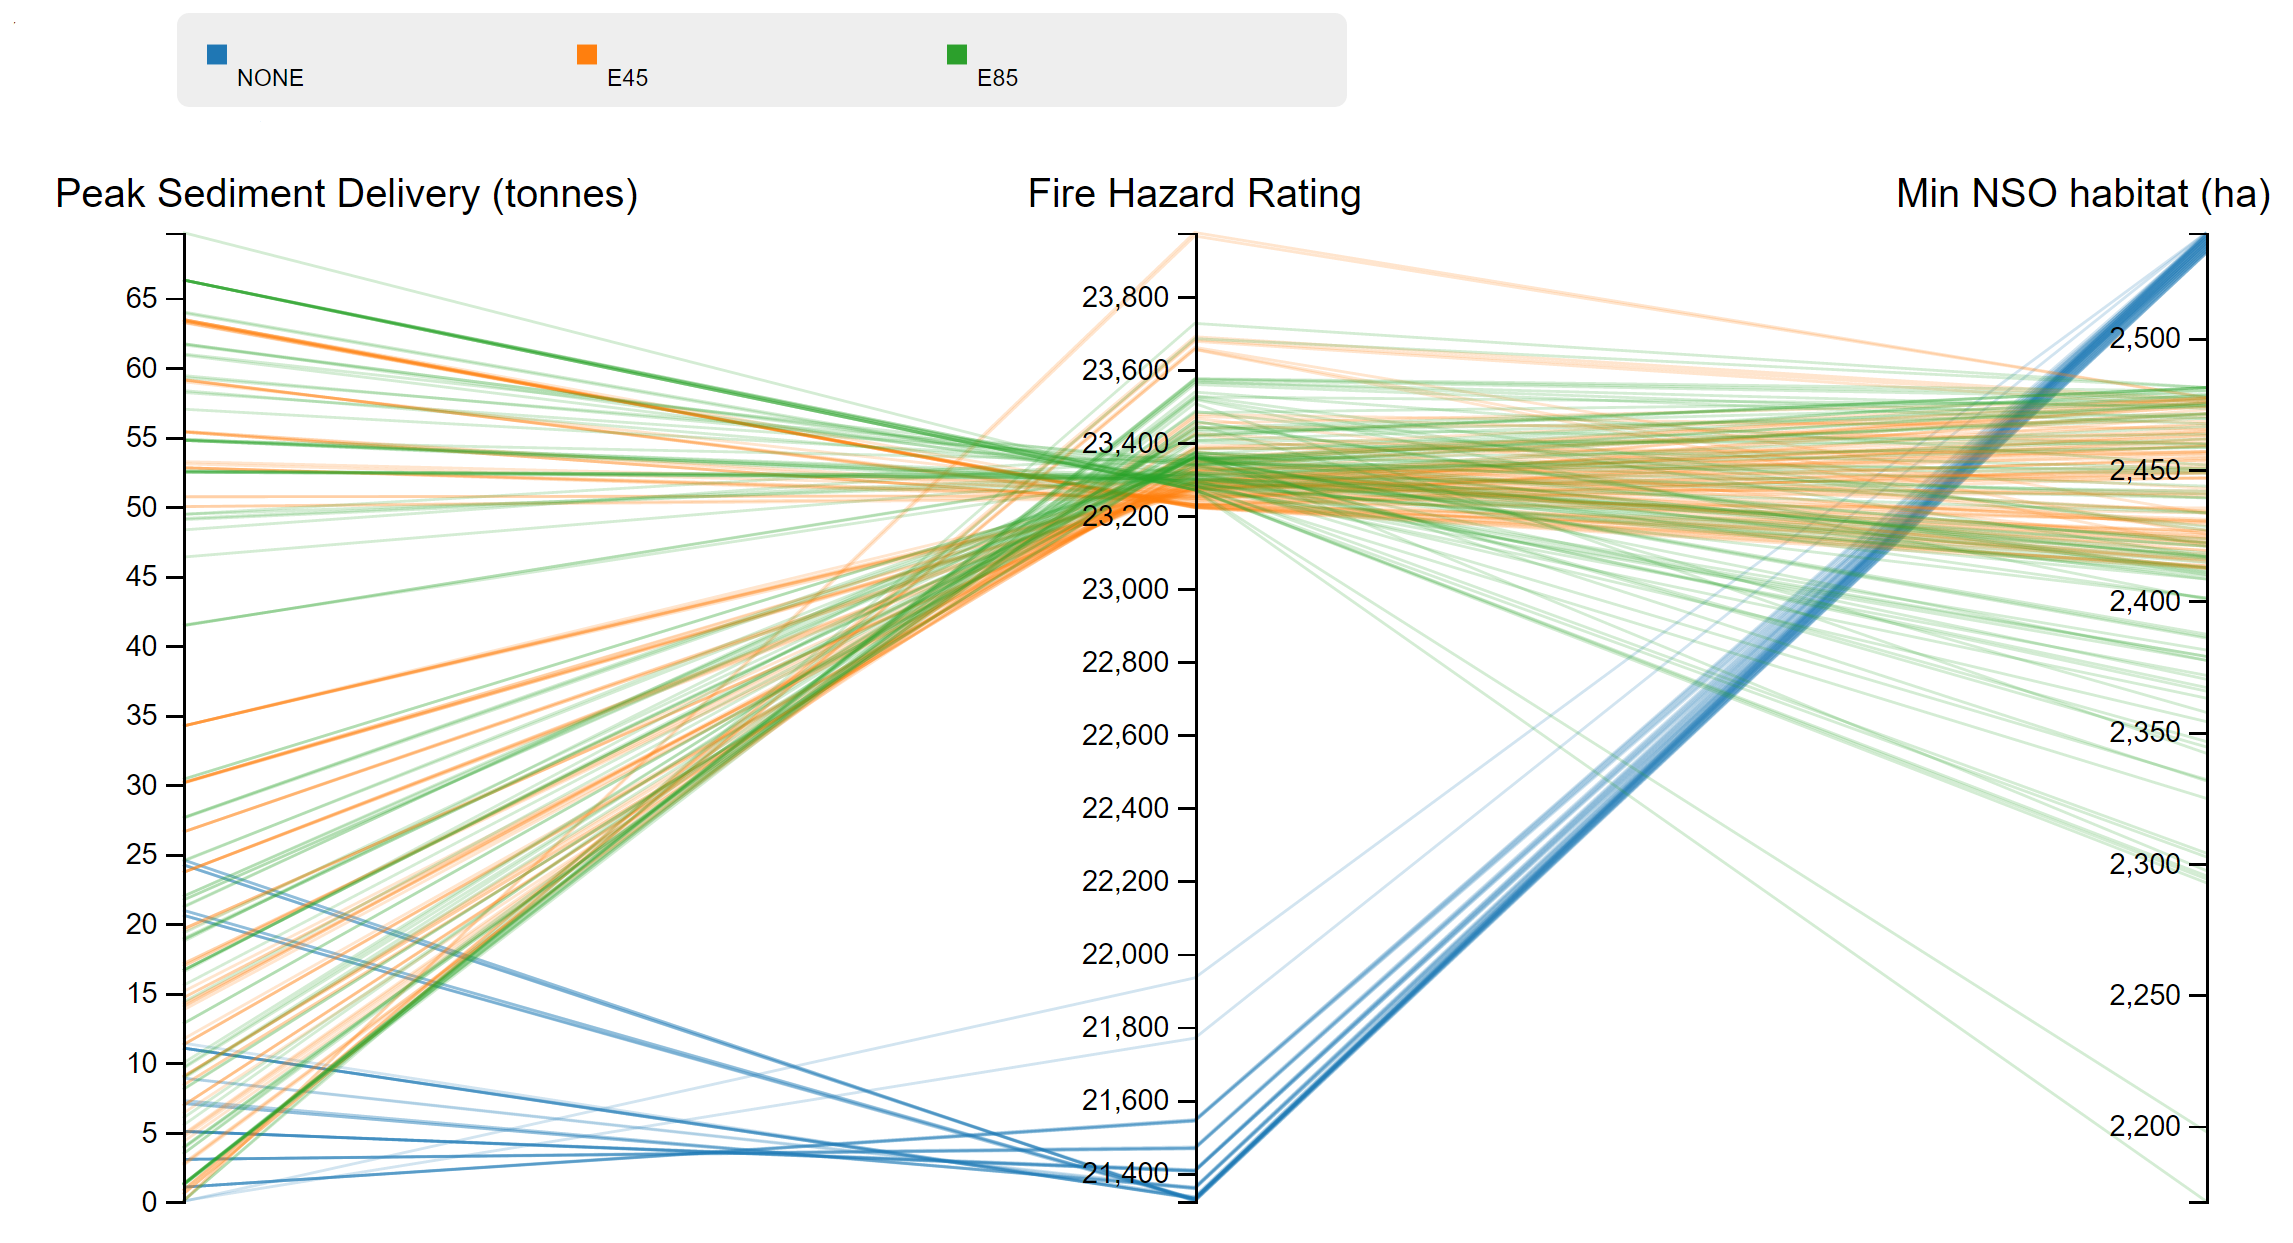
\includegraphics[width=.85\textwidth]{../images/FrontiersPCPlot}
\caption[Parallel coordinates view of the three frontiers]{Parallel coordinates view of the frontiers. Each axis represents an ecosystem service optimized by the model and each line represents a solution. In all objectives, we notice that None appears to outperform both the E45 and E85 scenarios, which show similar average objective achievements. To increase visual clarity, only a subset of solutions for E45 and E85 are shown.}
\label{fig:frontiersPCPlot}
\end{figure}

%We first report the impacts of climate change on the provision of individual ecosystem services before analyzing its impacts on the joint provision of ecosystem services and the conflict among them.

\subsection{Individual provision of ecosystem services}
The average achievement of all ecosystem services decreases with increasing severity of climate change -- see Table \ref{tab:frontiersSummary}. We find that the difference in ecosystem service provision is greater between the assumption of no climate change and mild climate change (None to E45) than it is between mild climate change and severe climate change (E45 to E85).

\paragraph{Sediment delivery} 
All scenarios have a lower bound on sediment delivery of 0, but the upper bound and the average sediment delivery both increase with climate change severity. Compared to the None scenario with an average sediment delivery of 10.25 tonnes, the average amount of sediment delivered in E45 is 27.98 tonnes, an increase of 172\%. The average for E85 is 31.19 tonnes, 204\% higher than None.

\paragraph{Fire hazard}
Similarly, we find that the average fire hazard of the Drink Area increases with climate change severity. The average for None is 21406.26 while E45 and E85 both perform approximately 9\% worse with an average of 23324.41 and 23369.57, respectively. This increase of 9\% in fire hazard is equivalent to the situation in which more than 1900 ha of the Drink area saw its fuel model raise from 5 to 13.

\paragraph{NSO habitat}
Finally, we also observe a decrease in the average provision of NSO habitat with increasing climate change. Compared to None which has an average provision of 2536.31 ha of NSO habitat, the average provision in the E45 scenario is 88.4 ha less (-3.5\%), and E85 is 114.3 ha less (-4.5\%).

We also find that for the sediment delivery and NSO habitat objectives, the range of achievable values increases with climate change severity. For sediment delivery, the range increases from 24.57 tonnes in None to 63.43 in E45 to 69.68 in E85. And for NSO habitat, the range increases from 7.72 ha in None to 65 ha in E45 and to 309.91 ha in E85.

\subsection{Conflict and the joint provision of ecosystem services}
As we saw for provision of individual ecosystem services, our results show that climate change will have an impact on conflict and the joint provision of ecosystem services as well.

We observe a decreasing hypervolume indicator with increasing severity of climate change -- see Table \ref{tab:hypervols}. The hypervolume for E45 is $0.0101$ less than None, and E85 is $0.0474$ less than None. However, all hypervolumes indicate frontiers which fill a large percentage of the objective space, as the smallest value (E85) is $I_{H1}(Z_\text{E85}) = 0.8295$. The binary hypervolumes (see Table \ref{tab:binaryHypervols}) tend to align with the hypervolumes, with larger values of $I_{H2}(Z_1,Z_2)$ when $I_{H1}(Z_1) > I_{H1}(Z_2)$ and smaller values when $I_{H1}(Z_2) > I_{H1}(Z_1)$. We note that no frontier is dominated by any other, as all binary hypervolume values in Table \ref{tab:binaryHypervols} are strictly positive.

\begin{table}[]
\centering
\caption[Hypervolumes of the efficient frontiers]{Hypervolume for each climate change scenario. Hypervolume values increase with increasing severity of climate change.}
\label{tab:hypervols}
\begin{tabular}{lllll}
\multicolumn{2}{l}{}                                                  & \textbf{None} & \textbf{E45} & \textbf{E85} \\ \hline
\multicolumn{2}{l}{\textbf{Hypervolume}}                              & 0.876977      & 0.866857     & 0.829541       
\end{tabular}
\end{table} 

\begin{table}[]
\centering
\caption[Binary hypervolume values for each pair of climate scenarios]{Binary hypervolumes for each pair of climate scenarios. No values are negative, indicating that no frontiers are dominated by another and that all frontiers uniquely enclose some volume of the objective space.}
\label{tab:binaryHypervols}
\begin{tabular}{lll}
\textbf{$Z_1$} & \textbf{$Z_2$} & \textbf{$I_{H2}(Z_1,Z_2)$} \\ \hline
\textbf{None}  & \textbf{E45}   & 0.026154                   \\
\textbf{None}  & \textbf{E85}   & 0.058001                   \\
\textbf{E45}   & \textbf{None}  & 0.016034                   \\
\textbf{E45}   & \textbf{E85}   & 0.045156                   \\
\textbf{E85}   & \textbf{None}  & 0.010565                   \\
\textbf{E85}   & \textbf{E45}   & 0.007841                  
\end{tabular}
\end{table}

\paragraph{Sediment delivery-NSO Habitat}
In the pairwise comparison of objectives, we observe little conflict between sediment delivery and NSO habitat under all climate scenarios. This is evident first in the proposed conflict metric $C_{ij}$, for which the largest value across all frontiers is 0.25 -- see Table \ref{tab:pairConflict-SedNSO}. We also notice the lack of conflict in Figure \ref{fig:pairplotNSOSed}. The figure shows the efficient frontier plotted in the sediment delivery-NSO habitat plane, where each objective has been normalized such that better values are higher and worse values are lower. For instance, in this graph, the point $(1,1)$ represents 0 sediment delivery and maximum NSO habitat. For all climate scenarios, we see similar uniform spreads of solutions as well as multiple solutions near the sub-dimensional ideal solution at $(1,1)$.

\begin{table}[]
\centering
\caption[Sediment-NSO conflict across climate scenarios]{Conflict between sediment delivery and NSO habitat across climate scenarios.}
\label{tab:pairConflict-SedNSO}
\begin{tabular}{llll}
\textbf{}     & \textbf{$C_{ij}$} & \textbf{$c_{ij,\rho}$} & \textbf{$c_{ij,d}$} \\ \hline
\textbf{None} & 0.19639           & 0.3974                 & 0.4942              \\
\textbf{E45}  & 0.25667           & 0.5194                 & 0.4941              \\
\textbf{E85}  & 0.19284           & 0.5160                 & 0.3737             
\end{tabular}
\end{table}


\begin{figure}[ht]
\centering
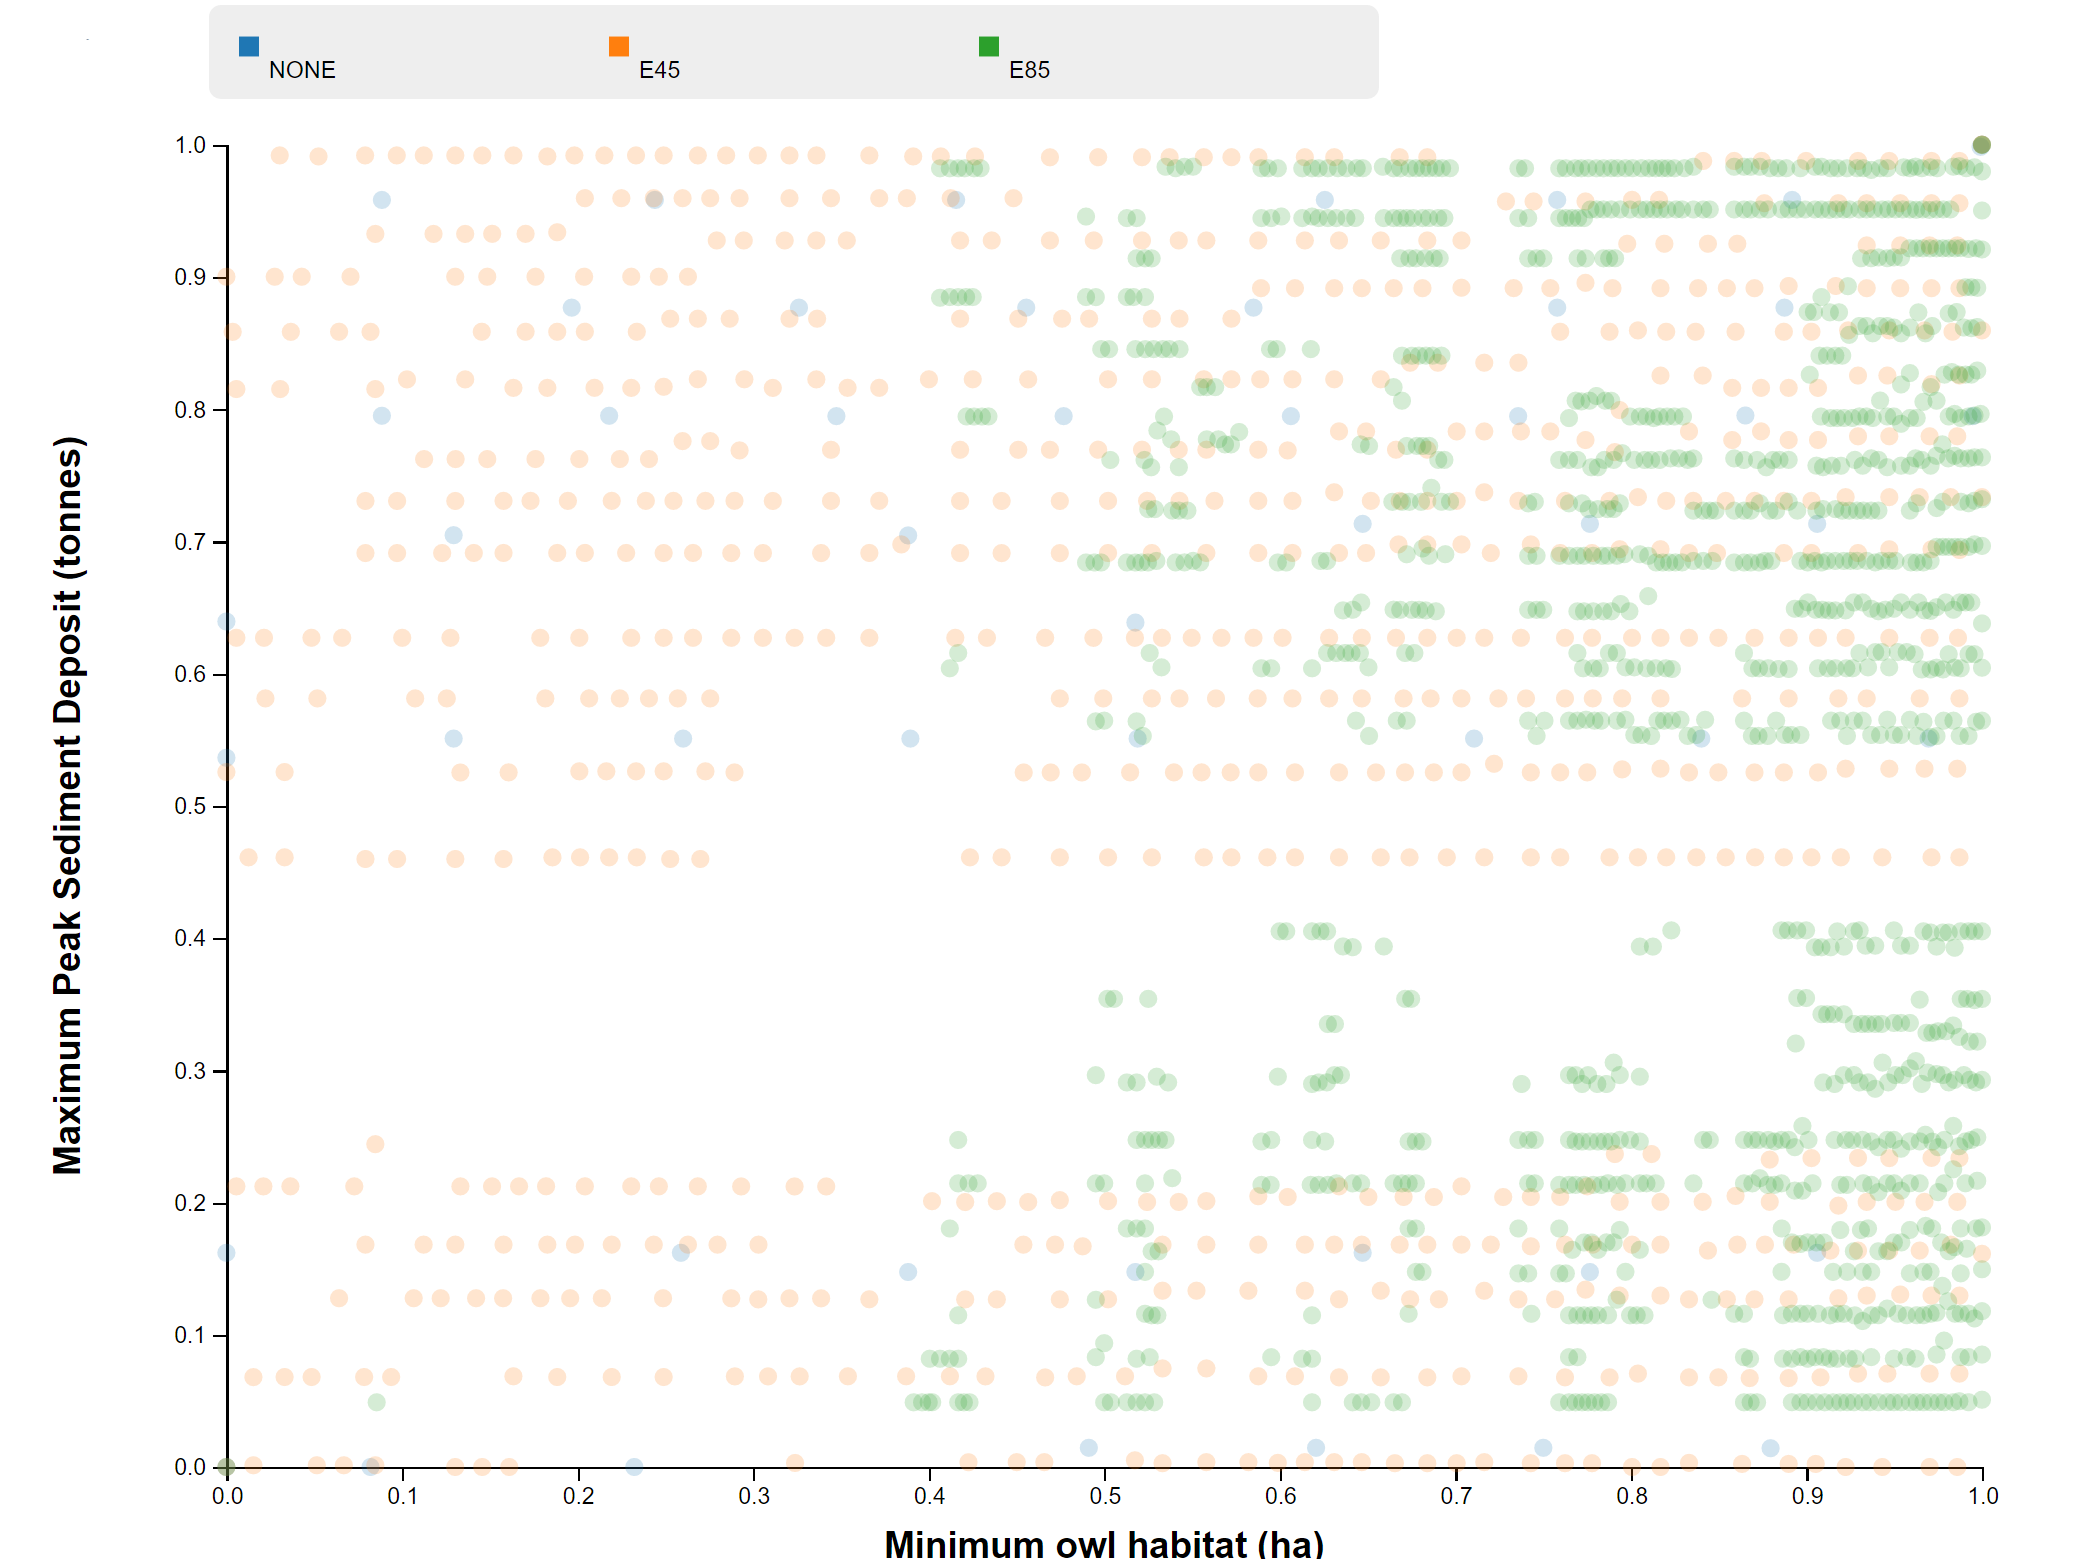
\includegraphics[width=.75\textwidth]{../images/2DSlice_NSO_Sed}
\caption[NSO habitat vs. sediment delivery for all climate scenarios]{NSO habitat versus sediment delivery for all climate scenarios. No obvious conflict pattern exists between the objectives in any climate scenario.}
\label{fig:pairplotNSOSed}
\end{figure}

\paragraph{NSO habitat-fire hazard}
According to $C_{ij}$, the conflict between NSO habitat and fire hazard is again small for all climate scenarios; however, it appears to decrease with increasing severity of climate change. We see in Table \ref{tab:pairConflict-NSOFire} that the average distance to the ideal decreases with increasing severity of climate change. See also Figure \ref{fig:pairplotNSOFire} which shows spreads of solutions for each climate scenario in the NSO habitat-fire hazard plane. The solutions are increasingly more clustered near the sub-dimensional ideal solution with increasing climate change severity.

\begin{figure}[ht]
\centering
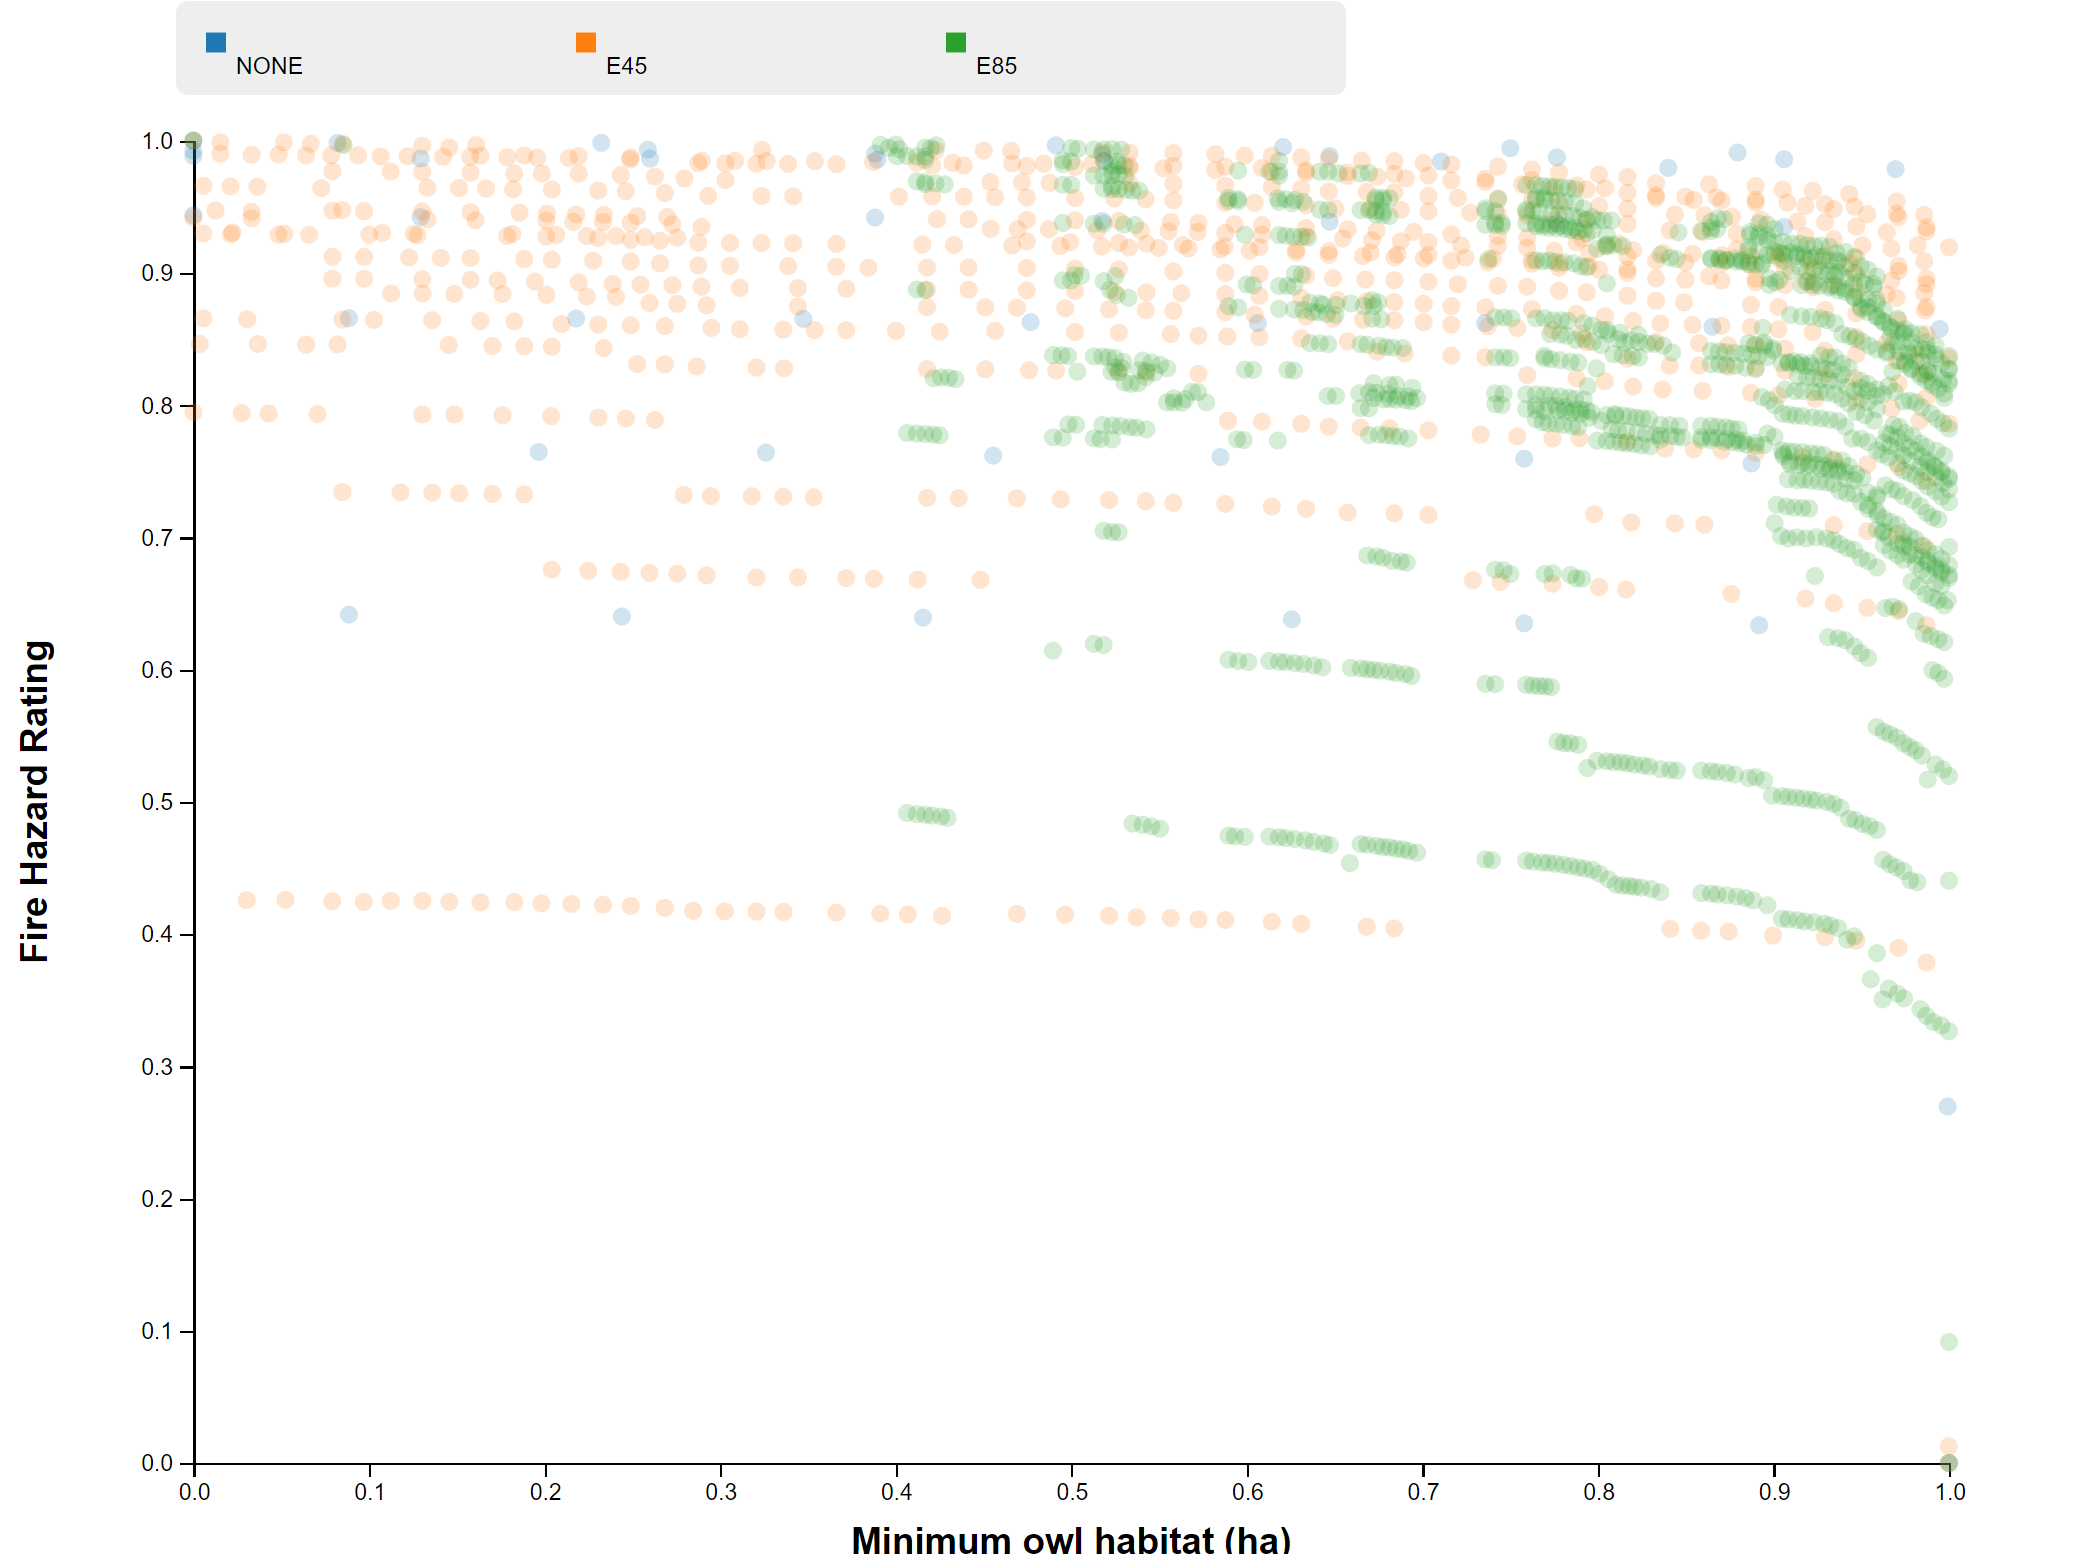
\includegraphics[width=.75\textwidth]{../images/2DSlice_NSO_Fire}
\caption[NSO habitat vs. fire hazard for all climate scenarios]{NSO habitat versus fire hazard for all climate scenarios.}
\label{fig:pairplotNSOFire}
\end{figure}

\begin{table}[]
\centering
\caption[NSO-fire hazard conflict across climate scenarios]{Conflict between NSO habitat and fire hazard across climate scenarios.}
\label{tab:pairConflict-NSOFire}
\begin{tabular}{llll}
\textbf{}     & \textbf{$C_{ij}$} & \textbf{$c_{ij,\rho}$} & \textbf{$c_{ij,d}$} \\ \hline
\textbf{None} & 0.25805           & 0.6622                 & 0.3897              \\
\textbf{E45}  & 0.20560           & 0.5807                 & 0.3541              \\
\textbf{E85}  & 0.15670           & 0.6643                 & 0.2359
\end{tabular}
\end{table}

\paragraph{Fire hazard-sediment delivery}
In all climate scenarios, the strongest pairwise conflict is between fire hazard and sediment delivery. This is apparent from both Figure \ref{fig:pairplotSedFire} and the conflict metric, Table \ref{tab:pairConflict-SedFire}. All rank correlation conflict values $c_{ij,\rho} > 0.95$, indicating strong negative rank correlation. In Figure \ref{fig:pairplotSedFire} we observe a clear void of solutions in all climate change scenarios near the sub-dimensional ideal solution at $(1,1)$; this is unlike Figures \ref{fig:pairplotNSOSed} and \ref{fig:pairplotNSOFire}. We also notice that the None and E45 solutions generally extend beyond the E85 solutions in this plane.

\begin{figure}[ht]
\centering
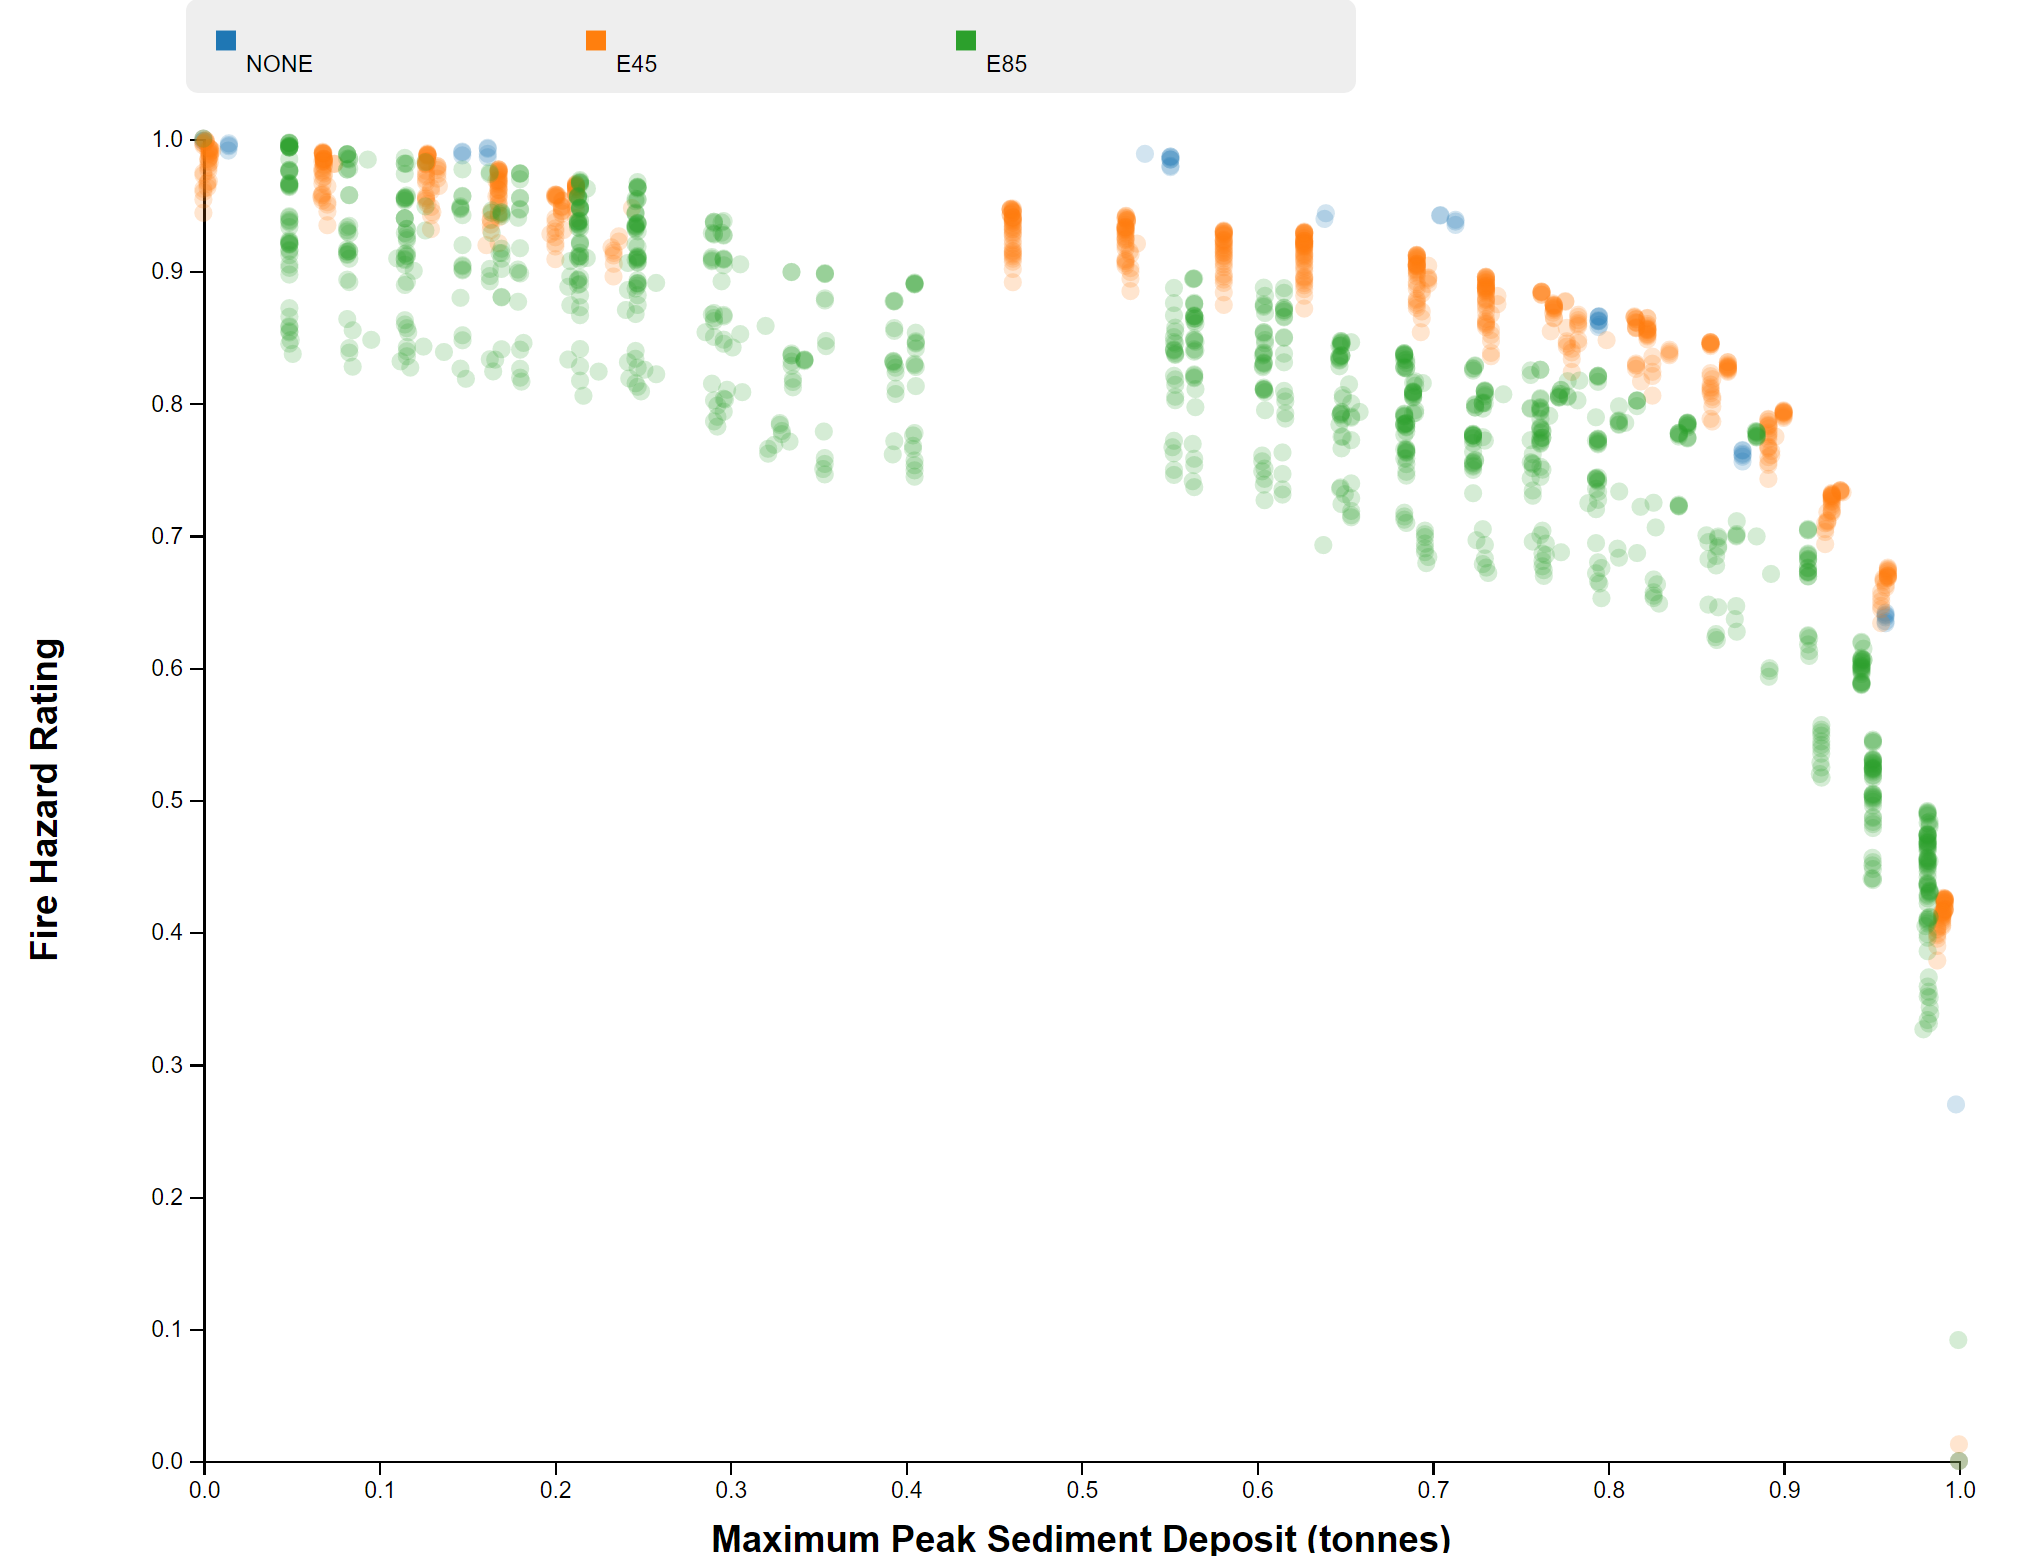
\includegraphics[width=.75\textwidth]{../images/2DSlice_Sed_Fire}
\caption[Sediment delivery vs. fire hazard for all climate scenarios]{Sediment delivery versus fire hazard for all climate scenarios.}
\label{fig:pairplotSedFire}
\end{figure}

\begin{table}[]
\centering
\caption[Sediment delivery-fire hazard conflict across climate scenarios]{Conflict between sediment delivery and fire hazard across climate scenarios.}
\label{tab:pairConflict-SedFire}
\begin{tabular}{llll}
\textbf{}     & \textbf{$C_{ij}$} & \textbf{$c_{ij,\rho}$} & \textbf{$c_{ij,d}$} \\ \hline
\textbf{None} & 0.36039           & 0.9927                 & 0.3630              \\
\textbf{E45}  & 0.36097           & 0.9853                 & 0.3664              \\
\textbf{E85}  & 0.38261           & 0.9514                 & 0.4021
\end{tabular}
\end{table}

\section{Discussion}
We divide our discussion of results into three sections: first, the decreasing provision of individual ecosystem services with climate change; second, the increase in the number of solutions; and third, conflict and the joint provision of ecosystem services.

\subsection{Decreasing provision of individual ecosystem services}
We observe decreasing provision of individual ecosystem services with increasing severity of climate change. In particular, we see that the difference between no climate change (None) and mild climate change (E45) was greater than the difference between mild climate change (E45) and severe climate change (E85). Refer to Table \ref{tab:frontiersSummary}. This suggests that, at least for the ecosystem services in this study, the realization of climate change is more significant than the severity of that change.

\paragraph{Sediment delivery}
Investigating the cause of the degradation in sediment delivery, we find that the average spike in sediment delivered as a result of performing a fuels treatment increases with climate change. See Figure \ref{fig:avgSedimentDelivery}. The average sediment delivery per fuel removal under E45 is nearly twice the sediment delivery under the None scenario (81\% higher), and the E85 scenario is 0.4\% higher than that. This is driven by two underlying factors: the response in sediment delivery to prescribed burns and the frequency with which prescribed burns are assigned\footnote{For additional information on how treatment units are assigned a specific fuel removal technique such as thinning or prescribed burn, see the appendix, \S \ref{chap:appendix_drinkTreatments}.}. Our simulations show that increasing the severity of climate change causes pronounced increases in sediment delivery as a result of prescribed burns. We also find that relative to the None scenario, prescribed burns are assigned more frequently in the climate change scenarios -- 8 times more frequently in E45 and 10.1 times more frequently in E85. See Table \ref{tab:prscBurnsInClimChange}. These effects combine to produce the result seen in Figure \ref{fig:avgSedimentDelivery} of sediment delivery levels that increase with climate change severity.

\begin{figure}[ht]
\centering
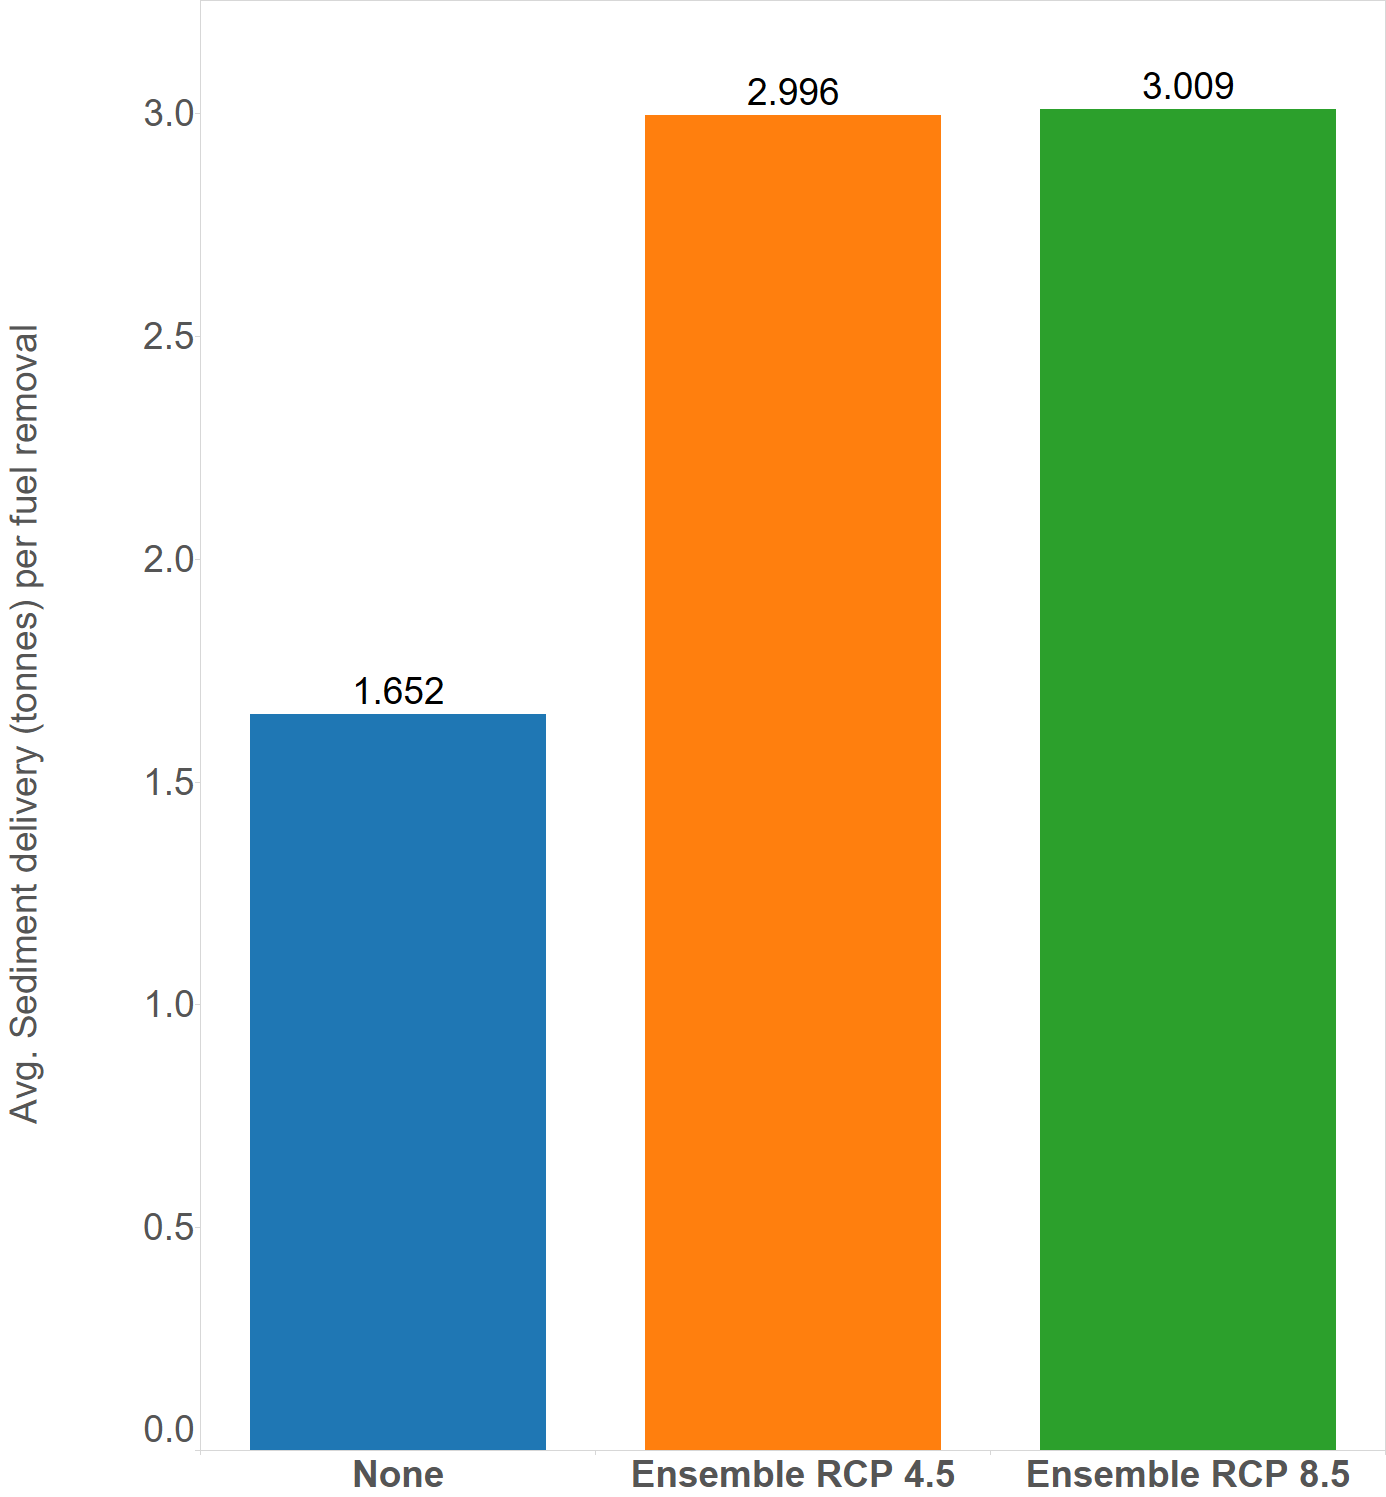
\includegraphics[width=.55\textwidth]{../images/AvgSedimentSpikes}
\caption[Average sediment delivery across climate scenarios]{Average spike in sediment delivery as a result of performing fuel removals for each climate change scenario.}
\label{fig:avgSedimentDelivery}
\end{figure}

\begin{table}[]
\centering
\caption[Frequency and impact of prescribed burns across climate scenarios]{Frequency and impact of prescribed burns for each climate scenario. The combination of more frequent prescribed burns and increased sediment delivery per prescribed burn results in the higher values of sediment delivery in E45 and E85 observed in Figure \ref{fig:avgSedimentDelivery}.}
\label{tab:prscBurnsInClimChange}
\begin{tabular}{llll}
                                                                                                           & \textbf{None} & \textbf{E45} & \textbf{E85} \\ \hline
\textbf{\begin{tabular}[c]{@{}l@{}}Average sediment delivery\\ (tonnes) from prescribed burn\end{tabular}} & 31.23            & 48.56          & 48.97          \\
\textbf{\begin{tabular}[c]{@{}l@{}}Number of prescribed\\ burns assigned\end{tabular}}                     & 34         & 272        & 344       
\end{tabular}
\end{table}

\paragraph{Fire hazard}
For the fire hazard objective, recall that we constrain the total area treated in each period. We first note that the increase in fire hazard with climate change severity is not simply due to the model selecting less area for treatment. Across both treatment periods and all climate scenarios, the model consistently utilizes over 99\% of the allowable value -- see Table \ref{tab:treatedAreas}. Instead, we find that the increase in fire hazard is due to the impact of climate change on the fuel model classification of the treatment units in the Drink Area. In E45 and E85, more treatment units are assigned a fuel model classification that is associated with higher fire hazard (refer to Table \ref{tab:firehazards} for the mapping from fuel models to fire hazard). This is shown in Figure \ref{fig:distOfFireHazards}, where we observe a larger percentage of treatment units having a fire hazard rating of either 4 or 5 under the E45 and E85 scenarios than in None.

\begin{table}[]
\centering
\caption[Area treated per period across climate scenarios]{Areas treated per period across climate scenarios. The values are nearly constant for both periods and for each climate scenario.}
\label{tab:treatedAreas}
\begin{tabular}{llll}
                                                                                                           & \textbf{None} & \textbf{E45} & \textbf{E85} \\ \hline
\textbf{Area treated (ha) in period 1} & 2427.31            & 2426.90 & 2414.58          \\
\textbf{Area treated (ha) in period 2}                     & 2427.56         & 2427.71        & 2427.63      
\end{tabular}
\end{table}

\begin{figure}[ht]
\centering
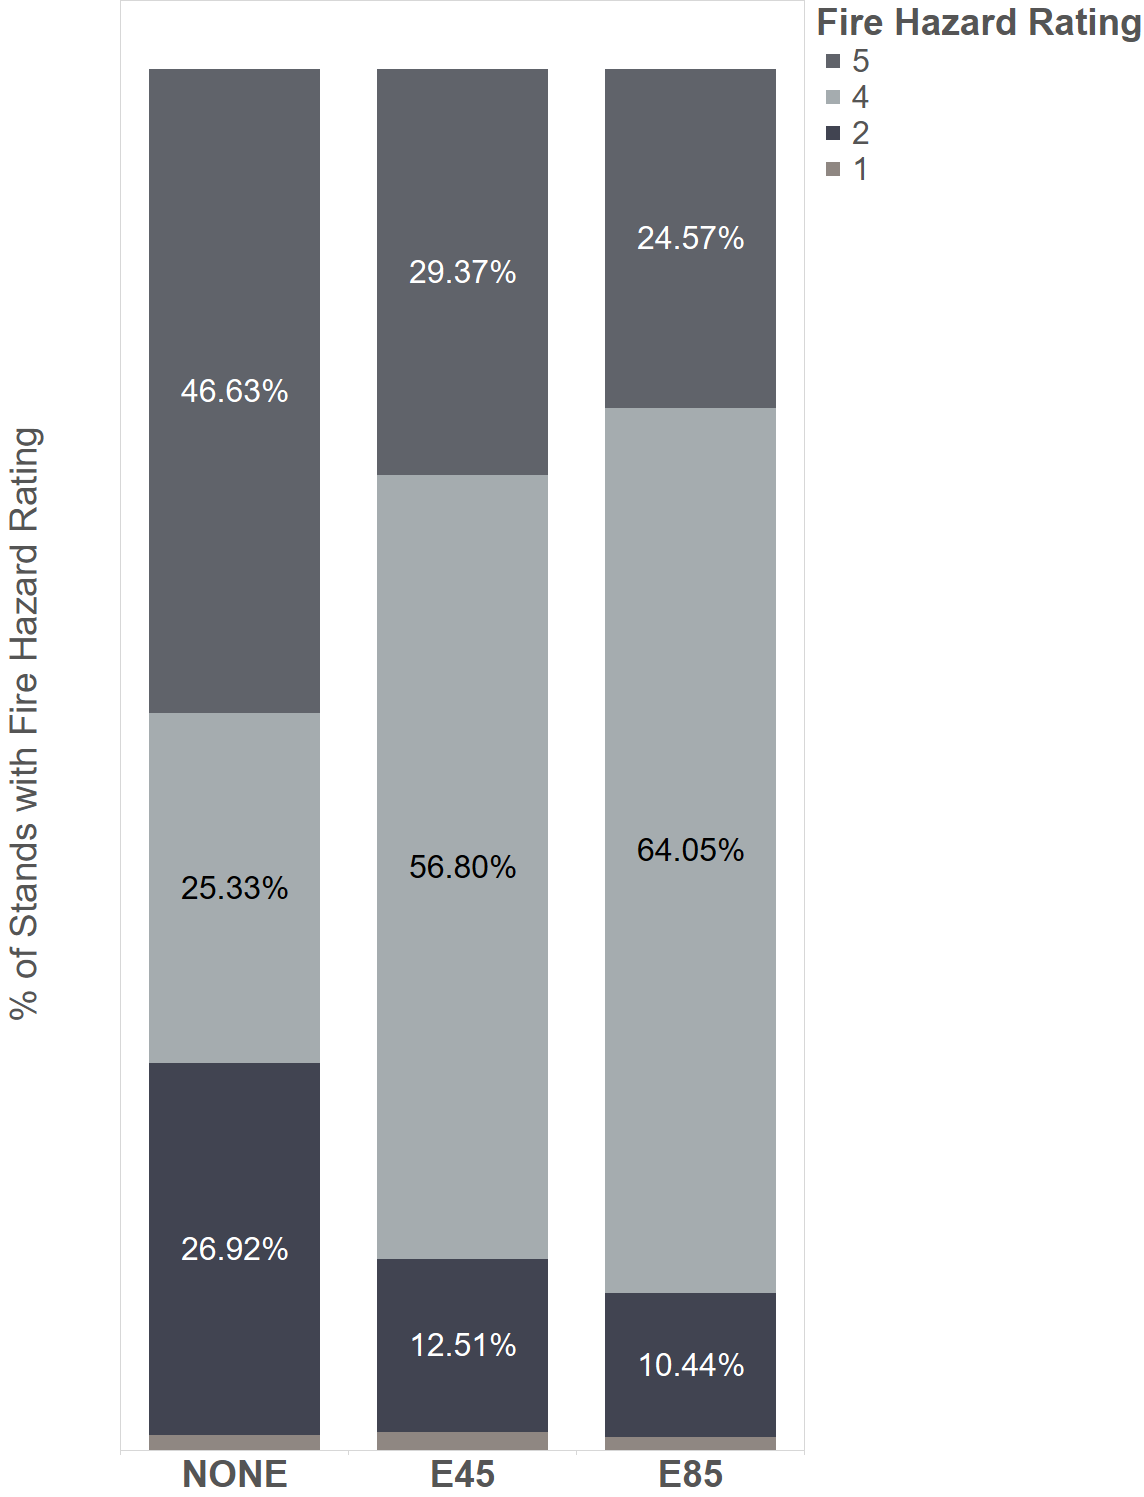
\includegraphics[width=.5\textwidth]{../images/FireHazardRatingsPerClimateScenario}
\caption[Distribution of fire hazard ratings over the Drink Area for each climate change scenario]{Distributions of fire hazard ratings across the Drink Area under each climate change scenario. Moving from left to right (in increasing climate change severity), we observe an increase in the percent of treatment units classified with more extreme fire hazards (ratings of 4 and 5).}
\label{fig:distOfFireHazards}
\end{figure}
% If we need a map, show a single map that shows the diff in FH at 2095 for a good sol from E85 - good sol from None

\paragraph{NSO habitat}
Lastly, we find that the decrease in NSO habitat is largely due to the effects of climate change on the vegetation in the Drink Area. Recall that of the criteria used to determine if a treatment unit qualifies as NSO habitat, two are determined by vegetation characteristics: the presence of at least one tree with DBH $> 76$ cm and canopy closure of at least 60\%. While climate change has minimal impact on the former, the average canopy closure for treatment units in the Drink Area decreases with increasing severity of climate change. See Figure \ref{fig:canopyClosure}.

\begin{figure}[ht]
\centering
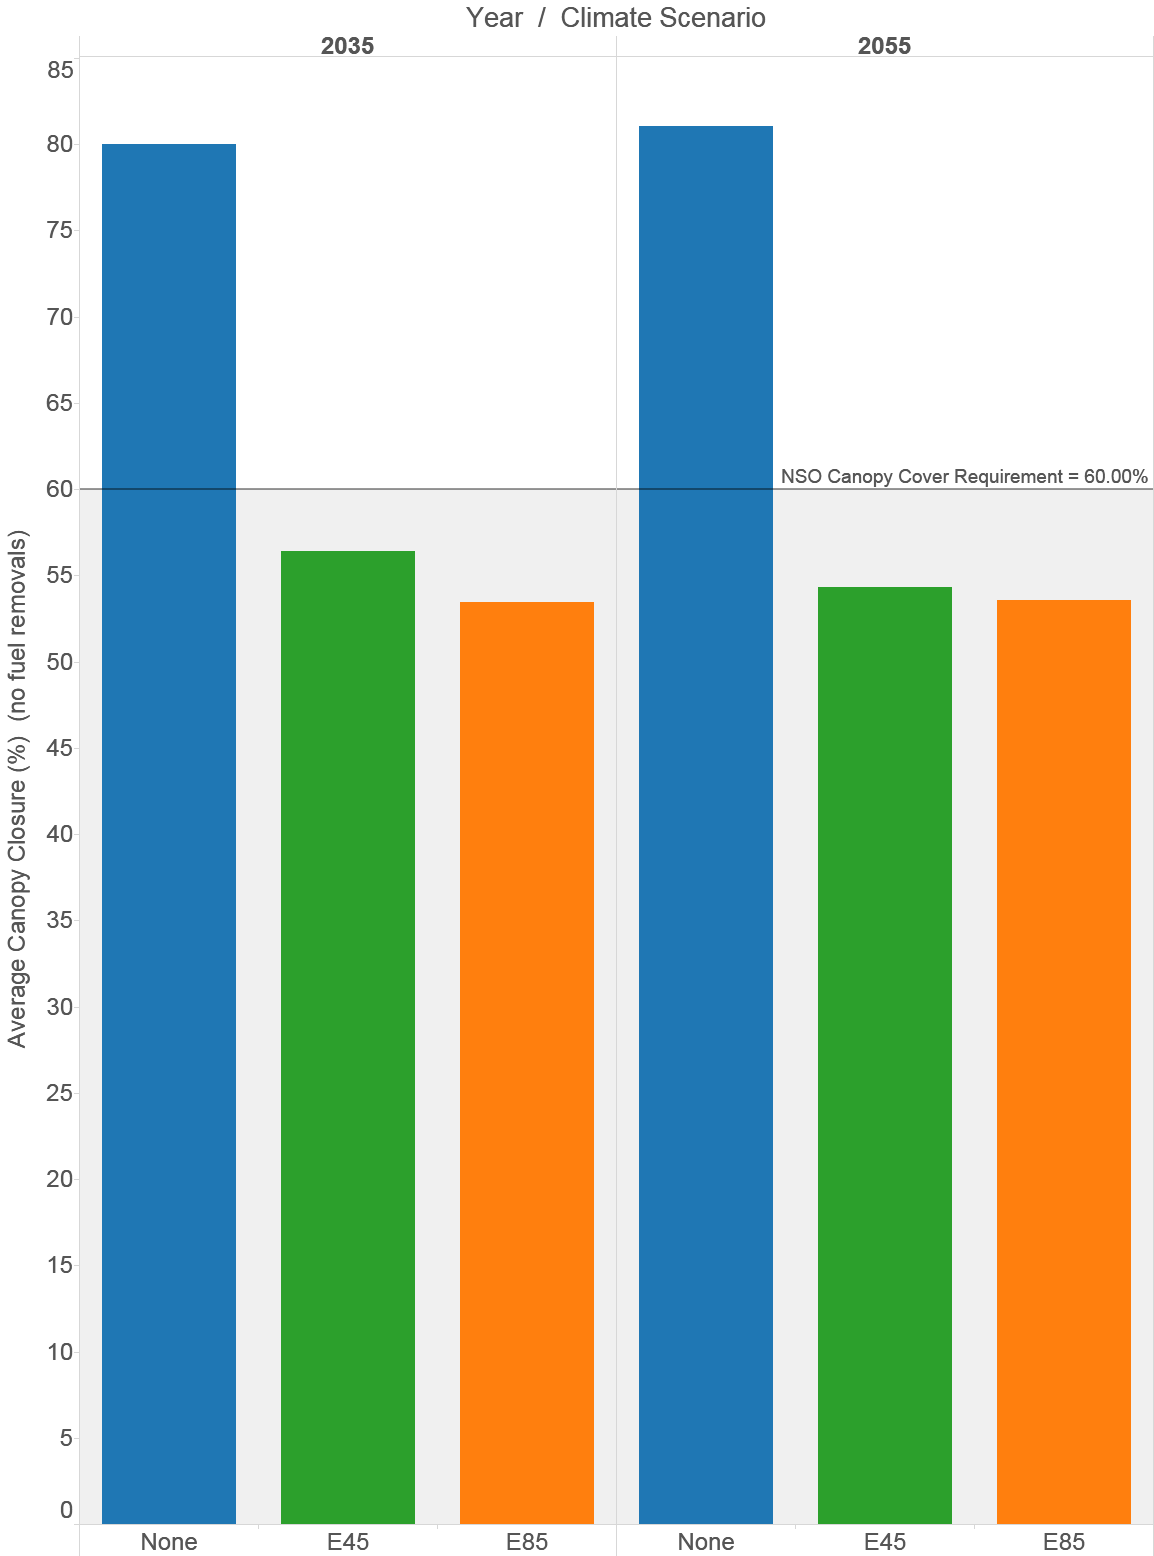
\includegraphics[width=.5\textwidth]{../images/AvgCanopyCover_NoTrtmts}
\caption[Average canopy closure in the Drink Area across climate scenarios]{Average canopy closure for treatment units in the Drink Area for each climate scenario. Shown are canopy closure values during years 2035 and 2055 (the years in which NSO habitat is measured) when no fuel removals are performed. We see that with increasing climate change severity, canopy closure decreases.}
\label{fig:canopyClosure}
\end{figure}


\subsection{Variation in number of solutions}
With increasing climate change severity, we noted an increase in the number of solutions generated by our model:  51 for $Z_{\text{None}}$, 701 for $Z_{\text{E45}}$, and 1083 for $Z_{\text{E85}}$. We suspect this is because fuel removals more frequently alter whether a treatment unit qualifies as NSO habitat in the climate change scenarios. This also drives the greater variation in NSO habitat seen for the E45 and E85 scenarios.

The number of instances in which performing a fuel removal disqualifies a treatment unit from being NSO habitat is 24 in None, 63 in E45, and 67 in E85. Let us refer to such fuel removals as ``disqualifying treatments.'' By more than doubling the number of disqualifying treatments in the E45 and E85 scenarios, additional solutions are produced in those frontiers. If these disqualifying treatments generated little fire hazard reduction in return for the disqualification of NSO habitat, then these decisions would not be part of the optimal solutions $\mathbf{x} \in P$. However, we find that the reduction in fire hazard for a given disqualifying treatment increases with climate severity (Figure \ref{fig:nsoHabDQFHEfficacy}). This leads to greater incentive for the model to sacrifice NSO habitat in favor of fire hazard reduction.

\begin{figure}[ht]
\centering
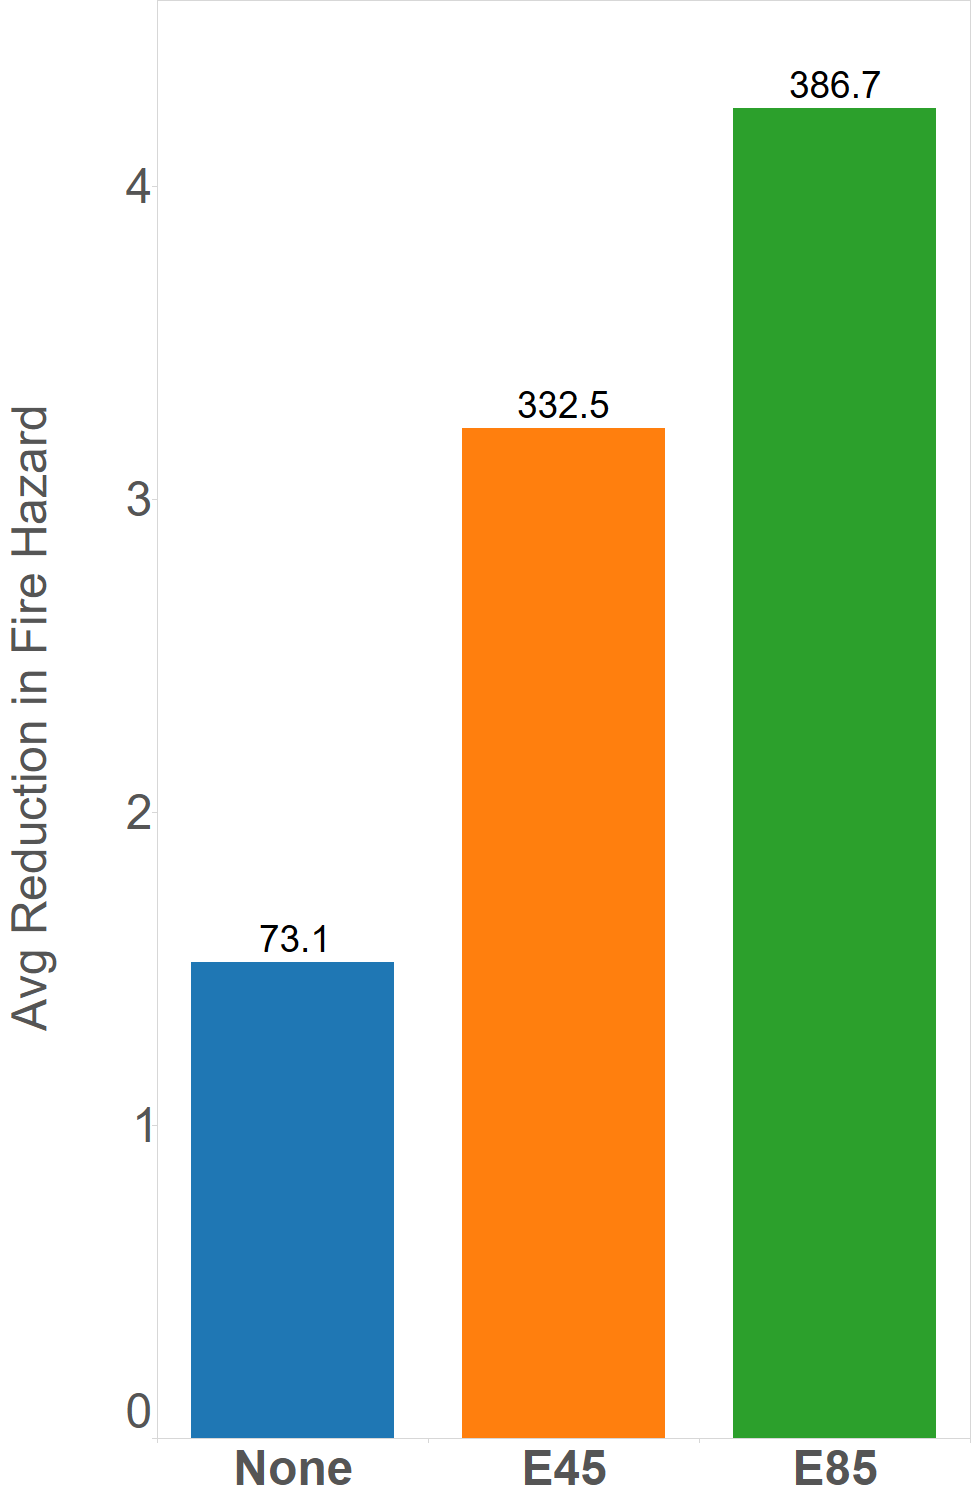
\includegraphics[width=.5\textwidth]{../images/AvgFireHazardEffectivenessForNSODQs}
\caption[Efficacy of fuel removals for NSO habitat disqualification]{Some treatment units may always be NSO habitat and others may never be NSO habitat, regardless of model decisions. For those treatment units which vary based on model decisions, we see here the average efficacy of fuel removals which disqualify their being NSO habitat. This value increases with increasing climate change, indicating greater incentive for the model to forgo NSO habitat in favor of fire hazard reduction.}
\label{fig:nsoHabDQFHEfficacy}
\end{figure}

Together, these factors lead to an increase in the number of solutions as well as greater variation in the total amount of NSO habitat provided by the models.

\subsection{Conflict and the joint provision of ecosystem services}
We observe a decreasing hypervolume with increasing climate change severity. Lower values for the hypervolume are indicative of more conflict, meaning that climate change induces more conflict among the ecosystem services and leads to less joint provision of objectives.

The difference in hypervolume between None and E45 $I_{H1}(Z_\text{None}) - I_{H1}(Z_\text{E45}) \approx 0.01$. Recall that a difference of $h$ in hypervolumes equates to a difference of $h^{1/M}$ in each objective (Figure \ref{fig:Hypervol10percent}). Thus, despite the small size of the difference between $I_{H1}(Z_\text{None})$ and $I_{H1}(Z_\text{E45})$, the additional volume of the objective space bound by None signifies an additional joint provision of objectives of approximately 21.6\%. This difference means that there are solutions in None that represent an simultaneous improvement in each objective of more than 7\% over any solution in E45.  The difference in hypervolume indicators is greater between None and E85, approximately 0.05. This represents an additional joint provision of ecosystem services of approximately 36.2\% in None compared to E85, or an improvement in each objective of more than 12\%.

From the hypervolumes alone, it is uncertain whether None represents a strictly better frontier than either E45 or E85 or if, despite their smaller hypervolume values, E45 and E85 enclose some region of the objective space that is not enclosed by None. Any such region would extend further into the objective space, representing the presence of solutions that achieve greater joint provision of ecosystem services. The results of the binary hypervolume were presented in Table \ref{tab:binaryHypervols}.

The results show that no frontier is dominated by any other, and each frontier encloses some region of the objective space not enclosed by the others. For the pairs of frontiers for which the binary hypervolume is greatest ($(Z_\text{None},Z_\text{E85})$ and $(Z_\text{E45},Z_\text{E85})$), this additional extension into the objective space is most obvious in Figure \ref{fig:pairplotSedFire}. We see for values of sediment delivery between 0.15 and 0.8 that None appears to dominate E45 which appears to dominate E85. Further, for sediment delivery values between 0.8 and 1, it appears that E45 dominates E85 and None, between which any domination relationship is difficult to discern.

The existence of these areas leads to the lower value of conflict $C_{ij}$ between sediment delivery and fire hazard in None and E45 than in E85. We claim that this is a success of the conflict metric $C_{ij}$: all frontiers in the sediment delivery-fire hazard plane of Figure \ref{fig:pairplotSedFire} are similar. They have similar shape and achievement towards the sub-dimensional ideal solution, yet the metric is able to distinguish differences in conflict between them.

For the other pairwise objective comparisons, as we saw in Figures \ref{fig:pairplotNSOSed} and \ref{fig:pairplotNSOFire}, the distribution of solutions more closely resembles a uniform two-dimensional scattering. There is no clear conflict pattern between them similar to what we saw in Figure \ref{fig:pairplotSedFire}. As a result, $C_{ij}$ reports little conflict between these objective pairs. However it varied in unexpected ways between the climate scenarios. In these cases, we find that the distance component $c_{ij,d}$ was primarily responsible for the variations, as the rank correlations tended to be insignificantly different from 0.5. It appears the conflict metric $C_{ij}$ is susceptible to such variations when neither the $c_{ij,d}$ nor $c_{ij,\rho}$ component tends towards their limiting values of 0 and 1.

% In general, however, it was really awesome.
However, in general, we find our process of utilizing the hypervolume measures and the proposed conflict metric to have been successful in quantifying conflict within and among the frontiers. The pairwise conflict metric successfully identified the pair of objectives which demonstrated the most conflict, and the hypervolumes indicated which climate scenarios allow for greater joint provision of ecosystem services.

\section{Management implications}
The management implications of the findings of this case study largely entail required adaptations to climate change. The degradation in the individual and joint provision of ecosystem services means that the decision makers for the Drink Area may need to reevaluate the priorities given to these objectives. For instance, because in the case of climate change a given reduction in fire hazard requires a more substantial sediment delivery, forest managers may need to consider which of these objectives they are more comfortable compromising. Status quos will change, such as performing fire hazard reduction techniques and being comfortable with the resulting impacts on NSO habitat or watershed sediment content. Under climate change, we saw that fuel removal techniques are predicted to be simultaneously more intensive and less effective. If there are thresholds for the allowable levels of sediment delivery or NSO habitat, those may need to be revisited in light of the increased fire hazard required to exist within those thresholds.

Managers will benefit from an awareness of how the conflict among objectives is changing. Again, it allows them to reevaluate current thresholds on objectives and determine if those values are still sensible. It also may force managers to consider their objectives again and determine if some hold a higher priority than others. For instance, if sediment delivery and fire hazard become increasingly incompatible, which should be subject to a greater sacrifice in order to maintain more of the other? Further, while undiscussed here, each solution to these models captures a management plan, complete with the spatio-temporal information regarding fuel removals. By identifying similarities in management plans relative to a given objective achievement, it allows managers to identify which fuel removal practices are most robust across the climate scenarios. Similarly, it allows them to identify which fuel removal practices are least desired, resulting in an objective achievement deemed too poor for practical implementation.
\section{Discussion \& Conclusion}
% We did good
We used a case study of the impact of climate change on the joint provision of forest ecosystem services to successfully demonstrate the utility of a new measure of pairwise objective conflict and to demonstrate a new application of existing conflict measures in the quantification of conflict within and among multi-objective systems.

% We did good in something that was hard to do good in
A general lack of conflict between objectives and the similarity across climate scenarios considered in this case study make it a rigorous test of the utility of the existing and proposed conflict measures. In the case study, the hypervolumes for the climate scenarios were relatively large, with over 80\% of the objective space consistently occupied by solutions. In addition, in all but one pairwise objective comparison, it was difficult to discern any distinct conflict relationship between the objectives. Thus the new conflict metric was required to detect subtle difference in conflict, which we argue it did. Should the difference between scenarios have been more pronounced, or should the objectives have been in greater conflict with one another, we suspect the utility of the process we demonstrated here would only increase.

% But who's to say that it will always do good. It may not, but to check we need the tool, and that's what we came up with.
We saw that it worked for us, but the results may be different if under diff circumstances. But we need to be able to perform this sort of analysis, and that is why we came up with what we did. We showed that it was useful here.

% You might also look at this thing to see if it does good here
For instance, if a food processing facility HAD BLANK SOME LARGE SWEEPING MACHINE-TECH CHANGE, then BLANK WOULD HAPPEN AND OUR CONFLICT MEASURE WOULD BE GREAT TO DETECT THESE DIFFS.

% Or this other thing
Or if some regulatory change happened to hospitals LIKE BLANK, then YOU MIGHT NOTICE THESE ENORMOUS DIFFS AND AGAIN OUR THING WOULD BE GREAT.

% We think our thing would continue to do good, bc, again, it did good here. It was so great.
Based off of our results, we believe that our new measure and the process which we suggest here would be useful in these cases. The EMO measures detected increasing system-level conflict, which our sed/owl/fire data backed up. We also had the new conflict measure report more conflict for fire-sed than it did for the others, which is good (bc that's what we expected).

% But it's not perfect, you know?
However, the tool is not without its shortcomings. We first note that differences in low-level-of-conflict scenarios should be investigated more thoroughly, bc Cij may vary widely when both its components are small. In these cases, the individual components have more influence, and so slight variations in them can lead to large diffs in Cij. Also, when looking at the combination of all Cij measures for objs within a frontier, their combination does not give you details about how the hypervol measure may vary. For instance, the lowest hypervol scenario for us also had the lowest sum of Cijs.

% So we need to do more research, more case studies, and we need to try to make our tool better.
In sum, more case studies should be done using this conflict measure and the others old ones we used here. Additionally, refinements to the conflict measure should be investigated, especially in the case where ran correlation and avg distance to ideal are both mid-range.

% But suffice it to say, we're awesome. Over and out.	
But all we've done is great, really. The end.


%
% ==========   Bibliography
%
\nocite{*}   % include everything in the kullman_thesis_bib.bib file
\bibliographystyle{plain}
\bibliography{kullman_thesis_bib}
%
% ==========   Appendices
%
\appendix
\raggedbottom\sloppy
% ========== Appendix B

\chapter{Treatment Specifications for the Drink Area}
\label{chap:appendix_drinkTreatments}
%\begin{figure}[ht!]
%\centering
%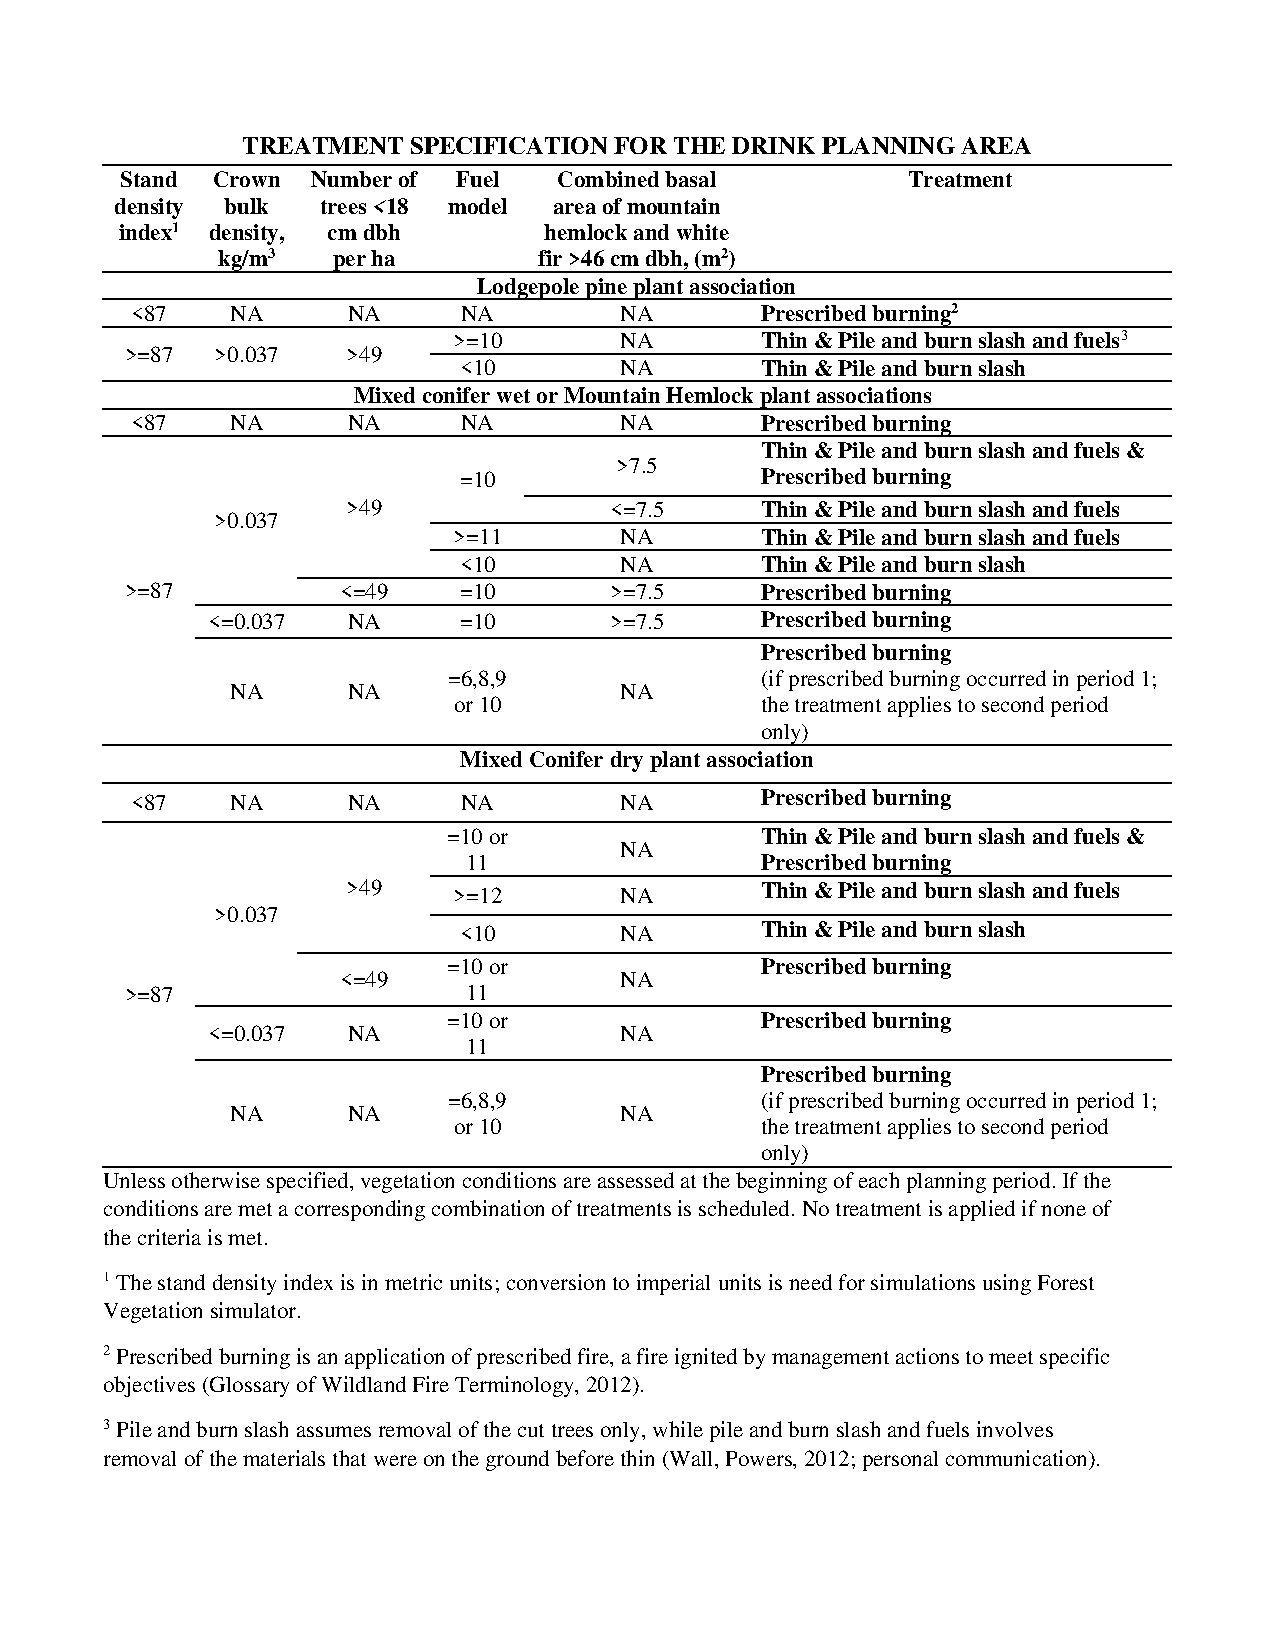
\includegraphics[width=\textwidth]{./appB/TreatmentSpecsForDrink.pdf}
%\end{figure}
%=-,scale=0.5,pagecommand=\subsection{blub}]{./appB/TreatmentSpecsForDrink.pdf}

Table \ref{tab:drinkTreatmentRules} provides a mapping from a treatment unit's vegetation conditions to the type of fuels removal to apply to the treatment unit. If a treatment unit's conditions do not correspond to any row in the table, then no action is taken. The table was adapted from Schroder \cite{schroder2016multi}. The plant association groups in the Drink area are shown in Figure \ref{fig:drinkPAGs}.

\begin{longtable}{p{.1\linewidth}p{.1\linewidth}p{.15\linewidth}p{.15\linewidth}p{.2\linewidth}p{.25\linewidth}}
\caption[Rules governing treatment assignments in the Drink.]{Rules governing treatment assignments.} \\
\label{tab:drinkTreatmentRules}\\
\hline
\textbf{SDI}\footnote{Stand Density Index, calculated in metric units (trees per ha).}    & \textbf{CBD}\footnote{Crown bulk density ($kg/m^3$)}   & \textbf{$\text{TPH}_{<18}$}\footnote{Number of trees per hectare whose diameter at breast height (DBH) is less than 18 cm}       & \textbf{Fuel model}\footnote{According to the Anderson rating system\cite{anderson1982aids}}  & $\text{\textbf{BA}}_{\text{MHD+WF,}>46}$\footnote{Basal area in $m^2$ of all mountain hemlock (MHD) and white fir (WF) trees with DBH $> 46 cm$.} & \textbf{Treatment}                                                                \\ \hline
\multicolumn{6}{c}{\textbf{Lodgepole pine (LPD) plant association}}                                                                                                                                                                                                                                                                                                   \\ \hline
$<87$                      & N/A                                                    & N/A                                                 & N/A                  & N/A                                                                                                     & \textbf{Prescribed burn}                                                        \\ \hline
\multirow{2}{*}{$\ge 87$}  & \multirow{2}{*}{$>0.037$}                     & \multirow{2}{*}{$> 49$}                    & $ \ge 10$       & N/A                                                                                                     & \textbf{Thin, pileburn slash and fuels}\footnote{Pileburning slash involves removal of thinned trees only, while pileburning slash and fuels also involves removal of materials that were on the ground before thinning (Wall, Powers, 2012; personal communication)}                                         \\ \cline{4-6} 
                                  &                                                        &                                                     &$< 10$         & N/A                                                                                                     & \textbf{Thin, pileburn slash}                                                     \\ \hline
\multicolumn{6}{c}{\textbf{Mixed conifer wet (MCW) or mountain hemlock (MHD) plant associations}}                                                                                                                                                                                                                                                                     \\ \hline
$<87$                       & N/A                                                    & N/A                                                 & N/A                  & N/A                                                                                                     & \textbf{Prescribed burn}                                                          \\ \hline
\multirow{7}{*}{$\ge 87$}  & \multirow{5}{*}{$>0.037$}                     & \multirow{4}{*}{$>49$}                     & \multirow{2}{*}{$=10$} & $>7.5$                                                                                         & \textbf{Thin, pileburn slash and fuels, prescribed burn}                          \\ \cline{5-6} 
                                  &                                                        &                                                     &                      & $ \le 7.5$                                                                                          & \textbf{Thin, pileburn slash and fuels}                                           \\ \cline{4-6} 
                                  &                                                        &                                                     & $>10$       & N/A                                                                                                     & \textbf{Thin, pileburn slash and fuels}                                           \\ \cline{4-6} 
                                  &                                                        &                                                     & $< 10$         & N/A                                                                                                     & \textbf{Thin, pileburn slash}                                                     \\ \cline{3-6} 
                                  &                                                        & $ \le 49$                                       & $=10$                  & $ \ge 7.5$                                                                                       & \textbf{Prescribed burn}                                                          \\ \cline{2-6} 
                                  & $ \le 0.037$                                        & N/A                                                 & $=10$                  & $\ge 7.5$                                                                                        & \textbf{Prescribed burn}                                                          \\ \cline{2-6} 
                                  & N/A                                                    & N/A                                                 & $\in \{6,8,9,10\}$            & N/A                                                                                                     & \textbf{Prescribed burn}\footnote{\label{footnote:p2TrtNote}Only if prescribed burn was assigned in period 1 (applies to period 2 treatment assignments only)} \\ \hline
\multicolumn{6}{c}{\textbf{Mixed conifer dry (MCD) plant association}}                                                                                                                                                                                                                                                                                                \\ \hline
$<87$                       & N/A                                                    & N/A                                                 & N/A                  & N/A                                                                                                     & \textbf{Prescribed burn}                                                          \\ \hline
\multirow{6}{*}{$ \ge 87$} & \multicolumn{1}{c}{\multirow{4}{*}{$ > 0.037$}} & \multicolumn{1}{c}{\multirow{3}{*}{$ >49$}} & $\in \{10,11\}$               & N/A                                                                                                     & \textbf{Thin, pileburn slash and fuels, prescribed burn}                          \\ \cline{4-6} 
                                  & \multicolumn{1}{c}{}                                   & \multicolumn{1}{c}{}                                & $\ge 12$      & N/A                                                                                                     & \textbf{Thin, pileburn slash and fuels}                                           \\ \cline{4-6} 
                                  & \multicolumn{1}{c}{}                                   & \multicolumn{1}{c}{}                                & $ < 10$          & N/A                                                                                                     & \textbf{Thin, pileburn slash}                                                     \\ \cline{3-6} 
                                  & \multicolumn{1}{c}{}                                   & $ \le 49$                                        & $\in \{10,11\}$               & N/A                                                                                                     & \textbf{Prescribed burn}                                                          \\ \cline{2-6} 
                                  & $\le 0.037$                                        & N/A                                                 & $\in \{10,11\}$               & N/A                                                                                                     & \textbf{Prescribed burn}                                                          \\ \cline{2-6} 
                                  & N/A                                                    & N/A                                                 & $\in \{6,8,9,10\}$            & N/A                                                                                                     & \textbf{Prescribed burn}\footnotemark[\ref{footnote:p2TrtNote}] \\
%\end{tabular}
\end{longtable}
%\end{table}

\begin{figure}
\centering
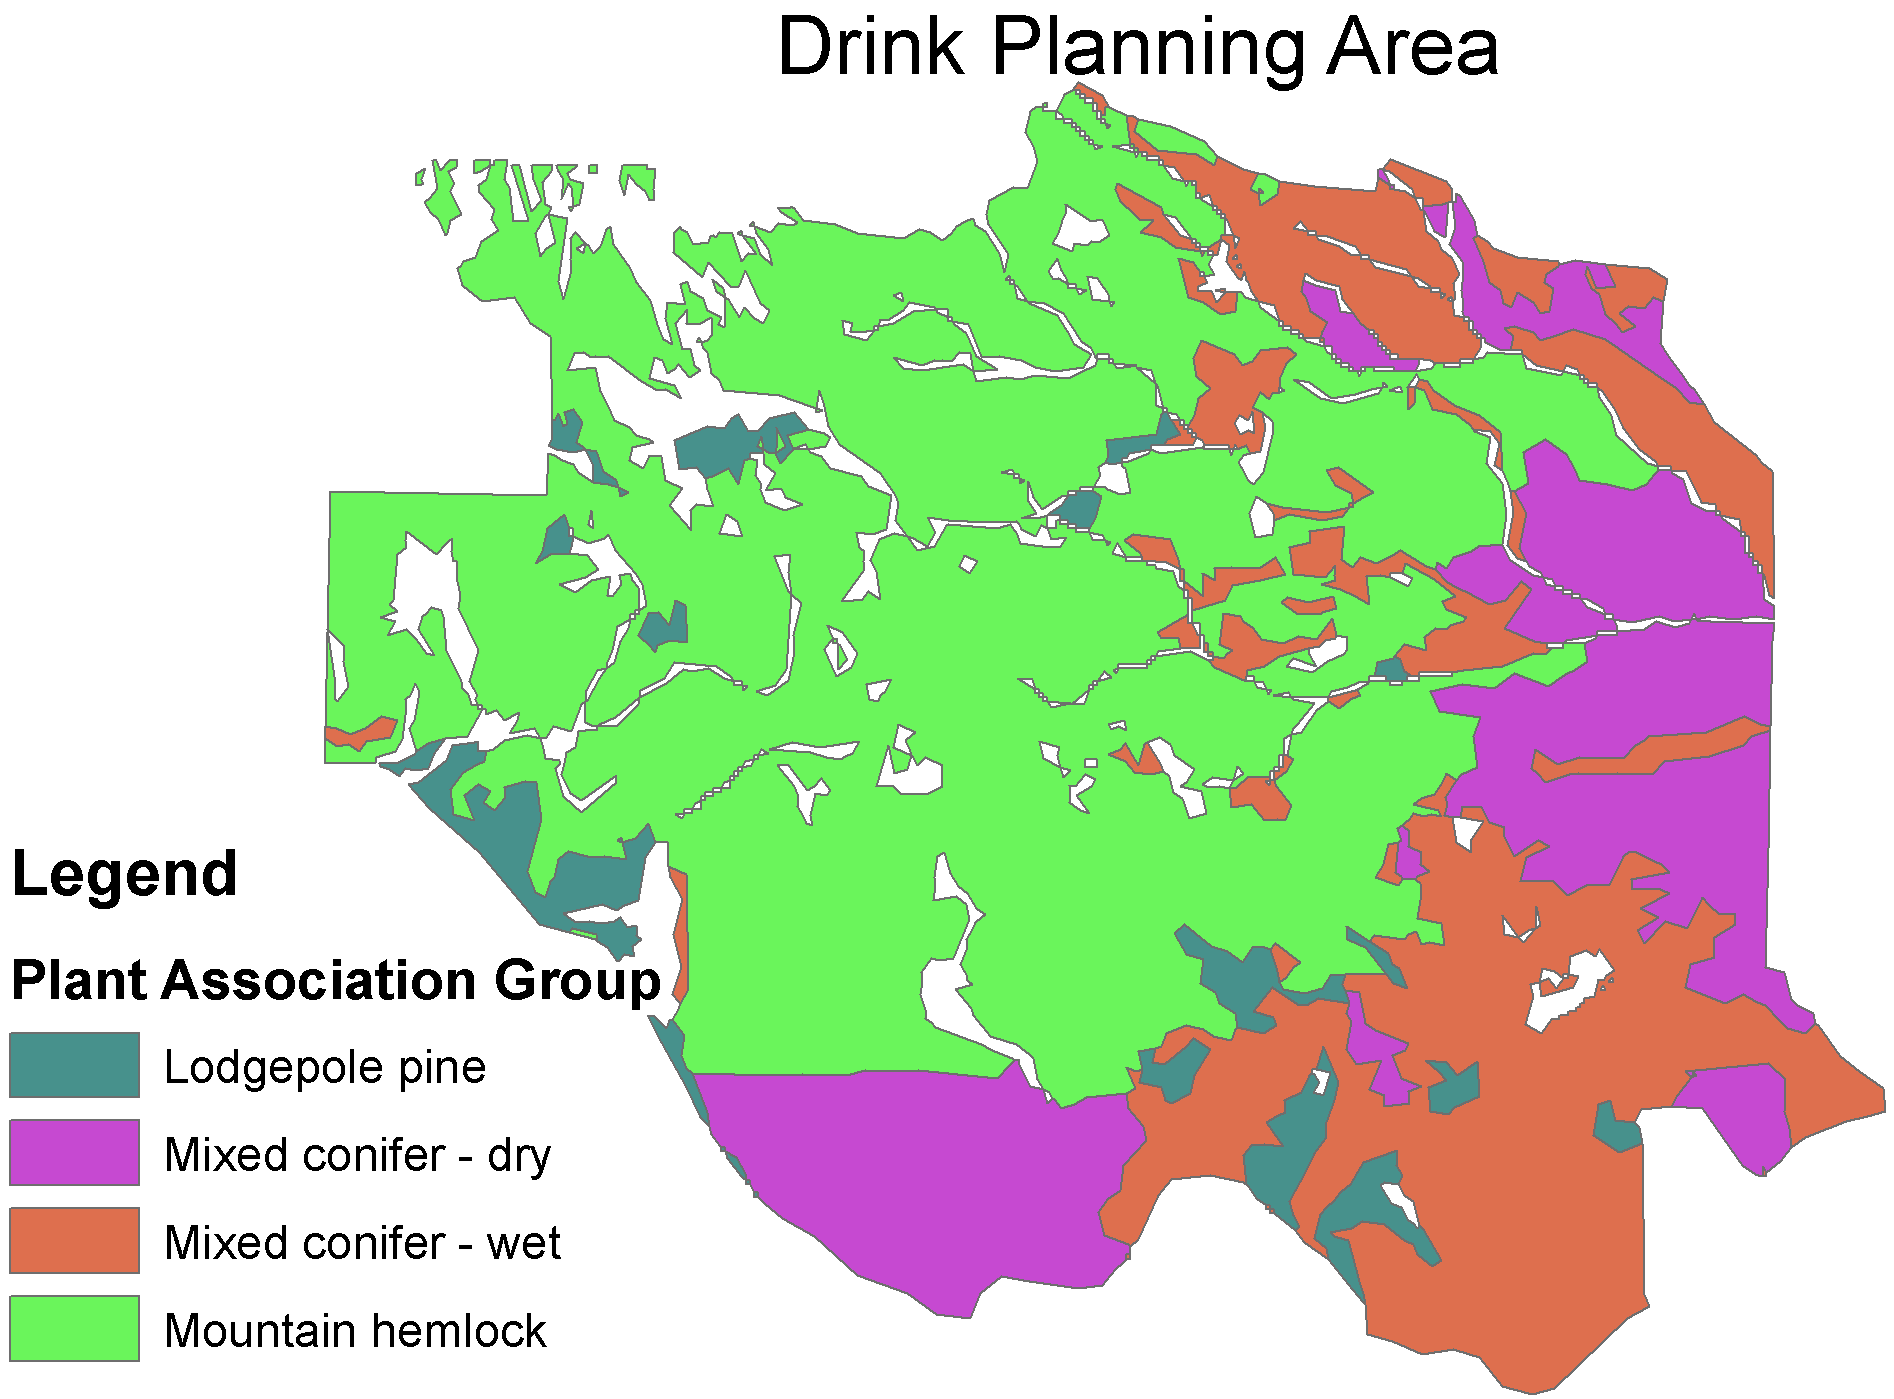
\includegraphics[width=.5\textwidth]{../images/DrinkMap_PAGs}
\caption[Plant association groups in the Drink Planning Area]{Plant association groups in the Drink Area that are considered for treatments.}
\label{fig:drinkPAGs}
\end{figure}


\end{document}